\documentclass{article}
\usepackage{filecontents}
\usepackage{tabularx}
\usepackage{longtable}
\usepackage{ltxtable}
\usepackage[latin1]{inputenc}
\usepackage{amssymb}
\usepackage{graphicx}
\usepackage{bmpsize}
\usepackage[T1]{fontenc}
\usepackage{parskip}
\usepackage{amsmath}
\usepackage[official]{eurosym}
\usepackage{mathrsfs}
\usepackage[justification=centering]{subfig}
\usepackage{hyperref}
\usepackage[english]{babel}
\usepackage{natbib}

\begin{filecontents}{job.bib}
@article{ashraf2008does,
  title={When does improving health raise GDP?},
  author={Ashraf, Quamrul H and Lester, Ashley and Weil, David N},
  journal={NBER macroeconomics annual},
  volume={23},
  number={1},
  pages={157--204},
  year={2008},
  publisher={The University of Chicago Press}
}
@article{who2016ebola,
  title={Ebola virus disease among male and female persons in West Africa},
  author={WHO Ebola Response Team},
  journal={New England Journal of Medicine},
  volume={374},
  number={1},
  pages={96--98},
  year={2016},
  publisher={Mass Medical Soc}
}
@article{who2015ebola,
  title={Ebola virus disease among children in West Africa},
  author={WHO Ebola Response Team},
  journal={New England Journal of Medicine},
  volume={372},
  number={13},
  pages={1274--1277},
  year={2015},
  publisher={Mass Medical Soc}
}
@article{fast2015role,
  title={The role of social mobilization in controlling Ebola virus in Lofa County, Liberia},
  author={Fast, Shannon M and Mekaru, Sumiko and Brownstein, John S and Postlethwaite, Timothy A and Markuzon, Natasha},
  journal={PLoS currents},
  volume={7},
  year={2015},
  publisher={Public Library of Science}
}
@article{ord2018retrospective,
  title={A Retrospective Analysis of the Spatial and Temporal Patterns of the West African Ebola Epidemic, 2014-2015},
  author={Ord, Keith and Getis, Arthur},
  journal={Geographical Analysis},
  volume={50},
  number={4},
  pages={337--357},
  year={2018},
  publisher={Wiley Online Library}
}
@article{ravi2019review,
  title={Review of international efforts to strengthen the global outbreak response system since the 2014--16 West Africa Ebola Epidemic},
  author={Ravi, Sanjana J and Snyder, Michael R and Rivers, Caitlin},
  journal={Health policy and planning},
  volume={34},
  number={1},
  pages={47--54},
  year={2019},
  publisher={Oxford University Press}
}
@article{frontieres2015pushed,
  title={Pushed to the limit and beyond: a year into the largest ever Ebola outbreak.},
  author={Fronti{\`e}res, M{\'e}decins Sans},
  year={2015},
  publisher={Medecins Sans Frontieres}
}
@article{alexander2015factors,
  title={What factors might have led to the emergence of Ebola in West Africa?},
  author={Alexander, Kathleen A and Sanderson, Claire E and Marathe, Madav and Lewis, Bryan L and Rivers, Caitlin M and Shaman, Jeffrey and Drake, John M and Lofgren, Eric and Dato, Virginia M and Eisenberg, Marisa C and others},
  journal={PLoS neglected tropical diseases},
  volume={9},
  number={6},
  pages={e0003652},
  year={2015},
  publisher={Public Library of Science}
}
@article{van2015review,
  title={A review of epidemiological parameters from Ebola outbreaks to inform early public health decision-making},
  author={Van Kerkhove, Maria D and Bento, Ana I and Mills, Harriet L and Ferguson, Neil M and Donnelly, Christl A},
  journal={Scientific data},
  volume={2},
  pages={150019},
  year={2015},
  publisher={Nature Publishing Group}
}
@article{goeijenbier2014ebola,
  title={Ebola virus disease: a review on epidemiology, symptoms, treatment and pathogenesis},
  author={Goeijenbier, Marco and Van Kampen, JJ and Reusken, CB and Koopmans, MP and Van Gorp, EC and others},
  journal={Neth J Med},
  volume={72},
  number={9},
  pages={442--8},
  year={2014}
}
@article{thomas2015economic,
  title={The economic impact of ebola on sub Saharan Africa: updated estimates for 2015},
  author={Thomas, Mark Roland and Smith, Gregory and Ferreira, Francisco HG and Evans, David and Maliszewska, Maryla and Cruz, Marcio and Himelein, Kristen and Over, Mead},
  year={2015}
}
@misc{stock2002testing,
  title={Testing for weak instruments in linear IV regression},
  author={Stock, James H and Yogo, Motohiro},
  year={2002},
  publisher={National Bureau of Economic Research Cambridge, Mass., USA}
}
@article{feenstra2018search,
  title={In search of the Armington elasticity},
  author={Feenstra, Robert C and Luck, Philip and Obstfeld, Maurice and Russ, Katheryn N},
  journal={Review of Economics and Statistics},
  volume={100},
  number={1},
  pages={135--150},
  year={2018},
  publisher={MIT Press}
}
@article{heathcote2002financial,
  title={Financial autarky and international business cycles},
  author={Heathcote, Jonathan and Perri, Fabrizio},
  journal={Journal of monetary Economics},
  volume={49},
  number={3},
  pages={601--627},
  year={2002},
  publisher={Elsevier}
}
@article{armington1969theory,
  title={A theory of demand for products distinguished by place of production},
  author={Armington, Paul S},
  journal={Staff Papers},
  volume={16},
  number={1},
  pages={159--178},
  year={1969},
  publisher={Springer}
}
@article{ravn2002adjusting,
  title={On adjusting the Hodrick-Prescott filter for the frequency of observations},
  author={Ravn, Morten O and Uhlig, Harald},
  journal={Review of economics and statistics},
  volume={84},
  number={2},
  pages={371--376},
  year={2002},
  publisher={MIT Press}
}
@article{fisman2014early,
  title={Early epidemic dynamics of the West African 2014 Ebola outbreak estimates derived with a simple two parameter model},
  author={Fisman, David and Khoo, Edwin and Tuite, Ashleigh},
  journal={PLoS currents},
  volume={6},
  year={2014},
  publisher={Public Library of Science}
}
@article{smets2007shocks,
  title={Shocks and frictions in US business cycles: A Bayesian DSGE approach},
  author={Smets, Frank and Wouters, Rafael},
  journal={American economic review},
  volume={97},
  number={3},
  pages={586--606},
  year={2007}
}
@article{schmitt2003closing,
  title={Closing small open economy models},
  author={Schmitt-Groh{\'e}, Stephanie and Uribe, Mart{\i}n},
  journal={Journal of international Economics},
  volume={61},
  number={1},
  pages={163--185},
  year={2003},
  publisher={Elsevier}
}
@article{kim2003spurious,
  title={Spurious welfare reversals in international business cycle models},
  author={Kim, Jinill and Kim, Sunghyun Henry},
  journal={journal of International Economics},
  volume={60},
  number={2},
  pages={471--500},
  year={2003},
  publisher={Elsevier}
}
@article{adjemian2011dynare,
  title={Dynare: Reference manual, version 4},
  author={Adjemian, St{\'e}phane and Bastani, Houtan and Juillard, Michel and Mihoubi, Ferhat and Perendia, George and Ratto, Marco and Villemot, S{\'e}bastien},
  year={2011},
  publisher={Dynare working papers 1, CEPREMAP}
}
@techreport{djogbenou2018asymptotic,
  title={Asymptotic theory and wild bootstrap inference with clustered errors},
  author={Djogbenou, Antoine A and MacKinnon, James G and Orregaard Nielsen, Morten},
  year={2018}
}
@article{mackinnon2018wild,
  title={The wild bootstrap for few (treated) clusters},
  author={MacKinnon, James G and Webb, Matthew D},
  journal={The Econometrics Journal},
  volume={21},
  number={2},
  pages={114--135},
  year={2018},
  publisher={Oxford University Press Oxford, UK}
}
@article{roodman2019fast,
  title={Fast and wild: Bootstrap inference in Stata using boottest},
  author={Roodman, David and Nielsen, Morten {\O}rregaard and MacKinnon, James G and Webb, Matthew D},
  journal={The Stata Journal},
  volume={19},
  number={1},
  pages={4--60},
  year={2019},
  publisher={SAGE Publications Sage CA: Los Angeles, CA}
}
@article{donald2007inference,
  title={Inference with difference-in-differences and other panel data},
  author={Donald, Stephen G and Lang, Kevin},
  journal={The review of Economics and Statistics},
  volume={89},
  number={2},
  pages={221--233},
  year={2007},
  publisher={MIT Press}
}
@article{cameron2008bootstrap,
  title={Bootstrap-based improvements for inference with clustered errors},
  author={Cameron, A Colin and Gelbach, Jonah B and Miller, Douglas L},
  journal={The Review of Economics and Statistics},
  volume={90},
  number={3},
  pages={414--427},
  year={2008},
  publisher={MIT Press}
}
@article{conley2011inference,
  title={Inference with difference in differences with a small number of policy changes},
  author={Conley, Timothy G and Taber, Christopher R},
  journal={The Review of Economics and Statistics},
  volume={93},
  number={1},
  pages={113--125},
  year={2011},
  publisher={MIT Press}
}
@article{mackinnon2017wild,
  title={Wild bootstrap inference for wildly different cluster sizes},
  author={MacKinnon, James G and Webb, Matthew D},
  journal={Journal of Applied Econometrics},
  volume={32},
  number={2},
  pages={233--254},
  year={2017},
  publisher={Wiley Online Library}
}
@article{carter2017asymptotic,
  title={Asymptotic behavior of at-test robust to cluster heterogeneity},
  author={Carter, Andrew V and Schnepel, Kevin T and Steigerwald, Douglas G},
  journal={Review of Economics and Statistics},
  volume={99},
  number={4},
  pages={698--709},
  year={2017},
  publisher={MIT Press}
}

@article{moulton1990illustration,
  title={An illustration of a pitfall in estimating the effects of aggregate variables on micro unit},
  author={Moulton, Brent R and others},
  journal={The review of Economics and Statistics},
  volume={72},
  number={2},
  pages={334--338},
  year={1990},
  publisher={MIT Press}
}
@article{ledgerwood2017chimpanzee,
  title={Chimpanzee adenovirus vector Ebola vaccine},
  author={Ledgerwood, Julie E and DeZure, Adam D and Stanley, Daphne A and Coates, Emily E and Novik, Laura and Enama, Mary E and Berkowitz, Nina M and Hu, Zonghui and Joshi, Gyan and Ploquin, Aur{\'e}lie and others},
  journal={New England Journal of Medicine},
  volume={376},
  number={10},
  pages={928--938},
  year={2017},
  publisher={Mass Medical Soc}
}
@article{baggi2014management,
  title={Management of pregnant women infected with Ebola virus in a treatment centre in Guinea, June 2014},
  author={Baggi, FM and Taybi, A and Kurth, Andreas and Van Herp, M and Di Caro, A and Wolfel, R and Gunther, S and Decroo, T and Declerck, H and Jonckheere, S},
  journal={Eurosurveillance},
  year={2014},
  publisher={European Centre for Disease Prevention and Control}
}
@article{dornemann2017first,
  title={First newborn baby to receive experimental therapies survives Ebola virus disease},
  author={D{\"o}rnemann, Jenny and Burzio, Chiara and Ronsse, Axelle and Sprecher, Armand and De Clerck, Hilde and Van Herp, Michel and Koli{\'e}, Marie-Claire and Yosifiva, Vesselina and Caluwaerts, Severine and McElroy, Anita K and others},
  journal={The Journal of infectious diseases},
  volume={215},
  number={2},
  pages={171--174},
  year={2017},
  publisher={Oxford University Press}
}
@book{bhattacharya2013health,
  title={Health economics},
  author={Bhattacharya, Jay and Hyde, Timothy and Tu, Peter},
  year={2013},
  publisher={Macmillan International Higher Education}
}
@article{hansen2017preventing,
  title={Preventing the White Death: Tuberculosis Dispensaries},
  author={Hansen, Casper Worm and Jensen, Peter S and Egedes{\o}, Peter},
  journal={Available at SSRN 3036887},
  year={2017}
}
@article{bjornstad2002dynamics,
  title={Dynamics of measles epidemics, estimating scaling of transmission rates using a time series SIR model},
  author={Bj{\o}rnstad, Ottar N and Finkenst{\"a}dt, B{\"a}rbel F and Grenfell, Bryan T},
  journal={Ecological monographs},
  volume={72},
  number={2},
  pages={169--184},
  year={2002},
  publisher={Wiley Online Library}
}
@article{mccluskey2010complete,
  title={Complete global stability for an SIR epidemic model with delay distributed or discrete},
  author={McCluskey, C Connell},
  journal={Nonlinear Analysis, Real World Applications},
  volume={11},
  number={1},
  pages={55--59},
  year={2010},
  publisher={Elsevier}
}
@article{shulgin1998pulse,
  title={Pulse vaccination strategy in the SIR epidemic model},
  author={Shulgin, Boris and Stone, Lewi and Agur, Zvia},
  journal={Bulletin of mathematical biology},
  volume={60},
  number={6},
  pages={1123--1148},
  year={1998},
  publisher={Springer}
}
@article{kermack1927contribution,
  title={A contribution to the mathematical theory of epidemics},
  author={Kermack, William O and McKendrick, Anderson G},
  journal={Proceedings of the royal society of london. Series A, Containing papers of a mathematical and physical character},
  volume={115},
  number={772},
  pages={700--721},
  year={1927},
  publisher={JSTOR}
}
@article{jayachandran2009life,
  title={Life expectancy and human capital investments: Evidence from maternal mortality declines},
  author={Jayachandran, Seema and Lleras-Muney, Adriana},
  journal={The Quarterly Journal of Economics},
  volume={124},
  number={1},
  pages={349--397},
  year={2009},
  publisher={MIT Press}
}
@book{evans2015next,
  title={The next wave of deaths from Ebola? the impact of health care worker mortality},
  author={Evans, David K and Goldstein, Markus and Popova, Anna},
  year={2015},
  publisher={The World Bank}
}
@article{becerra2014foreign,
  title={Foreign aid in the aftermath of large natural disasters},
  author={Becerra, Oscar and Cavallo, Eduardo and Noy, Ilan},
  journal={Review of Development Economics},
  volume={18},
  number={3},
  pages={445--460},
  year={2014},
  publisher={Wiley Online Library}
}
@article{rowe1999clinical,
  title={Clinical, virologic, and immunologic follow-up of convalescent Ebola hemorrhagic fever patients and their household contacts, Kikwit, Democratic Republic of the Congo},
  author={Rowe, Alexander K and Bertolli, Jeanne and Khan, Ali S and Mukunu, Rose and Muyembe-Tamfum, JJ and Bressler, David and Williams, AJ and Peters, CJ and Rodriguez, Luis and Feldmann, Heinz and others},
  journal={The Journal of infectious diseases},
  volume={179},
  number={Supplement\_1},
  pages={S28--S35},
  year={1999},
  publisher={The University of Chicago Press}
}
@article{clark2015long,
  title={Long-term sequelae after Ebola virus disease in Bundibugyo, Uganda - a retrospective cohort study},
  author={Clark, Danielle V and Kibuuka, Hannah and Millard, Monica and Wakabi, Salim and Lukwago, Luswa and Taylor, Alison and Eller, Michael A and Eller, Leigh Anne and Michael, Nelson L and Honko, Anna N and others},
  journal={The Lancet Infectious Diseases},
  volume={15},
  number={8},
  pages={905--912},
  year={2015},
  publisher={Elsevier}
}
@article{world2016latest,
  title={Latest Ebola outbreak over in Liberia, West Africa is at zero, but new flare-ups are likely to occur},
  author={World Health Organization and others},
  journal={Retrieved January},
  volume={14},
  pages={2016},
  year={2016}
}
@misc{blanchard1988dynamic,
  title={The dynamic effects of aggregate demand and supply disturbances},
  author={Blanchard, Olivier J and Quah, Danny},
  year={1988},
  publisher={National Bureau of Economic Research Cambridge, Mass., USA}
}
@techreport{freyal2018pre,
  title={Pre event trends in the panel event study design},
  author={Freyaldenhoven, Simon and Hansen, Christian and Shapiro, Jesse M},
  year={2018},
  institution={National Bureau of Economic Research}
}
@article{borusyak2017revisiting,
  title={Revisiting event study designs},
  author={Borusyak, Kirill and Jaravel, Xavier},
  journal={Available at SSRN 2826228},
  year={2017}
}

@article{ehrhardt2006malaria,
  title={Malaria, anemia, and malnutrition in African children defining intervention priorities},
  author={Ehrhardt, Stephan and Burchard, Gerd D and Mantel, Carsten and Cramer, Jakob P and Kaiser, Sarah and Kubo, Martina and Otchwemah, Rowland N and Bienzle, Ulrich and Mockenhaupt, Frank P},
  journal={The Journal of infectious diseases},
  volume={194},
  number={1},
  pages={108--114},
  year={2006},
  publisher={The University of Chicago Press}
}
@article{who2014ebola,
  title={Ebola virus disease in West Africa, the first 9 months of the epidemic and forward projections},
  author={WHO Ebola Response Team},
  journal={New England Journal of Medicine},
  volume={371},
  number={16},
  pages={1481--1495},
  year={2014},
  publisher={Mass Medical Soc}
}
@article{parpia2016effects,
  title={Effects of response to 2014--2015 Ebola outbreak on deaths from malaria, HIV/AIDS, and tuberculosis, West Africa},
  author={Parpia, Alyssa S and Ndeffo-Mbah, Martial L and Wenzel, Natasha S and Galvani, Alison P},
  journal={Emerging infectious diseases},
  volume={22},
  number={3},
  pages={433},
  year={2016},
  publisher={Centers for Disease Control and Prevention}
}
@article{meghir2018education,
  title={Education and mortality: Evidence from a social experiment},
  author={Meghir, Costas and Palme, M{\aa}rten and Simeonova, Emilia},
  journal={American Economic Journal: Applied Economics},
  volume={10},
  number={2},
  pages={234--56},
  year={2018}
}
@article{clark2013effect,
  title={The effect of education on adult mortality and health: Evidence from Britain},
  author={Clark, Damon and Royer, Heather},
  journal={American Economic Review},
  volume={103},
  number={6},
  pages={2087--2120},
  year={2013}
}
@article{preston1975changing,
  title={The changing relation between mortality and level of economic development},
  author={Preston, Samuel H},
  journal={Population studies},
  volume={29},
  number={2},
  pages={231--248},
  year={1975},
  publisher={Taylor \& Francis}
}
@article{cohen2004social,
  title={Social relationships and health.},
  author={Cohen, Sheldon},
  journal={American psychologist},
  volume={59},
  number={8},
  pages={676},
  year={2004},
  publisher={American Psychological Association}
}
@article{thoits2010stress,
  title={Stress and health: Major findings and policy implications},
  author={Thoits, Peggy A},
  journal={Journal of health and social behavior},
  volume={51},
  number={1\_suppl},
  pages={S41--S53},
  year={2010},
  publisher={Sage Publications Sage CA: Los Angeles, CA}
}
@article{arcaya2015inequalities,
  title={Inequalities in health: definitions, concepts, and theories},
  author={Arcaya, Mariana C and Arcaya, Alyssa L and Subramanian, SV},
  journal={Global health action},
  volume={8},
  number={1},
  pages={27106},
  year={2015},
  publisher={Taylor \& Francis}
}
@article{lozano2012global,
  title={Global and regional mortality from 235 causes of death for 20 age groups in 1990 and 2010: a systematic analysis for the Global Burden of Disease Study 2010},
  author={Lozano, Rafael and Naghavi, Mohsen and Foreman, Kyle and Lim, Stephen and Shibuya, Kenji and Aboyans, Victor and Abraham, Jerry and Adair, Timothy and Aggarwal, Rakesh and Ahn, Stephanie Y and others},
  journal={The lancet},
  volume={380},
  number={9859},
  pages={2095--2128},
  year={2012},
  publisher={Elsevier}
}
@article{soares2007determinants,
  title={On the determinants of mortality reductions in the developing world},
  author={Soares, Rodrigo R},
  journal={Population and Development Review},
  volume={33},
  number={2},
  pages={247--287},
  year={2007},
  publisher={Wiley Online Library}
}
@article{marmot2005social,
  title={Social determinants of health inequalities},
  author={Marmot, Michael},
  journal={The lancet},
  volume={365},
  number={9464},
  pages={1099--1104},
  year={2005},
  publisher={Elsevier}
}
@article{cook2008internet,
  title={Internet-based learning in the health professions: a meta-analysis},
  author={Cook, David A and Levinson, Anthony J and Garside, Sarah and Dupras, Denise M and Erwin, Patricia J and Montori, Victor M},
  journal={Jama},
  volume={300},
  number={10},
  pages={1181--1196},
  year={2008},
  publisher={American Medical Association}
}
@article{cutler2006determinants,
  title={The determinants of mortality},
  author={Cutler, David and Deaton, Angus and Lleras-Muney, Adriana},
  journal={Journal of economic perspectives},
  volume={20},
  number={3},
  pages={97--120},
  year={2006}
}
@article{kieh2009roots,
  title={The roots of the second Liberian civil war},
  author={Kieh Jr, George Klay},
  journal={International Journal on World Peace},
  pages={7--30},
  year={2009},
  publisher={JSTOR}
}
@article{neiderud2015urbanization,
  title={How urbanization affects the epidemiology of emerging infectious diseases},
  author={Neiderud, Carl-Johan},
  journal={Infection ecology \& epidemiology},
  volume={5},
  number={1},
  pages={27060},
  year={2015},
  publisher={Taylor \& Francis}
}
@article{dalziel2018urbanization,
  title={Urbanization and humidity shape the intensity of influenza epidemics in US cities},
  author={Dalziel, Benjamin D and Kissler, Stephen and Gog, Julia R and Viboud, Cecile and Bj{\o}rnstad, Ottar N and Metcalf, C Jessica E and Grenfell, Bryan T},
  journal={Science},
  volume={362},
  number={6410},
  pages={75--79},
  year={2018},
  publisher={American Association for the Advancement of Science}
}
@article{bertrand2004much,
  title={How much should we trust differences-in-differences estimates?},
  author={Bertrand, Marianne and Duflo, Esther and Mullainathan, Sendhil},
  journal={The Quarterly journal of economics},
  volume={119},
  number={1},
  pages={249--275},
  year={2004},
  publisher={MIT Press}
}
@article{autor2003outsourcing,
  title={Outsourcing at will: The contribution of unjust dismissal doctrine to the growth of employment outsourcing},
  author={Autor, David H},
  journal={Journal of labor economics},
  volume={21},
  number={1},
  pages={1--42},
  year={2003},
  publisher={The University of Chicago Press}
}
@article{pischke2005empirical,
  title={Empirical Methods in Applied Economics: Lecture Notes},
  author={Pischke, Jorn-Steffen},
  journal={Downloaded April},
  volume={24},
  pages={2019},
  year={2005}
}
@article{yearbook2007united,
  title={United Nations},
  author={Yearbook, Demographic},
  journal={New York},
  number={38},
  year={2007}
}
@article{de1996recensement,
  title={Recensement G{\'e}n{\'e}ral de la Population},
  author={de la Statistique, Direction},
  journal={R{\'e}publique de Guin{\'e}e. Conakry: minist{\`e}re du Plan},
  year={1996}
}
@article{leone2015population,
  title={Population and Housing Census: Summary of Final Results. Planning a Better Future},
  author={Leone, Statistics Sierra},
  journal={Freetown: Author},
  year={2015}
}
@techreport{freyaldenhoven2018pre,
  title={Pre-event trends in the panel event-study design},
  author={Freyaldenhoven, Simon and Hansen, Christian and Shapiro, Jesse M},
  year={2018},
  institution={National Bureau of Economic Research}
}
@article{chan2011using,
  title={Using web search query data to monitor dengue epidemics: a new model for neglected tropical disease surveillance},
  author={Chan, Emily H and Sahai, Vikram and Conrad, Corrie and Brownstein, John S},
  journal={PLoS neglected tropical diseases},
  volume={5},
  number={5},
  pages={e1206},
  year={2011},
  publisher={Public Library of Science}
}
@article{ginsberg2009detecting,
  title={Detecting influenza epidemics using search engine query data},
  author={Ginsberg, Jeremy and Mohebbi, Matthew H and Patel, Rajan S and Brammer, Lynnette and Smolinski, Mark S and Brilliant, Larry},
  journal={Nature},
  volume={457},
  number={7232},
  pages={1012},
  year={2009},
  publisher={Nature Publishing Group}
}
@article{althaus2014estimating,
  title={Estimating the reproduction number of Ebola virus (EBOV) during the 2014 outbreak in West Africa},
  author={Althaus, Christian L},
  journal={PLoS currents},
  volume={6},
  year={2014},
  publisher={Public Library of Science}
}
@article{norman2012long,
  title={The long-term health consequences of child physical abuse, emotional abuse, and neglect: a systematic review and meta-analysis},
  author={Norman, Rosana E and Byambaa, Munkhtsetseg and De, Rumna and Butchart, Alexander and Scott, James and Vos, Theo},
  journal={PLoS medicine},
  volume={9},
  number={11},
  pages={e1001349},
  year={2012},
  publisher={Public Library of Science}
}
@article{almond2011killing,
  title={Killing me softly: The fetal origins hypothesis},
  author={Almond, Douglas and Currie, Janet},
  journal={Journal of economic perspectives},
  volume={25},
  number={3},
  pages={153--72},
  year={2011}
}
@article{adda2016economic,
  title={Economic activity and the spread of viral diseases: Evidence from high frequency data},
  author={Adda, J{\'e}r{\^o}me},
  journal={The Quarterly Journal of Economics},
  volume={131},
  number={2},
  pages={891--941},
  year={2016},
  publisher={MIT Press}
}
@article{alsan2015effect,
  title={The effect of the tsetse fly on African development},
  author={Alsan, Marcella},
  journal={American Economic Review},
  volume={105},
  number={1},
  pages={382--410},
  year={2015}
}
@techreport{gonzalez2017epidemics,
  title={Epidemics and Conflict- Evidence from the Ebola outbreak in Western Africa},
  author={Gonzalez-Torres, Ada and Esposito, Elena},
  year={2017},
  institution={Working Paper}
}
@article{galiani2017synth_runner,
  title={The synth\_runner package- Utilities to automate synthetic control estimation using synth},
  author={Galiani, Sebastian and Quistorff, Brian},
  journal={The Stata Journal},
  volume={17},
  number={4},
  pages={834--849},
  year={2017},
  publisher={SAGE Publications Sage CA, Los Angeles, CA}
}
@article{abadie2010synthetic,
  title={Synthetic control methods for comparative case studies - Estimating the effect of California’s tobacco control program},
  author={Abadie, Alberto and Diamond, Alexis and Hainmueller, Jens},
  journal={Journal of the American statistical Association},
  volume={105},
  number={490},
  pages={493--505},
  year={2010},
  publisher={Taylor \& Francis}
}
@article{athey2017state,
  title={The state of applied econometrics- Causality and policy evaluation},
  author={Athey, Susan and Imbens, Guido W},
  journal={Journal of Economic Perspectives},
  volume={31},
  number={2},
  pages={3--32},
  year={2017}
}
@techreport{doudchenko2016balancing,
  title={Balancing, regression, difference-in-differences and synthetic control methods: A synthesis},
  author={Doudchenko, Nikolay and Imbens, Guido W},
  year={2016},
  institution={National Bureau of Economic Research}
}
@article{ferman2017cherry,
  title={Cherry picking with synthetic controls},
  author={Ferman, Bruno and Pinto, Cristine and Possebom, Vitor},
  year={2017}
}
@article{jorda2005estimation,
  title={Estimation and inference of impulse responses by local projections},
  author={Jord{\`a}, {\`O}scar},
  journal={American economic review},
  volume={95},
  number={1},
  pages={161--182},
  year={2005}
}
@article{bloom2014disease,
  title={Disease and development revisited},
  author={Bloom, David E and Canning, David and Fink, G{\"u}nther},
  journal={Journal of Political Economy},
  volume={122},
  number={6},
  pages={1355--1366},
  year={2014},
  publisher={University of Chicago Press Chicago, IL}
}
@article{stiglitz2009trade,
  title={Trade agreements and health in developing countries},
  author={Stiglitz, Joseph E},
  journal={The Lancet},
  volume={373},
  number={9661},
  pages={363--365},
  year={2009},
  publisher={Elsevier}
}
@article{smith2009trade,
  title={Trade in health-related services},
  author={Smith, Richard D and Chanda, Rupa and Tangcharoensathien, Viroj},
  journal={The Lancet},
  volume={373},
  number={9663},
  pages={593--601},
  year={2009},
  publisher={Elsevier}
}
@article{lopez2017trade,
  title={Is trade liberalisation a vector for the spread of sugar-sweetened beverages?},
  author={Lopez, Ana Mendez and Loopstra, Rachel and McKee, Martin and Stuckler, David},
  journal={Social Science \& Medicine},
  volume={172},
  pages={21--27},
  year={2017},
  publisher={Elsevier}
}
@article{weil2014health,
  title={Health and economic growth},
  author={Weil, David N},
  journal={Handbook of economic growth},
  volume={2},
  pages={623--682},
  year={2014},
  publisher={Elsevier}
}
@article{bloom2018health,
  title={Health and economic growth},
  author={Bloom, David E and Kuhn, Michael and Prettner, Klaus},
  year = {2018},
  journal={IZA Discussion Paper}
}
@article{acemoglu2007disease,
  title={Disease and development: the effect of life expectancy on economic growth},
  author={Acemoglu, Daron and Johnson, Simon},
  journal={Journal of political Economy},
  volume={115},
  number={6},
  pages={925--985},
  year={2007},
  publisher={The University of Chicago Press}
}
@article{mcmichael2004mortality,
  title={Mortality trends and setbacks: global convergence or divergence?},
  author={McMichael, Anthony J and McKee, Martin and Shkolnikov, Vladimir and Valkonen, Tapani},
  journal={The Lancet},
  volume={363},
  number={9415},
  pages={1155--1159},
  year={2004},
  publisher={Elsevier}
}
@article{chowell2014transmission,
  title={Transmission dynamics and control of Ebola virus disease (EVD): a review},
  author={Chowell, Gerardo and Nishiura, Hiroshi},
  journal={BMC medicine},
  volume={12},
  number={1},
  pages={196},
  year={2014},
  publisher={BioMed Central}
}
@article{ebola2015nyt, 
  title={Yes, We Were Warned About Ebola}, 
  url={https://www.nytimes.com/2015/04/08/opinion/yes-we-were-warned-about-ebola.html}, 
  journal={The New York Times}, 
  author={Nutt, Cameron and Mussah, Vera and Dahn, Bernice}, 
  year={2015}, 
  month={Apr}, 
}
@article{backus1992international,
  title={International real business cycles},
  author={Backus, David K and Kehoe, Patrick J and Kydland, Finn E},
  journal={Journal of political Economy},
  volume={100},
  number={4},
  pages={745--775},
  year={1992},
  publisher={The University of Chicago Press}
}
@misc{wdi,
title = {World Development Indicators},
author = {{The World Bank}},
url = {http://datatopics.worldbank.org/world-development-indicators/},
year = {2017}
}
@misc{whostatistics,
title = {Global Health Workforce Statistics},
author = {{World Health Organization}},
url = {http://www.who.int/hrh/statistics/hwfstats/},
year = {2018}
}
@misc{imfdot,
title = {Directions of Trade},
author = {{International Monetary Fund}},
year = {2017},
institution = {International Monetary Fund},
type = {Time series data},
url = {http://data.imf.org/?sk=9D6028D4-F14A-464C-A2F2-59B2CD424B85}
}
@misc{whoebola,
title = {Ebola Situation Reports: Archive},
author = {{World Health Organisation}},
year = {2016},
month = {June},
institution = {World Health Organisation},
type = {Time series data},
url = {https://www.who.int/csr/disease/ebola/situation-reports/archive/en/}
}
\end{filecontents}

\begin{document}

\begin{titlepage}
\pagestyle{empty}
\Large
\begin{center}
\vspace*{2.5 cm} \LARGE
\textbf{Health And Trade - Investigating The 2014 Ebola Outbreak}\\
\Large \vspace*{2.5 cm}
Marius Gruenewald\\\vspace{0.375 cm}
marius{\_}gruenewald@web.de \\\vspace{0.375 cm}
01.05.2019 \\ \vspace{0.375 cm}
Department of Economics, UW - Madison \\ 
\textbf{}\\
\textbf{Abstract}\\
{\normalsize Over the last years, research on the impact of globalization on health has sky-rocketed. Despite, there has been, to the best of my knowledge, no research that investigates the reverse causality. This gap gives the main motivation for my research design. I offer a first step for a theoretical consideration of health determined trade. Later, the suggested identification strategy for empirical estimation is a natural experiment. I argue that the 2014 Ebola outbreak in western Africa can be treated as such by providing mostly anecdotal evidence. Lastly, a discussion of data will be provided.}
\end{center}
\vspace{2.5 cm}
\end{titlepage}

\pagebreak
\pagestyle{plain}
\pagenumbering{Roman}
\newpage
\setcounter{page}{2}
\pagenumbering{arabic}
\setlength{\baselineskip}{1\baselineskip}
\pagestyle{plain}

\section{Motivation}

Over the course of the last years there has been a surge of scholastic studies dealing with the consequences of globalization on health outcomes (the Lancet series on trade and health). This is not surprising given the interesting data connection we observe when comparing the time trends as shown in figure \ref{Exports and Health}.

\begin{figure}[!ht]
\begin{center}\caption{Exports and Health \label{Exports and Health}}
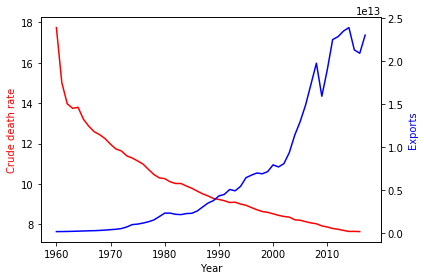
\includegraphics[width=0.7\textwidth]{C:/Users/mariu/Documents/Master_Thesis/Master_thesis/Pics_graphs/Trade_Health_World.png}\\
\end{center}
\end{figure}

There is an obvious correlation in the data. Correlations usually leave us with the question of whether a causal mechanism is in play, and if, in which direction, or it follows a third common factor.\\
A brief literature review lays out an expansive body of literature investigating the effect of trade on health. Most notably, a Lancet series including contributions by \cite{stiglitz2009trade} and \cite{smith2009trade} and outside the series \cite{lopez2017trade}. Yet, valuable insight can be gained by considering the literature investigating the relationship of health on growth, since approaches and methods are closely aligned. \cite{weil2014health} offers an excellent literature review of the related topic. More recently, \cite{bloom2018health} discuss the topic with respect to empirical difficulties and contextual issues.

\section{Trade and Health}

\section{Ebola Virus Disease}
The Ebola Virus Disease (EVD) is a rare, infectious disease of the taxonomic family \textit{Filoviridae}. It can be broadly categorized in four distinguishable subtypes that cause disease in humans, \textit{Zaire ebolavirus}, \textit{Sudan ebolavirus}, \textit{Ta\"{i} Forest ebolavirus} and \textit{Bundibugyo ebolavirus}.\footnote{https://www.cdc.gov/vhf/ebola/about.html, last access 30.04.2019} \\
The first reported case of any type of EVD was in 1976 in the Democratic Republic of the Congo, known in this time as Zaire, close to the river Ebola giving name to it. Research suggests the the EVD is older and outbreaks depend on various factors such as population growth, forest encroachment and interaction with wildlife.\footnote{https://www.cdc.gov/vhf/ebola/history/summaries.html, last access 30.04.2019} \\
EVD's symptoms are flu-like such as fever, chills, muscle pain, severe headache and fatigue but also include vomitting, diarrhea and unexplained hemorrhage (\cite{goeijenbier2014ebola}). This makes EVD hard to detect in the early stage of the disease. Moreover, there are no laborartory tests in the early stages making doctors rely on symptom diagnostics. \\
According to \cite{van2015review} is the common incubation period between  
8 to 12 days. During the 2014 Westafrican outbreak cases of up to 21 incubation days have been reported. After one to two weeks of the first symptoms patients either die or recover. Contagiousness is highest in the later stage of the disease. Dead bodies are the most contagious entities. Transmission is via body fluids, object contaminated by body fluids or contact with infected wildlife.\footnote{https://www.cdc.gov/vhf/ebola/transmission/index.html} \\
The 2014 Westafrican outbreak started on December 6, 2013 \textit{"when a two-year-old in Gu\'{e}ck\'{e}dou, Guinea, a small village bordering Sierra Leone and Liberia[...] became infected"} as \cite{alexander2015factors} explain. Only in March of the following year 
\textit{M\'{e}decins Sans Fronti\`{e}res} (\textit{MSF}) were informed by Guinean health officials about a "mysterious disease" and initialized an emergency response only four days later (\cite{frontieres2015pushed}). By March 21, laboratory analysis confirmed EVD as the responsible virus. \textit{MSF} quickly called the outbreak "unprecedented due to the geographic spread of the cases" which was considered "considered exaggerated and alarmist by many" (\cite{frontieres2015pushed}). Due to the early dismissals, it took the World Health Organization (WHO) until August 2014 to declare a Public Health Emergency (\cite{ravi2019review}). On 6 June, 2016, at the time the WHO declared the EVD epidemic to be over, there were 28616 reported cases and 11310 deaths due to EVD.\\
A spatial and temporal analysis reveals a more detailed development of the virus. In the early stages, it developed mostly in south-western Guinea with individual cases occuring in districts several hundred kilometers away (\cite{ord2018retrospective}). The same authors show that at the height of the crisis, most cases occured in northern Liberia and in all over Sierra Leone. The decaying wave happened mostly in western Sierra Leone and western Guinea.\\
It is important to note that Ebola "never [been] seen in this region before" (\cite{frontieres2015pushed}), so cultural and social traditions promoted the spread drastically. An example is burial traditions in that region (\cite{who2014ebola}). Generally, women were less likely to die from EVD than men and case incidence was lower for children below 16 than adults (\cite{who2016ebola} and \cite{who2015ebola}).

\section{Theoretical Part}

\subsection{A baseline international real business cycle model}

\subsubsection{The Environment}

Broadly speaking, I follow the environment drawn by \cite{backus1992international} or \cite{kim2003spurious}. In this environment, there are two symmetric countries, 1 and 2, with complete markets and production where labour is endogenized with repsect to health but not included in the utility function. The households exhibit the utility function
\begin{align}
\mathbf{E_0} \sum_{t=0}^{\infty} \beta^{t} U(C_{1, t}) \\
\mathbf{E_0} \sum_{t=0}^{\infty} \beta^{t} U(C_{2, t})
\end{align} 
where the foreign country has the subscript 2. Production occurs in the usual Cobb-Douglas fashion.
\begin{align}
Y_{1, t} &= A_{1, t} N_{1, t}^{1-\alpha} K_{1, t}^{\alpha} \\
Y_{2, t} &= A_{2, t} N_{2, t}^{1-\alpha} K_{2, t}^{\alpha} \\
\text{where} \nonumber \\
\text{ln } A_{1, t} &= \rho^A \text{ln } A_{1, t-1} + H_{1, t} \\
\text{ln } A_{2, t} &= \rho^A \text{ln } A_{2, t-1} + H_{2, t} \\
\text{ln } N_{1, t} &= \rho^N \text{ln } N_{1, t-1} + H_{1, t} \\
\text{ln } N_{2, t} &= \rho^N \text{ln } N_{2, t-1} + H_{2, t}
\end{align}
Productivity and labour supply follow a stochastic process with additional dependence on health, with this health measure $H_{i, t} \text{  } \text{ for }  i= 1,2$ following 
\begin{align}
H_{i,t} = \rho^H H_{i, t-1} + \epsilon_{i, t-1}
\end{align}
Both countries face a budget constraint such that 
\begin{align}
Y_{1, t} + D_{1, t+1} = C_{1, t} + I_{1, t} + (1+r)D_{1, t} \\
\text{or} \nonumber \\
Y_{2, t} + D_{2, t+1} = C_{2, t} + I_{2, t} + (1+r)D_{2, t}
\end{align}
where $D$ denotes debt and $I$ investment in capital as $I_{1, t} = K_{1, t+1} - (1 - \delta)K_{1, t}$ or $I_{2, t} = K_{2, t+1} - (1 - \delta)K_{2, t}$ respectively. Capital adjustment costs are not included. The world interest rate $r$ is assumed to be exogenously given as is the depreciation rate $\delta$. To ensure non-explosive results, the no-Ponzi-scheme condition has to hold.
\begin{align}
\lim_{t \to \infty} \mathbf{E_t} \frac{D_{t+1}}{(1+r)^t} \leq 0
\end{align}
It states that the household has to pay back accumulated debt eventually. \\
Any shock to health follows 
\begin{align}
\epsilon \sim \mathcal{N}(0,\,\sigma^{2})
\end{align} 
with no spillovers and no correlation to shocks in the other country, contrary to \cite{backus1992international}.

\subsubsection{Decentralized solution}

To obtain analytical results, let the utility function of households for both countries be characterized by the isoelastic form of
\begin{align}
U(C_t) = \frac{C_t^{1-\gamma}}{1-\gamma}
\end{align}
With this information, we can set up the Langrangian and maximize for $C_t, K_{t+1}$ and $D_{t+1}$ for each country separately such that conditions (3) - (10) hold. To ease the mathematical proceeding, I substitute expressions for $I_t$ and $Y_t$.
In mathematical terms this can be expressed as
\begin{align*}
\underset{C_{i, t}, K_{i, t+1}, D_{i, t+1}}{max} &\mathcal{L} = \mathbf{E_0} \sum_{t=0}^{\infty} \beta^t \Bigg[ U(C_{i, t}) \\ - \lambda_t^1 \Big( C_{i, t} + K_{i, t+1} - (1 - \delta)K_{i, t} + &(1+r)D_{i, t} - A_{i, t} N_{i, t}^{1-\alpha} K_{i, t}^{\alpha} + D_{i, t+1} \Big) \Bigg]
\end{align*}
for $i = 1,2$. When combining the first-order conditions we obtain the consumption Euler as 
\begin{align}
C_{1, t}^{-\gamma} = \beta C_{1, t+1}^{-\gamma} \big( 1 - \delta + \alpha A_{1, t+1} N_{1, t+1}^{1 - \alpha} K_{1, t+1}^{\alpha -1} \big)
\end{align}
Due to symmetry, country two shows the same optimization process and the Euler equation is 
\begin{align}
C_{2, t}^{-\gamma} = \beta C_{2, t+1}^{-\gamma} \big( 1 - \delta + \alpha A_{2, t+1} N_{2, t+1}^{1 - \alpha} K_{2, t+1}^{\alpha -1} \big)
\end{align}
Additionally, the involvement of $D_{i, t}$ requires that
\begin{align}
C_{1, t}^{-\gamma} = \beta (1 + r) C_{1, t+1} \\ \text{and} \\
C_{2, t}^{-\gamma} = \beta (1 + r) C_{2, t+1}
\end{align}

Subsequently, we can characterize the equilibrium for country one with equations (3), (5), (7), (10), (15) and (17). Country two needs (4), (6), (8), (11), (16) and (18) to find a steady-state solution. \\
The last step is to calculate exports, imports and the trade balance. Since the simple model has only one good, the amount exported equals the total production of the economy. As a result, the imports have to equal the amount of consumption plus any investment made. Lastly, the trade balance is defined as the difference between exports and imports.

\subsection{Simulation of the baseline model}
To see the implication of health on trade outcomes, I simulate a health shock following (9) and (12). Assumingly, the economy starts in the steady-state when the shock occurs. To ensure comparability to the empirical part of this study, I simulate a shock only to country one and consider a model in years. All simulation are done with dynare (\cite{adjemian2011dynare}).\\
Since the model contains several exogenous parameters, a discussion of these is obligatory. Values for $\gamma$, $\alpha$, $\rho^{A}$, $r$ and $\delta$ are from \cite{schmitt2003closing}. $\rho^N$ is the persistence of shocks to labour. \cite{smets2007shocks} provide the value. $\rho^H$ measures the persistence of health shocks. Naturally, the persistence of health shocks varies widely depending on the disease. For Ebola, \cite{fisman2014early} state an overall infection period of 15 days. Therefore, I set $\rho^H$ to 0.041 for an annual analysis.\\
$\sigma^{2}$ is the variance in the persistence of Ebola cases. Following the data provided by \cite{fisman2014early} this equals to approximately 9 days or a parameter value of 0.024.

\begin{table}[htbp]\centering \caption{Calibration \label{Calibration}}
\begin{tabular}{l c c}\hline\hline
Parameter & Description & Value \\ \hline
$\gamma$ & Utility parameter & 2 \\
$\alpha$ & Capital share of output & 0.34 \\
$\rho^A$ & Persistence of productivity shocks & 0.42 \\
$r$ & World interest rate & 0.04 \\
$\delta$ & Depreciation rate & 0.1 \\
$\rho^N$ & Depreciation rate & 0.5 \\
$\rho^H$ & Persistence of health shocks & 0.04 \\
$\sigma$ & Std. dev. of health shock & 0.05 \\ \hline
\end{tabular}
\end{table}
These parameters are not perfect since they do not specifically fit the sample emlpoyed but still are the best approximation. Estimating all parameters for the sample would exceed the scope of this paper.
With these parameters, we can simulate the shock to an economy. Log-linearization is performed by Dynare. Further, I apply a Hodrick-Prescott filter with lambda equal to 6.25 as suggested by \cite{ravn2002adjusting}. The Taylor approximation is set to be first order only. Usually, simulation paper look at the untargeted moments of the simulation to compare them to the data. In this study that could be easily achieved by studying the second-order moments. Even so, this makes little sense at the current time due to the different time horizons. The simulations suggest an adjustment period of about 60 years for the given parameters. This will naturally lead to different variances. Moreover, the use of general parameters and not in-sample estimation of parameters should yield different magnitudes of shocks and therefore different variances. Albeit, the comparison can be found in Table \ref{Estimated Second Order Moments} in the Appendix. \\
Despite this, the simulatied impulse response functions (IRF) based on the work by \cite{jorda2005estimation} can yield valuable insights.
With them, we are able to compare the direct impact estimated in the model with the direct impact in the real data as done in the following section. Any furter-going simulations can be interpreted as a prediction of future development if they prove to eb accurate in the early stages.\\

\begin{figure}[!ht]
\begin{center}\caption{Baseline Simulation \label{Baseline Simulation}}
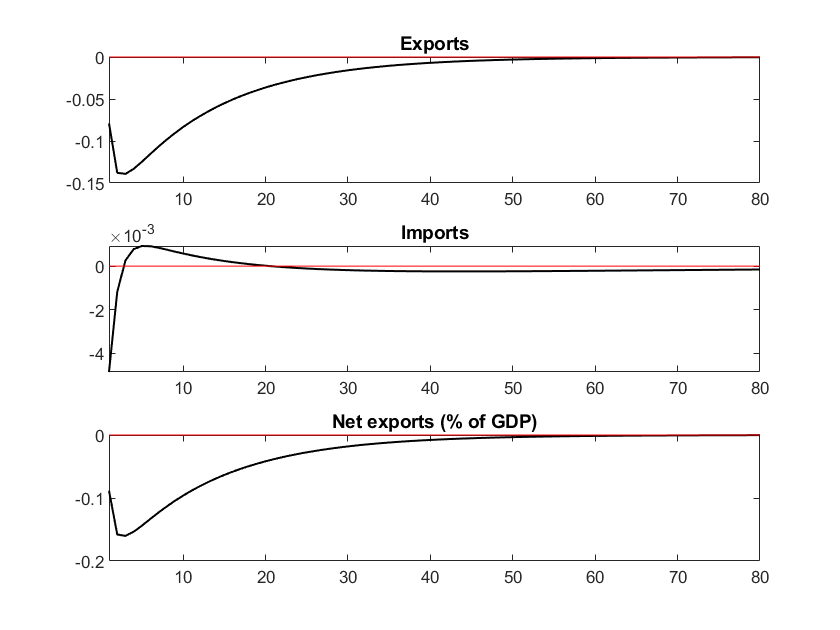
\includegraphics[width=1\textwidth]{C:/Users/mariu/Documents/Master_Thesis/Master_thesis/Pics_graphs/Simple_simulation_core.png}\\
\end{center}
\end{figure}

Figure \ref{Baseline Simulation} shows the impulse response functions of the health shock to exports, imports and net exports as a share of GDP. We see a strong drop in exports on impact. This is unsurprising since any negative change in health reduces productivity and labour supply directly. Both factors are direct components of the nation's output which equals exports as outlined earlier. In the second period after the shock , exports start to converge towards it's steady-state level based on the diminishing effects of the shock slowly increasing output. The model suggests the convergence to last up to 60 years. This is in line with estimates from \cite{ashraf2008does} which suggest health shocks on productivity to last around 50 years.\\
The effect on imports is different. On impact, imports decrease but by a smaller margin than the exports. That is because consumers want to smooth consumption which can on impact be achieved by increasing debt. That means imports drop less. Immediately after, imports increase and even surpass the steady-state level. Since labour supply and productivity start to coverge back to steady-state level, the gains of that are being distributed between paying back debt, higher consumption and more investment. Higher consumption and investment mean increased imports.\\
The trade balance is by definition the difference between exports and imports. It therefore follows the export's behaviour simply because the direct impact on exports is significantly stronger than the indirect impact on imports but on a wider amplitude incorporating the increased imports from period two onwards. The behaviour of other model variables of the home and foreign country is portrayed in table \ref{Baseline Simulation Extended} and \ref{Baseline Simulation Foreign} in the appendix. \\
If we were to believe this model as the true model, we would expect the empirical estimation to yield on impact negative coefficient of health for every dependent variable of interest exposed above. Empirical impulse response function might show statistical insignificance of health regressed on exports in the following two to three years and than significantly positive results. After the contemporaneous effect, the estimated coefficient for health should turn positive. All with a smaller coefficient, however. The coefficient of a health measure on trade balance is expected to behave as the estimated coefficient for health on exports.

\subsection{Expanded model}

The model so far has some oversimplified features. The assumption of one bundle of goods being exported automatically might be severly altering the simulation results. The fact of an exchange economy makes prices obsolete, adding a further criticism.\\
Therefore, I now model an economy following \cite{backus1992international}. Key feature is now a separated intermediate goods and final goods producer. Final goods can be produced by combining the foreign good and the home good. Intermediate production therefore produces for both markets. We have an bundle of exported goods and a bundle of non-exportables. Introduced prices allow us to leave the idea of an exchange economy behind. \\
The following section provides a concise, mathematical overview of the economic environment.

\subsubsection{The environment}

Generally, indexation is equivalent to previous. $t$ references the time, while there are two countries. Now, the $^{*}$ denotes the foreign country to avoid subscript confusion. Since it experiences the greatest changes to earlier, let me start by describing the production side of the economy.\\
The intermediate production is described by the usual Cobb-Douglas production function similar to above.
\begin{align}
a_t + a_t^* = A_t N_t^{1-\alpha} K_{t-1}^{\alpha} = f_t \\
b_t^* + b_t = A_t^* N_t^{*^{ 1-\alpha}} K_{t-1}^{*^{\alpha}} = f_t^*
\end{align}
here, $a_t$ is production of country one for it's home market while $a_t^*$ denotes production for the foreign market. Due to the symmetrical set-up, country two has the same production function with the difference that it produces good $b$. $b*$ denotes country two's need for locally produced goods and $b_t$ for the exports to country one. Per definition, this is equal to the imports of country one.
The intermediate goods are now used to produce the final good. This is commonly done by aggregating following \cite{armington1969theory}. Since the final good is non-tradeable, it represents the entire country's wealth. Intermediate production is not the wealth anymore because prices of imports and exports have to be taken into account. The final goods producer is therefore
\begin{align}
(\omega a_t^\theta + (1-\omega) b_t^\theta)^{\frac{\theta}{\theta-1}} \\
((1-\omega) a_t^{*^{\theta}} + \omega b_t^{*^{\theta}})^{\frac{\theta}{\theta-1}}
\end{align}

The prices will be explained in more detail later.\\
Since wealth has to be either consumed or invested, we arrive at the resource constraints
\begin{align}
K_t - (1-\delta)K_{t-1} + C_t = (\omega a_t^{\frac{\theta-1}{\theta}} + (1-\omega) b_t^{\frac{\theta-1}{\theta}})^{\frac{\theta}{\theta-1}} \\
K_t^* - (1-\delta)K_{t-1}^* + C^*_t= ((1-\omega) a_t^{*^{\frac{\theta-1}{\theta}}} + \omega b_t^{*^{\frac{\theta-1}{\theta}}})^{\frac{\theta}{\theta-1}}
\end{align}
$\omega$ represents the home bias. For reasons of simplicity and since it adds no substantial insights, debt is now dropped. Capital adjustment costs are being left out for the same reason.\\
Utility function, stochastic processes for productivity, labour and health remain as in the earlier model.

\subsubsection{Decentralized Solution}

Having the updated setting in mind, we can follow the same path as earlier. We optimize housholds consumption choice subject to the resource constraint as well as firms capital choice. That yields the following steady-state characterizing equations 
\begin{align}
\lambda_t = C_t^{\gamma-1} \\
\lambda_t^* = C_t^{*^{\gamma-1}}
\end{align}
(24) and (25) are the first order conditions of the household with respect to consumption. The intermediate producers optimize capital and face the optimal rental rate choice of (26) and (27). $f_t$ the total output of it.
\begin{align}
r_t = \frac{\alpha f_t}{k_{t-1}} \\
r_t^* = \frac{\alpha f_t^*}{k_{t-1}^*}
\end{align}
Solving the final good producers with respect to input factors $a$, $a^*$, $b$ and $b^*$ yields the demand functions. We solve for input prices $q_a$, $q_{a^*}$, $q_b$ and $q_{b^*}$ that can be red as demand functions.
\begin{align}
q_{a,t} = \omega a_{1,t}^{\theta-1} ((\omega a_{1, t}^{\frac{\theta-1}{\theta}} + (1- \omega) b_{1,t}^{\frac{\theta-1}{\theta}})^{\frac{\theta}{\theta-1} -1} \\
q_{b,t} = (1-\omega) b_{1,t}^{\theta-1} ((\omega a_{1,t}^{\frac{\theta-1}{\theta}} + (1-\omega) b_{1,t}^{\frac{\theta-1}{\theta}})^{\frac{\theta}{\theta-1} -1} \\
q_{a,t}^* = (1-\omega) a_{2,t}^{*^{\theta-1}} (((1-\omega) a_{2,t}^{*^{\frac{\theta-1}{\theta}}}+ \omega b_{2,t}^{*^{\frac{\theta-1}{\theta}}})^{\frac{\theta}{\theta-1} -1} \\
q_{b,t}^* = \omega b_{2,t}^{^*{\theta-1}} (((1-\omega) a_{2,t}^{*^{\frac{\theta-1}{\theta}}} + \omega b_{2,t}^{*{\frac{\theta-1}{\theta}}})^{\frac{\theta}{\theta-1}-1}
\end{align}
By transforming and combining, we obtain the well-known, slightly modified consumption Euler.
\begin{align}
\beta C_{t+1}^{\gamma-1} (q_{a,t+1} r_{t+1} + 1 - \delta)= C_t^{\gamma-1} \\
\beta C_{t+1}^{*^{\gamma-1}} (q_{b,t+1}^* r_{t+1}^* + 1 - \delta)= C_t^{*^{\gamma-1}} 
\end{align}
We observe that future consumption in terms of consumption today has to be adjusted for price changes, too. \\
The real exchange rate is defined as the value of home currency in terms of foreign currency.
\begin{align}
rer_t = \frac{qa_t}{qa_t^*} \\
rer_t^* = \frac{qa_t^*}{qa_t}
\end{align}
Lastly, the trade balance is now price adjusted such that
\begin{align}
nx_t = q_{a,t} a_t^* - q_{b,t} b_t \\
nx_t^* = q_{b,t}^* b_t^* - q_{a,t}^* a_t
\end{align}


\subsection{Simulation of the expanded model}

We can now turn to a simulation of the outlined, expanded model. All pervious parameters and initial values have been kept. The home bias $\omega$ is being determined at 0.9 from the dataset.\footnote{The home bias can be determined by solving the first-order condition for $\omega$. We apply some manipulations and obtain that \begin{align}
\frac{\omega}{1-\omega} = \frac{1 - \frac{b}{a + a^*}}{\frac{b}{a + a^*}}
\end{align}
with $\frac{b}{a + a^*}$ as the import to GDP ratio}
\cite{heathcote2002financial} provide an estimate for elasticity of substitution between foreign and home goods. While their estimation yields 0.9, today's research shows a broad range of estimation and ongoing discussion (\cite{feenstra2018search}). As pointed out by \cite{feenstra2018search}, any analysis including the Armington aggregator depends crucially on the $\theta$ parameter. However, to the best of my knowledge, there is no aggregated estimate for the countries considered in this study. Therefore, I decided to keep the parameter by  
\cite{heathcote2002financial}.\\
As mentioned perviously, second-order moments for the evaluation of the model are unsuitable at the moment. That is due to the unequal time horizon between theoretical simulation and real world data. Therefore, we should interpret simulation as a forecast while the first time periods can be used to test whether the general direction of the model works. \\
The simulation show a slightly different picture than the previous one. We can see in Figure \ref{Expanded Simulation} that exports behave in a similar fashion, however at a lesser extent. Since production is lower, good a becomes relatively scarce causing an increase in the price of it. That is because the intermediate goods complement each other leading to a reduced drop of exports.
\begin{figure}[!ht]
\begin{center}\caption{Expanded Simulation \label{Expanded Simulation}}
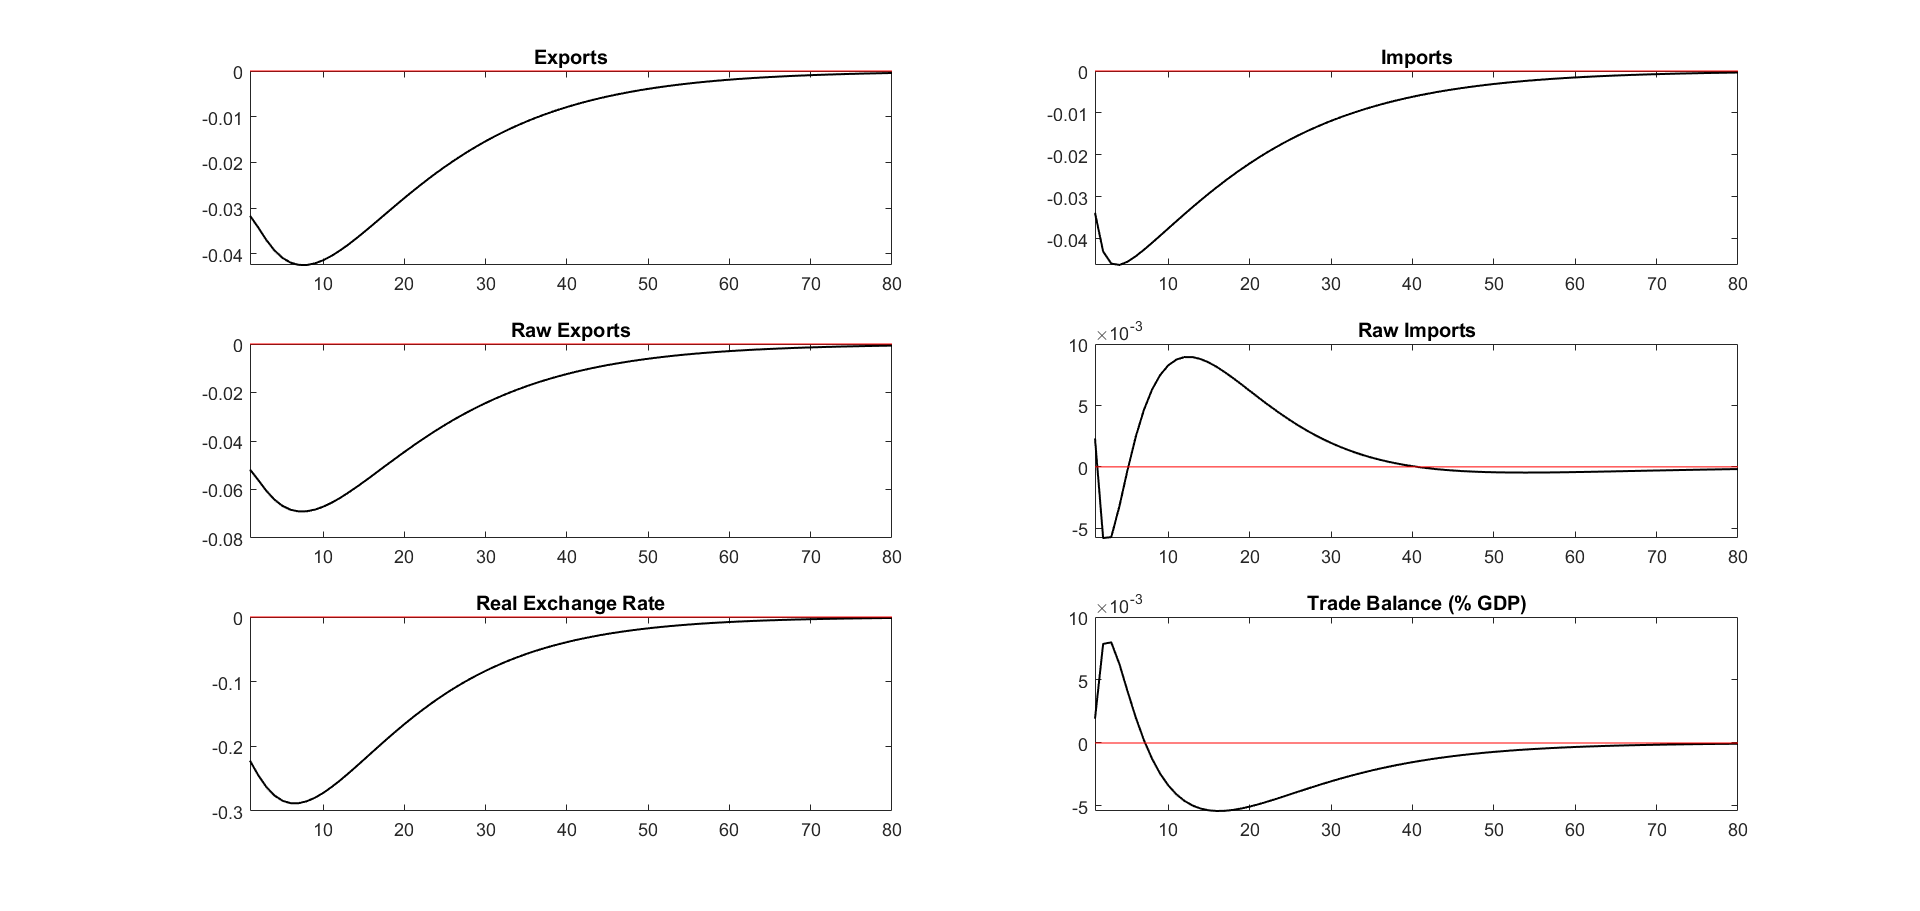
\includegraphics[width=1.1\textwidth]{C:/Users/mariu/Documents/Master_Thesis/Master_thesis/Pics_graphs/Simulation_expanded_1.png}\\
\end{center}
\end{figure}
While raw imports follow the trend of the simple model, the price-adjusted imports behave differently. This can be attributed to the price mechanism, too. The drop in prices of foreign-produced goods causes the real value of them to drop further than without price mechanism. The subsequent increase in imports is being consumed by the larger-in-margin and slower-in-recovering decline in foreign prices. \\
Lastly, the net exports first increase and than bounce into negativity. Later, it slowly converges back to zero. This suggests that the price-including impact of health shocks is larger on imports than on exports, at least on impact. Than as well, the convergence appears to happen faster for imports causing the negative sign of the trade balance.\footnote{Any further simulation results can be provided by the author}\\
Having simulated two different models, we have clear hypothesis and expectations for the empirical analysis. Firstly, strong and consistent negative effects on exports. Secondly, less strong and on impact consistently negative impacts on imports. Thridly, likely positive but potentially insignificant effects on the trade balance.

\section{Empirics}

\subsection{Regression design}

In order to find out where to start when doing the empirical analysis, we can turn to the simple benchmark model again. We saw there that the primary influence of health shocks are via the production function
\begin{align*}
Y_{i, t} = A_{i, t} N_{i, t}^{1 - \alpha} K_{i, t}^{\alpha}
\end{align*}
Afterwards, we take the logarithm to receive
\begin{align*}
\text{ln } Y_{i, t} = \text{ ln } A_{i, t} + (1 - \alpha) \text{ ln } N_{i, t} + \alpha \text{ ln } K_{i, t}
\end{align*}
Finally, we substitute a generalized version of (5)-(6) as well as (7)-(8) and collect terms.
\begin{align}
\text{ln } Y_{i, t} = (2 - \alpha)H_{i, t} + \rho^A \text{ln } A_{i, t-1} + (1 - \alpha) \rho^N \text{ln } N_{i, t-1} + \alpha \text{ln } K_{i, t}
\end{align}
Since production in the simple model equals exports, we can see (20) as the benchmark regression to determine the impact of health shocks on exports. $H_{i, t}$ has the pre-factor $(2 - \alpha)$ originating in the idea that health shocks hit productivity with an elasticity of one while the same shock to labour affects overall exports only as much as labour is used in production. Logically, the exponent has to be positive meaning better health increases production and exports. \\
Since $H_{i, t}$ follows a stochastic process in the model and itself depends on various determinants, an instrumental variables approach seems natural. If we are able to identify a shock to health, we can use the shock to predict a health measure and subsequently test for the impact on exports, imports and trade balance. \\

\subsection{The ideal experiment}
In an ideal setting, one would like to have a comprehensive administrative dataset at the individual level. This should at least state whether a person had Ebola and demographic statistics such as age. Additionally we would need firm data on exports and imports or, in case of self-employment the individual's trading data. Lastly, we would have to link each person not self-employed to its employer. With all this information we are able to construct a micro-level analysis and see how much firms' exports and imports are dampened by the share of workers being infected. If we were to have data on when exactly a person is infected and when she stops working we would be able to separate productivity from labour supply effects. Further, we would see how prices of domestically produced goods develop and could check if the price mechanism truly works as designed. Overall, we would be able to track the consequences perfectly and disentangel different effects going on simultaneously.\\
Unsurprisingly, there is a lack of data. The most glaring lack is demographic data. Surveys, unfourtunately, are not conducted in sufficiently small time intervals. Moreover, firm-level data is missing, too. \\
Luckily, country-level data are complete and available. Therefore, we have to trade the heterogeneity occurring on more filigree levels with having data at all. This is far from perfect but allows to continue investigating.\\

\subsection{Data}

\subsubsection{Measuring Ebola}

Generally, researchers consulted the Standard Inflammatory Response (SIR) model when assessing epidemics. It has been used in epidemiology since it's discovery by \cite{kermack1927contribution}. Nowadays, it is the  standard model in describing the transmission dynamics of epidemic diseases. It is not only used in epidemiology, as in \cite{shulgin1998pulse} but also in mathematics (\cite{mccluskey2010complete})  and ecology (\cite{bjornstad2002dynamics}). In economics, the model is employed in \cite{hansen2017preventing}. \\
Generally, the model separates individuals into either \textit{Suspectible}, \textit{Infected} or \textit{Recovered}. Individuals have the chance to remain in the same category or change to a different category at the beginning of each new period. Death can potentially occur at any group however with different probabilities. Additionally, there is a certain amount of new people born every period entering as \textit{Suspectibles}. Figure \ref{Schematic SIR} puts the mechanics in a space graph following the representation of \cite{bhattacharya2013health}.

\begin{figure}[!ht]
\begin{center}\caption{ Schematic SIR \label{Schematic SIR}}
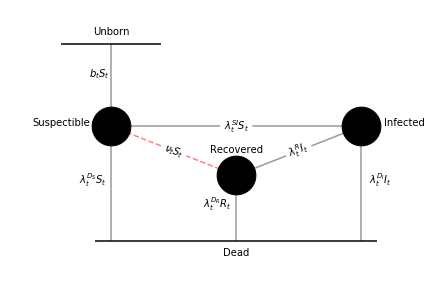
\includegraphics[width=0.8\textwidth]{C:/Users/mariu/Documents/Master_Thesis/Master_thesis/Pics_graphs/SIR.png}\\
\smallskip {\footnotesize Author's own work}
\end{center}
\end{figure}

$b_t S_t$ equals the number of all births in time $t$, with $b_t$ being the birth rate and $S_t$ the number of non-infected individuals, the \textit{Suspectibles} that are not immune. $\lambda_t^{D_S} S_t$ represents the amount of non-immune people dying of other causes than the disease of interest. All immune people, the \textit{Recovered}, dying in $t$ are captured by $\lambda_t^{R_S} R_t$. This group consists of all people being vaccinated $\nu_t S_t$ and those having recovered from the disease $\lambda_t^{R} I_t$ with the recovery rate $\lambda_t^{R}$ . The total number of new infection is given by $\lambda_t^{SI} S_t$. The death toll of the disease is stated with $\lambda_t^{D_I} I_t$. \\
To model the Ebola epidemic, the standard model needs some minor adjustments. Hereby, I follow \cite{hansen2017preventing} in modelling the SIR model and discretizing the model to ease the transition to the empirical estimation. \\
Firstly, I consider the \textit{Suspectibles}. This pool of non-infected, non-immunized person develops according to

\begin{align*}
S_{t+1} = S_t + b (S_t + R_t) - \lambda_t^{SI} S_t - \lambda_t^{D_S} S_t
\end{align*}

where $b$ is a exogenously given birth rate. New-borns are automatically entering as suspectibles. This is a simplifying assumption since \cite{dornemann2017first} give proof of babies born to Ebola-virus positive women inheriting the virus. However, it does not alter the results justifying this simplification. Further, I assume that infected women are not able to give birth. This, as well, is not true but due to limited cases not changing the findings (\cite{baggi2014management}). $\lambda_t^{SI}$ is the infection rate of Ebola and $\lambda_t^{D_S}$ represents the exogenous death rate due to other causes than Ebola. \\

\begin{align*}
R_{t+1} = R_t + \lambda_t^{R} I_t - \lambda_t^{D_R} R_t
\end{align*}

explains the motion of recovered agents with $\lambda_t^{R}$ being the recovery rate. $\lambda_t^{D_R}$ describes the death rate of people having recovered from Ebola. This is exogenously given and may or may not differ from $\lambda_t^{D_S}$. $\nu_t R_t \equiv 0$, since there is no vaccine for Ebola at the time being, although progress towards it has been made (\cite{ledgerwood2017chimpanzee}).\\
The remaining group of the population is the infected. In essence, the infected follow

\begin{align*}
I_{t+1} = I_t + \lambda_t^{SI} S_t - \lambda_t^{Eb} I_t - \lambda_t^{I} R_t
\end{align*}

the infection rate $\lambda_t^{SI}$ is exogenously given, as is $\lambda_t^{Eb}$, the Ebola death rate among infected. Unsurprisingly, the rate of recovery for Ebola $\lambda_t^{I}$ is exogenous, too. \\
With this in mind we can formulate a Ebola-related case prevalence rate.

\begin{align*}
CP_{t}^{Eb} = \frac{I_t}{P_t} = \frac{I_t}{S_t + R_t + I_t} \\
\end{align*} 

to solve for the stochastic solution yields

\begin{align*}
CP_t = \frac{(1 - \lambda^{Eb}_{t-1})I_{t-1} + \lambda_{t-1}^{SI} S_{t-1} }{(1+b-\lambda_{t-1}^{DS})S_{t-1} + (1+b-\lambda_{t-1}^{DR})R_{t-1} + (1 - \lambda_{t-1}^{R}- \lambda_{t-1}^{Eb})I_{t-1}}
\end{align*}
where all parameters are assumed exogenous.\\
There are several reasons for doing so. Firstly, effects such as changes in consumer behaviour do not have to be associated to deaths but could be  as well associated to the infection whether deadly or not. Secondly, the number of workers is defined as the uninfected portion of the population. So capturing the mortality rate would ignore the number of infected unable to work. Thirdly, as long as recovery rate and death rate of the disease are constant the case prevalence and mortality rate will be highly correlated. And indeed, the correlation coefficient is approximately $0.7$. Lastly and maybe most importantly, we need the prevalence rate to ensure comparability in the panel set-up the Ebola outbreak left us with. A simple use of infected would ignore the impact a small number of infected has on a overall very small population. \\

Data on Ebola cases and deaths are from the situation report by the \cite{whoebola} and occur in a high frequency which has been exploited by studies such as \cite{gonzalez2017epidemics} or \cite{althaus2014estimating}. The lack of high-frequency data in the areas of population and trade however, force me to aggregate to a yearly level losing heterogeneity across time. While Ebola cases and deaths are not only the most intuitive measure but also of reliable quality, it might make sense to expand the set of measurements.\\
Big data has helped epidemic research substanstially in predicting outbreaks of different diseases, consider \cite{ginsberg2009detecting} as an example, as well as their surveilling (e.g. \cite{chan2011using}).
I consider the number of New York Times Articles about Ebola in a given country in a given year as an additional measurement. Even though it can't be literally defined as big data it shows remarkable similarities as shown in figure \ref{NYT and Google}, where both number are scaled to be between 100 and 0 with 100 being the month with the most queries/articles.

\begin{figure}[!ht]
\begin{center}\caption{ NYT and Google \label{NYT and Google}}
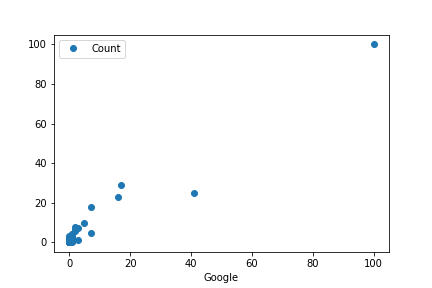
\includegraphics[width=0.6\textwidth]{C:/Users/mariu/Documents/Master_Thesis/Master_thesis/Pics_graphs/mytable.png}\\
\end{center}
\end{figure}

If the prevalence rate's parameters were not be exogenously given but depending on other factors, the other measurement would have an advantage. Albeit, at the time of the outbreak, $R_t$ and $I_t$ are clearly zero and we can control for the \textit{suspectibles} - they equal the overall population - parameters can be changed in second period by potentially unobserved variables. The alternative measure does not exhibit this pattern. Naturally, we expect a high, statistical significant correlation with the number of Ebola cases and yet a respectable distance to a perfect correlation represented by 1. The sample correlation with 0.633 seems to confirm the intuition. \\
On the other hand, there are disadvantages when using this measure.
Firstly, we assume that the NYT has no inherent bias towards certain countries in the study. This is part of the reason for chosing the NYT since countries with a colonial link might show higher temptation to report on the former colony. The United States do not have a past a colonizer but regardless might exhibit a bias towards the English-speaking countries in the sample, in particular Sierra-Leone and Liberia. \\
Secondly, we might overestimate foreign response if the interest of the NYT in Ebola is higher than of the representative consumer. Similarily, we underestimate if the interest of the newspaper abates while the household is still concerend about Ebola. An example could be that a mayor event in a different foreign country takes up the space of limited lines in the newspaper.\\
Lastly, we arguably worry about an US newspaper representing the entirty of global demand we is likely to be very heterogeneous and only coincidetally on average similar if we're refusing to assume a preference shaping role of the US. \\
Table \ref{Ebola Measures} shows a summary of the discussed measures.

\begin{table}[htbp]\centering \caption{Ebola Masures \label{Ebola Measures}}
\begin{tabular}{l c c c c c}\hline\hline
\multicolumn{1}{c}{\textbf{Variable}} & \textbf{Mean}
 & \textbf{Std. Dev.}& \textbf{Min.} &  \textbf{Max.} & \textbf{N}\\ \hline
Ebola cases & 84.091 & 815.583 & 0 & 14122 & 680 \\
Ebola deaths & 12.238 & 163.731 & 0 & 2536 & 680 \\
Ebola articles & 2.568 & 29.123 & 0 & 527 & 680 \\
\hline\end{tabular}
\end{table}

Since this study focuses on the 2014 Ebola outbreak only, outbreaks in different countries at previous or following years are being ignored. Prime example is the 2000-2001 outbreak in Uganda. This is potentially problematic as it can violate the assumption of common Pre-Trends. Further, countries with limited or local cases in 2014 such as Senegal or Nigeria are equally ignored. If these limited outbreaks do indeed have an impact on the mortality rate, it causes the results to be biased. The country-pair structure of the data allows us to exclude relevant observations and effectively correct for any potential bias.

\subsubsection{Measuring Health}

When it comes to measuring health, there are two obvious choices occurring widely in the literature, mortality rate and life expectancy. They are closely related since life expectancy is defined as
\begin{align} 
LE(n,x) = 1 - e^{n*m(n,x)}
\end{align}
where $m(n,x)$ is the age-specific mortality rate starting at age $x$ to age $n + x$. Therefore, a considerable change occurs mostly at interpretation of any results. \\
Generally, the literature has been looking at life expectancy at birth as a measure for health, for instance consider \cite{bloom2018health}, \cite{acemoglu2007disease} or \cite{bloom2014disease}. This seems to be a sensitive measure for long term if the overall objective is to collect all possible effects happening during a lifetime. For instance, it captures reduced child mortality as well as better medication for HIV which can prolong live at an adult stage as well. However, trends across countries and age group can differ substantially as highlighted by \cite{mcmichael2004mortality}. Given this heterogeneity in trends since adults are more likely to be infected and infants or children do not transmit health outcomes in economic terms at the same rate. Therefore, I will use adult mortality rate as a baseline result, since it excludes changes in mortality due to improvements in survival rate during life childbirth. \\
Yet, in a more dynamic perspective it might be that less stress of the mother while bearing the child could potentially increase productivity and education, as the fetal origin hypothesis suggests\footnote{ \cite{almond2011killing} give a more detailed introduction to this theory and further provide a cohesive literature review.}. In addition, \cite{norman2012long} point out the severe consequences of a diverse range of mental and physical abuses can have on a person's live. These include a higher suicide rate, drug use and mental disorder. \\
Table\ref{Main Health Measures} summarizes these measures.

\begin{table}[htbp]\centering \caption{Main Health Measures \label{Main Health Measures}}
\begin{tabular}{l c c c c c}\hline\hline
\multicolumn{1}{c}{\textbf{Variable}} & \textbf{Mean}
 & \textbf{Std. Dev.}& \textbf{Min.} &  \textbf{Max.} & \textbf{N}\\ \hline
Adult mortality rate & 339.46 & 97.36 & 185 & 637 & 680\\
Life expectancy & 56.20 & 5.52 & 39.8 & 68.7 & 680 \\
\hline\end{tabular}
\end{table}

Life expectancy and mortality data are taken from the \cite{whostatistics} and their Global Health Workforce Statistics. One might notice the high number of observations. This originates in the structure of the trade data, which are measured in country pairs. A more careful explanation of the reasons to measure trade with country-pairs will be provided later. \\
Further measures could be Anemia, neonatal mortality rate, infant mortality or birth weight (\cite{weil2014health}) or even include crude data such as death rate. These additional measures for health are displayed in Table \ref{Appendix - Data}, panel A, in the appendix. These additional data are taken from \cite{wdi}.

\subsubsection{Trade Measures}

The previos sections have already hinted that I will be using country-pair trade data. The chapters also provided some reasons for doing so. We can exclude direct neighbours to Ebola affected countries and therefore control for spillover effects, we can omit countries having had limited outbreak and subsequently exclude them to see for any biased estimates and we can omit countries with periods of any sort of epidemic, Ebola or other, potentially violating the common trends assumption. \\

\begin{table}[htbp]\centering \caption{Trade Masures \label{Trade Measures}}
\begin{tabular}{l c c c c c}\hline\hline
\multicolumn{6}{c}{Trade Data}\\ \\ \hline
\multicolumn{1}{c}{\textbf{Variable}} & \textbf{Mean}
 & \textbf{Std. Dev.}& \textbf{Min.} &  \textbf{Max.} & \textbf{N}\\ \hline
Imports (\% of GDP) & 0.014 & 0.173 & 0 & 14.825 & 63537\\
Exports (\% of GDP) & 0.006 & 0.07 & 0 & 3.669 & 57261\\
Trade Balance (\% of GDP) & -0.004 & 0.087 & -5.22 & 2.597 & 83428\\
\hline\end{tabular}
\end{table}
Naturally, the gravity approach increases the amount of observations drastically. In order to normalize the the crude export and import values, I divded each by the country's corresponding GDP value so that terms relative to GDP are obtained. The directions of trade dataset by the \cite{imfdot} provides the bilateral trade data. \\
During the course of this investigation, I employ several control variables. These will be explained carefully by the time of their introduction. However, an overview over all controls as well as the crude trade data summary is given in Table \ref{Appendix - Data} in the Appendix.

\subsection{First Stage}

Empirical estimation is difficult. This is mainly because causal relationships can not only work from health to trade, as I try to investigate, but obviously in the reverse order as well, as emphasized in section II. Additionally, one has to worry about a third, omitted variable that drives both trends simultaneously. Economic growth could be such a driver. Therefore, I suggest to employ a natural experiment to solve the issue of identification. The 2014 Ebola outbreak in Westafrica, in particular in Guinea, Liberia and Sierra-Leone, is such which allows me to employ a difference-in-differences (DiD) approach.
The baseline estimation regression is

\begin{align}
H_{it} =  \beta Z_{it} +  Q_{it}'\gamma + \pi_{it} + \alpha_i + \gamma_t + \epsilon_{it}
\end{align}
where $i$ indexes the country-pairs and $t$ time. $Y_{it}$ captures the outcome variable measuring health, age-adjusted adult mortality rate, while $Z_{it}$ is our variable of interest - Ebola - with $\beta$ the corresponding coefficient. Both are scalars at time $t$ for unit $i$. The vector $Q_{it}$ is of rank $K \times 1$ with $K$ being the number of controls for each unit at each time added to the regression. $\gamma_t$ controls for differences across years common to all states and $\alpha_i$ for differences across countries ocurring to all states. $\pi_{it}$ is a country-pair specific, linear trend over time. The idiosyncratic error term is represented by $\epsilon_{it}$. \\
However, reasoning is mandatory since a natural experiment in the sense of a DiD requires common trends between treatment and control group prior to the treatment. Hereby arises the first question of how to select a control group. This is not a trivial task since simply taking all other countries as control group certainly forces the common trends to fail. To begin with, we need to ensure that the disease environment is approximately equal across sample countries. If there was a significant difference in the probabilty of an epidemic due to environmental circumstances such as temperature or encroachment to forest (\cite{alexander2015factors}), we would not have a random assignment of the treatment making use of policy evaluation unsuitable.\\
Secondly, a functioning health infrastructure can significantly limit the likelihood of an epidemic outbreak (compare a hypothetical outbreak in the US vs. Guinea). That being said, I exclude all countries that are grouped higher than a low-income country by the World Bank at the start of the sample in the year 2000 since all three treatment countries are grouped as such. The control group is composed of the union of the two criteria mentioned.\\
Having established a solid control group necessarily leads to the question of whether the common trend assumption actually holds. There are several anecdotal arguments for this. Primarily, the history of the Ebola virus. 2014 was the first outbreak of Ebola in any of the affected countries. Additionally, it was the first epidemic outbreak of Ebola ever and even the emergency experts of MSF and WHO were surprised and did not expect Ebola in these countries, as has been outlined in section III.\\
Lastly, even though there has been research indicating that Westafrica should be considered potentially vulnerable, no public health official in Liberia knew of a potential danger neither the epidemic scale, as claimed by \cite{ebola2015nyt} in a 2015 New York Times (NYT) opinion piece.

\begin{figure}[!ht]
\begin{center}\caption{ Number of articles about Ebola in the NYT \label{Number of articles about Ebola in the NYT}}
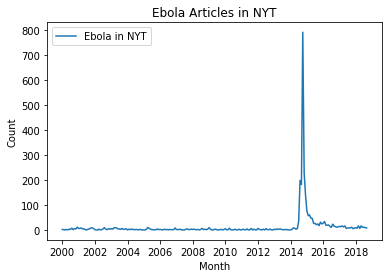
\includegraphics[width=0.6\textwidth]{C:/Users/mariu/Documents/Master_Thesis/Master_thesis/Pics_graphs/Ebola_nyt_python.png}\\
\end{center}
\end{figure}

Moreover, it is highly unlikely that the general public knew much about Ebola at all. Figure \ref{Number of articles about Ebola in the NYT} shows the articles in the NYT mentioning Ebola at least once. Assuming that the NYT represents an (educated) population and reflects interests and priorities of a society, we clearly see that Ebola has not been a particular focus before the 2014 outbreak even though there have been several smaller outbreaks in the Congos or Gabon, amongst others, since 2000. Further, Google search query trends show a similar behaviour on large (see Fig. \ref{NYT and Google}). All in all, I think this is strong evidence of why there has been no adjustment of health behaviour with respect to Ebola prior to the treatment thereby establishing the common trend assumption. Anecdotal evidence does not substitute a thorough statistical analysis since pre-trends might be there, regardless. \\
The following section provides this analysis whether the common trends assumption can be believed to hold.

\subsubsection{Event Study}

Before we turn to performance of the DiD estimator, a closer look on the common trends assumption is imperative. Commonly, this is done by graphical inspection. Figure \ref{Pre-trends} shows how the averages of treatment and control group evolve around the intervention. Both are standardized around the control group at the year 2004.

\begin{figure}[!ht]
\begin{center}\caption{Pre-trends \label{Pre-trends}}
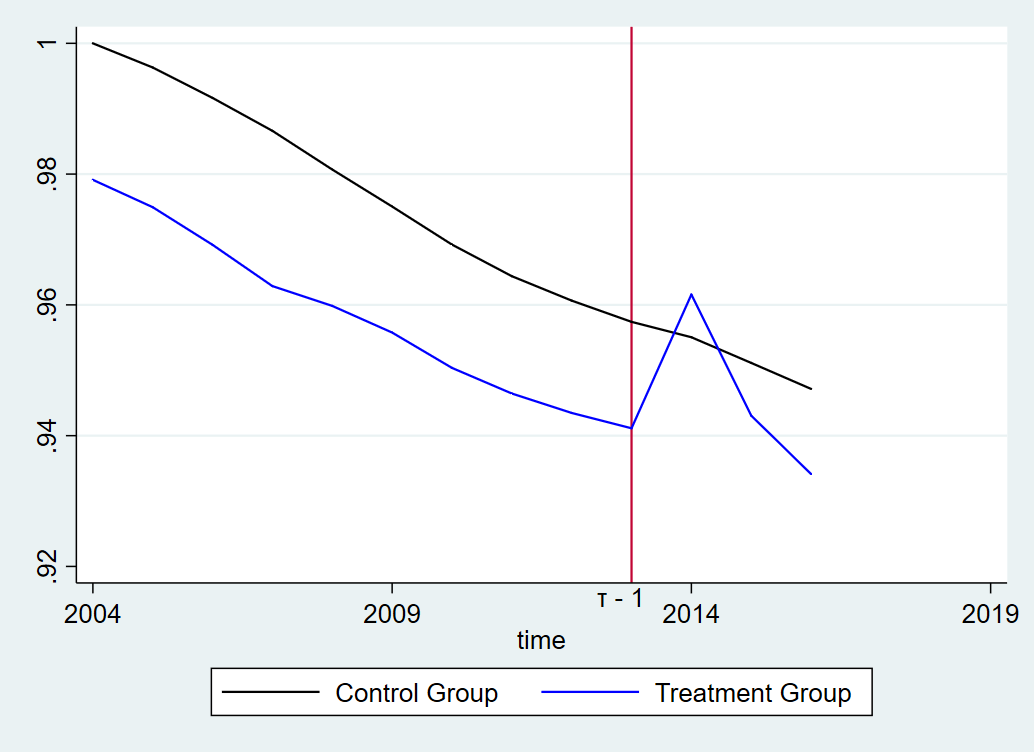
\includegraphics[width=0.8\textwidth]{C:/Users/mariu/Documents/Master_Thesis/Master_thesis/Pics_graphs/Averages_pre_trends.png}\\
\end{center}
\end{figure}

By eyeballing, we fail to see differences in pre-trends of treatment and control group. This finding gives confidence in the common trends assumption. Due to several treatment groups as well as several control variables, averages may be misleading surpressing important heterogeneity in the data. The common approach in the literature to solve the problem of multiple entries or treatment units are so called event studies, as pioneered by \cite{bertrand2004much} while \cite{freyal2018pre} and
\cite{borusyak2017revisiting} provide recent discussion about pre-trend diagnostics. \\
The intuition is to simulate the same shock, holding controls equal, in every year before and after the actual shock at $\tau$. If there are significant effects in every year prior to the intervention we would interpret this as a constant difference between control and treatment group regardless of the intervention and the common trends assumption is unlikely to hold. The mathematical representation following \cite{pischke2005empirical} can be seen in equation (44).

\begin{align}
H_{it} =  \sum_{j=-m}^q \beta_j Z_{it}(t = \tau + j) + \alpha_i + \gamma_t + \epsilon_{it}
\end{align}

where $k$ is the time of the actual treatment, $m$ representing leads, simulating treatment prior to the real treatment, and $q$ lags, simulating treatment after the original one. In mathematical terms we need at least that $\beta_j = 0 \ \forall \ j < 0$ holds. While $\beta_j \neq 0 \ \forall \ j > 0$ is allowed since these can be interpreted as response coefficients over time such that $\sum_{j= \tau}^q \beta_j Z_{it}(t = \tau + j)$ represents the accumulated effect of the shock until $q$. \\
Figure \ref{Event Study} shows the estimated coefficients for the Ebola "event" in 2014 with $-m$ equalling the year 2000 and $q = 2016$. Therefore, I include a total of 14 pre-treatment and 2 post-treatment periods. The estimation also includes a country-specific linear trend as it does in the baseline results which coefficient is not reported in the graph. Yet, the trend coefficient as well as more detailed results can be found in the Appendix Table \ref{Appendix - Event Study}. Any year $10 \leqslant j \leqslant 14 $ is grouped together as one estimand. By convention, the pre-treatment year $\tau - 1$ is used as standardization factor.

\begin{figure}[!ht]
\begin{center}\caption{Event Study \label{Event Study}}
\includegraphics[width=0.8\textwidth]{C:/Users/mariu/Documents/Master_Thesis/Master_thesis/Pics_graphs/Event_study.png}\\
\end{center}
\end{figure}

Each y-line represents a different event before or after the outbreak $\tau$ in the form of a coefficient in the regression (25) . The width of each estimate is the 95 \% confidence interval. We observe a highly, statistical significant coefficient at time $\tau$ and declining  estimation in magnitude for the following two periods which should not come as a surprise given that severity of the Virus dropped and international efforts became more efficient. Regardless, they still exhibit some statistical significance.\\
Within the pre-treatment periods are ten placebos that are statistically insignificant at the 5\% level which is what would expect and gives confidence in the common trend assumption. When being more thorough in including the pre-event years by including all individually, the coefficient for $\tau - 11$ becomes significant. All others remain insignificant. This gives rise to some concern regarding parallel trends. Hereby it needs to notice that remaining coefficients and confidence barely change. Therefore, it appears to be a unrelated event rather than a systematic violation. Appendix figure \ref{Event Study Robustness} shows the results graphically. \cite{freyal2018pre} suggest to include an observable covariable that is highly correlated to the pre-trend and the outcome variable to solve pre-trends. If we are to believe that the statistical significance of $\tau - 11$ is a violation of parallel trends we would need to find a covariable that is unexpected before and after the year 2003. Despite the ocurring proximity to a shock, I was unable to detect an event that could justify such a behaviour. Subsequently, I fail to include an appropriate control variable for $\tau - 11$.\\
Even given the concern raised just earlier, the common trend assumption seems to hold beyond a reasonable level of doubt because there is no systemic difference between both groups. The following subsection turns towards the estimated results of the intervention.

\subsubsection{Baseline results}

As explained earlier, the regression to estimate the impact of the ebola outbreak on health contains the variable of interest, a linear country-specific trend and fixed effects for time and country-pairs.\\
The results of this baseline regression can be seen in Table \ref{Baseline results}. Column I uses the prevalence of Ebola cases as a measure while Column II uses the number of Ebola articles.

\begin{center}
\begin{table}[htbp]\centering  \caption{Baseline results \label{Baseline results}}
\begin{tabular}{lcc} \hline
 & (I) & (II) \\
Dependent Variable & \multicolumn{2}{c}{Log Adult Mortality Rate} \\ \hline
\vspace{4pt} & \begin{footnotesize}\end{footnotesize} & \begin{footnotesize}\end{footnotesize} \\
Log Prevalence Rate & 0.9716*** &  \\
\vspace{4pt} & \begin{footnotesize}(0.3169)\end{footnotesize} & \begin{footnotesize}\end{footnotesize} \\
Log Ebola Articles &  & 0.0203*** \\
 & \begin{footnotesize}\end{footnotesize} & \begin{footnotesize}(0.00389)\end{footnotesize} \\
\vspace{4pt} & \begin{footnotesize}\end{footnotesize} & \begin{footnotesize}\end{footnotesize} \\
Linear Trend & -0.0236*** & -0.0238*** \\
\vspace{4pt} & \begin{footnotesize}(0.00267)\end{footnotesize} & \begin{footnotesize}(0.00270)\end{footnotesize} \\
Observations & 124,117 & 124,117 \\
$R^2$ & 0.633 & 0.635 \\
Number of country-pairs & 7,301 & 7,301 \\
Country-pair FE & Yes & Yes \\
Year FE & Yes & Yes \\
Cluster level & Country pair & Country pair \\
F-statistic & 39.60 & 69.58 \\ \hline
\multicolumn{3}{c}{\begin{footnotesize} \textit{Log Prevalence Rate} is the log of the number of infected divided by the total population \end{footnotesize} }\\
\multicolumn{3}{c}{\begin{footnotesize} \textit{Log Ebola Articles} is the log of the number NYT articles about Ebola and a country \end{footnotesize} }\\
\multicolumn{3}{c}{\begin{footnotesize} Clustered standard errors in parentheses. \end{footnotesize} }\\
\multicolumn{3}{c}{\begin{footnotesize} *** p$<$0.01, ** p$<$0.05, * p$<$0.1\end{footnotesize}} \\
\end{tabular}
\end{table}
\end{center}
In both cases, we can see strongly statistcally significant results. In column (I), an increase in the ratio of Ebola infected to the entire population by 1 \% leads to an approximate increase in the mortality rate by 0.97\% keeping everything else constant. In other terms, there are an additional 97 out of 10000 adult individuals to die before reaching the age of 60 or an average adult individual has a 0.97 \% higher probability of dying before reaching the age of sixty due to Ebola. \\
The alternative specification for Ebola has a slightly different interpretation. We associate an 1\% increase of Ebola-related articles and the particular countries with an increase of approximately 0.02\% in mortality rates. In a standard interpretation this implies that an additional 20.3 out of 10,000 adult persons will die before reaching the age of 60 when the number of articles increase by 10\%. Maybe even more intuitive, the 1\% increase in Ebola-related articles would be associated with the average person having a 0.203\% higher probability of dying before turning 60. \\
On a first glance, these results seem to be quite separated from each other. However, one needs to keep in mind that the increased chance of dying prognosed by the estimated coefficients covers a 45-year-long time period since the individual is assumed to be 15 in the \cite{whostatistics} data structure.\\
Lastly, the linear, country-specific trend is statistically significant at all common levels of significance indicating the initial presence of a random walk. \\
When performing the regression of health, measured on a national basis, and Ebola, measured on a national level, with country-pair data, the coefficient might be bias due to unequal weighting. For instance, if country A reports all health and trading data and at the same time country B all health but only one trading-pair data this might create artificial weights on this particular trading-pair. Subsequently, we would see a predominance of the effect in a certain set of countries-pairs. \\
We then estimate with is equal to before but now $i$ being the index for countries and not country-pairs.
\begin{align}
H_{it} =  \beta Z_{it} +  Q_{it}'\gamma + \pi_{it} + \alpha_i + \gamma_t + \epsilon_{it}
\end{align}

A similar coefficient and standard errors give confidence in the initial baseline results. 

\begin{table}[htbp] \centering \caption{Collapsed Baseline \label{Collapsed Baseline}}
\begin{tabular}{lcc} \hline
 & (1) & (2) \\
Dependent Variable & \multicolumn{2}{c}{Log Adult Mortality Rate} \\ \hline
\vspace{4pt} & \begin{footnotesize}\end{footnotesize} & \begin{footnotesize}\end{footnotesize} \\
Log Prevalence Rate & 1.296** &  \\
\vspace{4pt} & \begin{footnotesize}(0.597)\end{footnotesize} & \begin{footnotesize}\end{footnotesize} \\
Log Ebola Articles &  & 0.0217*** \\
 & \begin{footnotesize}\end{footnotesize} & \begin{footnotesize}(0.0055)\end{footnotesize} \\
\vspace{4pt} & \begin{footnotesize}\end{footnotesize} & \begin{footnotesize}\end{footnotesize} \\
Linear Trend & -0.0229*** & -0.0231*** \\
\vspace{4pt} & \begin{footnotesize}(0.0025)\end{footnotesize} & \begin{footnotesize}(0.0025)\end{footnotesize} \\
Observations & 680 & 680 \\
$R^2$ & 0.628 & 0.629 \\
Country FE & Yes & Yes \\
Year FE & Yes & Yes \\
Cluster & Country & Country \\
F-statistic & 42.04 & 47.37 \\
No. clusters & 40 & 40 \\ \hline
\multicolumn{3}{c}{\begin{footnotesize} \textit{Log Prevalence Rate} is the log of the number of infected divided by the total population \end{footnotesize} }\\
\multicolumn{3}{c}{\begin{footnotesize} \textit{Log Ebola Articles} is the log of the number NYT articles about Ebola and a country \end{footnotesize} }\\
\multicolumn{3}{c}{\begin{footnotesize} Clustered standard errors in parentheses. \end{footnotesize} }\\
\multicolumn{3}{c}{\begin{footnotesize} *** p$<$0.01, ** p$<$0.05, * p$<$0.1\end{footnotesize}} \\
\end{tabular}
\end{table}

When comparing Table \ref{Baseline results} to Table \ref{Collapsed Baseline}, we observe plentiful similarities. Statistical explanatory power is almost equal with the expection of the case prevalence being significant only at the 5 \% level. The coefficient of the case prevalence itself is slightly larger but well within the range of estimates following in the next section. The alternative specification does not differ in terms of statistical significance and the coefficient changes only at the third digit. Overall, the results give the impression that the potential weighting bias does not appear to be severe in size. Therefore, I proceed by using the country-pair specification. \\
Yet, the lack of control variables included imposes a threat to the consistenty of the OLS results known as the omitted variable bias. The following subsection will deal with this problem.

\subsubsection{Control Variables}

In the framework of DiD, we care about omitted variables for mainly two reasons. First, a control variable that correlates with the treatment variable causing an inconsistent estimate of the treatment effect. Secondly, in existence of unit-specific trends the common trend assumption could be violated. By including a control variable that captures precisely these unit-specfic trends, the common trend assumption could be restored. While the second concern doesn't not seem to pose any particular threat to the validity, at least on the basis of the event study performed earlier, the first concern might be problematic.\\
Unsurprisingly, finding and including a cohesive list of possible confounders is not an easy task. A vast body of literature trying to determine predictors of mortality exists already. Nice overviews are given by \cite{cutler2006determinants}, \cite{soares2007determinants} and \cite{arcaya2015inequalities} albeit with different focusses. Additionally, many determinants of health inequalities happen on an individual level. Examples include but do not constrain to stress, social inclusion and 
maternal stress during pregnancy (\cite{thoits2010stress}, \cite{cohen2004social} and \cite{almond2011killing}). These are hard to measure, even harder to aggregate and overall more likely to explain within-country variations rather than variations between countries. \\
Notwithstanding, there are some aggregated measures that can help to reduce the risk of inconsistent estimated due to omitted variable bias. \cite{cutler2006determinants}, for instance, argue that urbanization initially increases mortality rates due to the facilitated spread of diseases. In arguing that public health should be considered as a determinante, they follow \cite{preston1975changing}. The key argument is that higher income alone does not suffice to explain the historic reduction since countries would in return follow the Preston curve which is not matched by the data. Instead, public investments in sanitation, filtering water as well as setting up vaccination campaigns were essential. Another point by \cite{cutler2006determinants} is improved nourishment. Intuitively, a better-fed erson has a lower propensity to get sick and at the same a higher likelihood to recover faster.\\
Some more potential confounders are found in \cite{marmot2005social}. The author evaluate that wealth and inequality are important factors to consider when investigating health inequalities. While the data availability for inequality in 2014/2015 is not perfect yet and therefore not ready to be included, wealth data can be included. More recently, the internet has changed health behaviour of patients and doctors significantly (\cite{cook2008internet}). Therefore, I include the percent of internet accesses as an additional control variable.\\
Lastly, I capture any confounding effect of the most pressing diseases by including HIV prevalence, Tuberculosis cases and some others. Hereby, I follow the \textit{Global Burden of Disease Study} by \cite{lozano2012global}. Further, I considered including education but a growing amount of literature fails to confirm education as a determinant for adult health outcomes (\cite{clark2013effect} or \cite{meghir2018education}).\\
Generally, I organize the adding of control variable Table \ref{Control results} threepartly. First, control variables following the established literature are included (columns I and II). Columns III and IV further contain HIV prevalence, Tuberculosis and Malaria as some of the severest diseases in Sub-Saharan Africa (\cite{lozano2012global}). Furthermore, the access to medical treatment and health service in general for these diseases has been greatly limited during the 2014 Ebola outbreak, according to \cite{parpia2016effects}. These effects on mortality should be seen as a indirect effect caused by the intervention and by controlling for such we receive a more precise estimate of the direct impact. The two remaining, right-sided columns include further diseases not known to have been influenced by Ebola and yet might coincidentially be correlated with the treatment variable. Odd columns have prevalence of Ebola cases as measurement while even columns incorporate the article measurement.\\

\begin{table}[htbp] \caption{Control results \label{Control results}}
\resizebox{\textwidth}{!}{
\centering
\begin{tabular}{lcccccc} \hline
 & (I) & (II) & (III) & (IV) & (V) & (VI) \\
Dependent Variable & \multicolumn{4}{c}{Log adult mortality rate} \\ \hline
\vspace{4pt} & \begin{footnotesize}\end{footnotesize} & \begin{footnotesize}\end{footnotesize} & \begin{footnotesize}\end{footnotesize} & \begin{footnotesize}\end{footnotesize} & \begin{footnotesize}\end{footnotesize} & \begin{footnotesize}\end{footnotesize} \\
Log Prevalence Rate & 1.731*** &  & 1.15*** &  & 1.122*** &  \\
\vspace{4pt} & \begin{footnotesize}(0.5285)\end{footnotesize} & \begin{footnotesize}\end{footnotesize} & \begin{footnotesize}(0.3013)\end{footnotesize} & \begin{footnotesize}\end{footnotesize} & \begin{footnotesize}(0.2942)\end{footnotesize} & \begin{footnotesize}\end{footnotesize} \\
Log Ebola Articles &  & 0.0253*** &  & 0.0147*** &  & 0.0141*** \\
 & \begin{footnotesize}\end{footnotesize} & \begin{footnotesize}(0.0052)\end{footnotesize} & \begin{footnotesize}\end{footnotesize} & \begin{footnotesize}(0.0049)\end{footnotesize} & \begin{footnotesize}\end{footnotesize} & \begin{footnotesize}(0.00502)\end{footnotesize} \\
Living Urban (\% of pop) & 0.0221** & 0.0230** & 0.0174** & 0.0182** & 0.0175** & 0.0183** \\
\vspace{4pt} & \begin{footnotesize}(0.0096)\end{footnotesize} & \begin{footnotesize}(0.0096)\end{footnotesize} & \begin{footnotesize}(0.0081)\end{footnotesize} & \begin{footnotesize}(0.0083)\end{footnotesize} & \begin{footnotesize}(0.0081)\end{footnotesize} & \begin{footnotesize}(0.0083)\end{footnotesize} \\
Log Health Spending & 0.0093 & 0.0158 & -0.0396 & -0.0353 & -0.0402 & -0.0360 \\
\vspace{4pt} & \begin{footnotesize}(0.0446)\end{footnotesize} & \begin{footnotesize}(0.0435)\end{footnotesize} & \begin{footnotesize}(0.0486)\end{footnotesize} & \begin{footnotesize}(0.0483)\end{footnotesize} & \begin{footnotesize}(0.0483)\end{footnotesize} & \begin{footnotesize}(0.0480)\end{footnotesize} \\
Internet Access (\% of pop) & -0.0037 & -0.0041 & -0.0033 & -0.0035 & -0.0034 & -0.0036 \\
\vspace{4pt} & \begin{footnotesize}(0.0034)\end{footnotesize} & \begin{footnotesize}(0.0035)\end{footnotesize} & \begin{footnotesize}(0.0029)\end{footnotesize} & \begin{footnotesize}(0.0029)\end{footnotesize} & \begin{footnotesize}(0.0029)\end{footnotesize} & \begin{footnotesize}(0.0029)\end{footnotesize} \\
Log GDP p.c. & -0.332*** & -0.322*** & -0.255** & -0.253** & -0.250** & -0.249** \\
\vspace{4pt} & \begin{footnotesize}(0.110)\end{footnotesize} & \begin{footnotesize}(0.110)\end{footnotesize} & \begin{footnotesize}(0.111)\end{footnotesize} & \begin{footnotesize}(0.110)\end{footnotesize} & \begin{footnotesize}(0.112)\end{footnotesize} & \begin{footnotesize}(0.111)\end{footnotesize} \\
GDP Growth & 0.0011 & 0.001 & 0.0002 & 0.0002 & 0.0002 & 0.0002 \\
\vspace{4pt} & \begin{footnotesize}(0.0011)\end{footnotesize} & \begin{footnotesize}(0.0011)\end{footnotesize} & \begin{footnotesize}(0.0009)\end{footnotesize} & \begin{footnotesize}(0.0009)\end{footnotesize} & \begin{footnotesize}(0.0009)\end{footnotesize} & \begin{footnotesize}(0.0009)\end{footnotesize} \\
Log Fatalities & 0.0076* & 0.008* & 0.0048 & 0.005 & 0.0047 & 0.005 \\
\vspace{4pt} & \begin{footnotesize}(0.00421)\end{footnotesize} & \begin{footnotesize}(0.0042)\end{footnotesize} & \begin{footnotesize}(0.0037)\end{footnotesize} & \begin{footnotesize}(0.0037)\end{footnotesize} & \begin{footnotesize}(0.0037)\end{footnotesize} & \begin{footnotesize}(0.0037)\end{footnotesize} \\
Linear Trend & -0.0254*** & -0.0261*** & -0.0132** & -0.0139** & -0.0130** & -0.0138** \\
\vspace{4pt} & \begin{footnotesize}(0.0053)\end{footnotesize} & \begin{footnotesize}(0.0054)\end{footnotesize} & \begin{footnotesize}(0.0055)\end{footnotesize} & \begin{footnotesize}(0.0057)\end{footnotesize} & \begin{footnotesize}(0.0055)\end{footnotesize} & \begin{footnotesize}(0.0058)\end{footnotesize} \\
HIV Prevalence Rate &  &  & -0.0008 & -0.0009 & -0.0008 & -0.0009 \\
\vspace{4pt} & \begin{footnotesize}\end{footnotesize} & \begin{footnotesize}\end{footnotesize} & \begin{footnotesize}(0.0006)\end{footnotesize} & \begin{footnotesize}(0.0006)\end{footnotesize} & \begin{footnotesize}(0.0006)\end{footnotesize} & \begin{footnotesize}(0.0006)\end{footnotesize} \\
Tuberculosis Cases &  &  & 0.0002** & 0.0003** & 0.0003** & 0.0003** \\
\vspace{4pt} & \begin{footnotesize}\end{footnotesize} & \begin{footnotesize}\end{footnotesize} & \begin{footnotesize}(0.0001)\end{footnotesize} & \begin{footnotesize}(0.0001)\end{footnotesize} & \begin{footnotesize}(0.0001)\end{footnotesize} & \begin{footnotesize}(0.0001)\end{footnotesize} \\
Log Share Anemia (\%)&  &  & 0.996*** & 0.974*** & 0.993*** & 0.973*** \\
\vspace{4pt} & \begin{footnotesize}\end{footnotesize} & \begin{footnotesize}\end{footnotesize} & \begin{footnotesize}(0.300)\end{footnotesize} & \begin{footnotesize}(0.307)\end{footnotesize} & \begin{footnotesize}(0.298)\end{footnotesize} & \begin{footnotesize}(0.305)\end{footnotesize} \\
Malaria Incident (p.1000) &  &  & -0.0001* & -0.0001* & -0.0001* & -0.0001* \\
\vspace{4pt} & \begin{footnotesize}\end{footnotesize} & \begin{footnotesize}\end{footnotesize} & \begin{footnotesize}(5.46e-05)\end{footnotesize} & \begin{footnotesize}(5.45e-05)\end{footnotesize} & \begin{footnotesize}(5.71e-05)\end{footnotesize} & \begin{footnotesize}(5.72e-05)\end{footnotesize} \\
Cardivascular, Cancer and Diabetes &  &  &  &  & 0.0001 & 0.0001 \\
\vspace{4pt} & \begin{footnotesize}\end{footnotesize} & \begin{footnotesize}\end{footnotesize} & \begin{footnotesize}\end{footnotesize} & \begin{footnotesize}\end{footnotesize} & \begin{footnotesize}(0.0001)\end{footnotesize} & \begin{footnotesize}(0.0001)\end{footnotesize} \\
Diarrhea (\%) &  &  &  &  & -5.26e-05 & -4.42e-05 \\
\vspace{4pt} & \begin{footnotesize}\end{footnotesize} & \begin{footnotesize}\end{footnotesize} & \begin{footnotesize}\end{footnotesize} & \begin{footnotesize}\end{footnotesize} & \begin{footnotesize}(7.19e-05)\end{footnotesize} & \begin{footnotesize}(7.44e-05)\end{footnotesize} \\
\vspace{4pt} & \begin{footnotesize}\end{footnotesize} & \begin{footnotesize}\end{footnotesize} & \begin{footnotesize}\end{footnotesize} & \begin{footnotesize}\end{footnotesize} & \begin{footnotesize}\end{footnotesize} & \begin{footnotesize}\end{footnotesize} \\
Observations & 82,762 & 82,762 & 82,762 & 82,762 & 82,762 & 82,762 \\
$R^2$ & 0.723 & 0.726 & 0.790 & 0.790 & 0.791 & 0.791 \\
Number of id & 6,471 & 6,471 & 6,471 & 6,471 & 6,471 & 6,471 \\
State and year FE & Yes & Yes & Yes & Yes & Yes & Yes \\
F-test & 14.34 & 33.22 & 17.90 & 51.36 & 18.26 & 52.98 \\
Cluster & & \multicolumn{1}{c}{Country pair} \\ \hline
\multicolumn{7}{c}{\begin{footnotesize} \textit{Log Prevalence Rate} is the log of the number of infected divided by the total population \end{footnotesize} }\\
\multicolumn{7}{c}{\begin{footnotesize} \textit{Log Ebola Articles} is the log of the number NYT articles about Ebola and a country \end{footnotesize} }\\
\multicolumn{7}{c}{\begin{footnotesize} Clustered standard errors in parentheses. \end{footnotesize} }\\
\multicolumn{7}{c}{\begin{footnotesize} *** p$<$0.01, ** p$<$0.05, * p$<$0.1\end{footnotesize}} \\
\end{tabular}
}
\end{table}

In column I and II of Table \ref{Control results}, we observe that the estimated treatment effect increases in a sense that treatment has a more severe impact on mortality while statistical significance has not changed. Now, we associate an increase of the Ebola affected population relative to the overall population by 1\% with an individual's increased likelihood of dying before the age of 60 of approximately 1.73\%. Respectively, 10\% more articles on Ebola is associated with 0.25\% higher probability of dying before the age of 60.
Simultaneously, wealth, urbanization and fatalities appear to be confounders impacting the mortality rate. Wealth emerges as the most significant control variable not only by statistical but also economic significance. According to the estimate, higher wealth leads to lower mortality. Urbanization and fatalities on the other hand, are economically and statistically less significant but positively connected to mortality, i.e. that higher urbanization and more fatalities yield a higher likelihood of dying before the age of 60. Even though they are exhibit an intuitive sign, we should be careful when interpreting the coefficients. \cite{cutler2006determinants} and \cite{gonzalez2017epidemics} point out that any of these three variables suffers from biased results due to reverse causality or omitted variable bias. Incorporating endogenous control variables can be potentially harmful, however. If an endogenous control variables and the exogenous treatment were correlated the estimated $\beta_{treat}$ would be 

\begin{align*}
plim \widehat{\beta}_{treat} = \beta_{treat} + \gamma \frac{Cov(X^*,Z)}{Var(X_{treat})}
\end{align*} 
where $Z$ is an unobserved factor and 
\begin{align*}
X^* = \big[ I - X_{cont}(X^{'}_{cont} X_{cont})^{-1} X^{'}_{cont} \big] X_{treat}
\end{align*}
if now $Cov(X_{treat}, X_{cont}) \neq 0$ and $Cov(Z, X_{cont}) \neq 0$ our results are biased. As a result, any treatment evaluation relies on the assumption of no selection bias conditional on observables (CIA). After having established the "surprise" nature of the shock earlier, it seems likely that the CIA assumption holds or otherwise would not have been a "surprise" shock.\\
Columns III and IV include with Malaria prevalence per 1000 persons, HIV prevalence and Tuberculosis prevalence per 10000 three relatively common diseases in general that are also related to the 2014 Ebola outbreak (\cite{parpia2016effects}). Anemia itself is a considerable burden and according to \cite{ehrhardt2006malaria} highly connected to malnutrition. Therefore, it captures potential effects on mortality by unsufficient nourishment and Anemia in the wake of EVD. \\
Statistical significant estimated can be recognized for Malaria, Tuberculosis and Anemia. With the latter two exposing a strong, positive effect on mortality, reversly likely decreasing life expectancy. At the same time, the obtained coefficient for treatment measured in prevalence of Ebola cases drops significantly in economic magnitude to almost pre-control level. Now, an increase in the Ebola-Population ratio by 1\% should lead to 115 more deaths in each 10,000 people. This is equivalent to an increased risk of an individual dying before 60 by 1.15\%. 
The story for the second measure, Ebola articles, is similar with the only difference being that the drop in economic magnitude is steeper going beyond pre-control levels. 10\% more articles are now causing mortality to increase by approximately 0.147\% .\\
The last two columns, V and VI, include a measure for cardiovascular dieases, cancer and diabetes as well as another measure for diarrhea. None of these diseases have been linked to any Ebola outbreak so we should expect no economic and statistical significance except for a coincidential correlation. Columns V and VI exhibit exactly these characteristics. Both new control variables are statistically insignificant. Besides, both estimated treatment coefficients are close to equal to the previous columns in economic magnitude and statistical significance. The relatively constant estimates in magnitude and significance lend further trust in the credibility of the estimates. The preferred specification is therefore the middle one build of columns III and IV. \\
Since the data offers a time series component, a look at the development of the shock over time can be rewarding. Subsections III and IV do that.

\subsubsection{Impulse Response Functions}

Economists have long been interested in the temporal development of shocks. \cite{blanchard1988dynamic} started estimating dynamic effects in
macroeconomic VAR models by extrapolating into future time periods with a previously determined model. Building on a similar idea, \cite{jorda2005estimation} developed impulse response functions based on local projections. Hereby, a researcher runs a distinct regression on every desired future period of outcome. \\
Clearly, there are not many periods following up to 2014 in my dataset. More precisely, only 2015 and 2016 data is included so that the local projections are short in length. Figure \ref{First Stage IRF - no controls} shows the two impulse response function for regressions based on the specification in table \ref{Baseline results}, ignoring any control variables. The left graph uses Ebola prevalence as a measure while the right graph employs the number of Ebola-related articles as measurement.

\begin{figure}[!ht] 
\begin{minipage}[t]{0.5\linewidth}\vspace{0pt} 
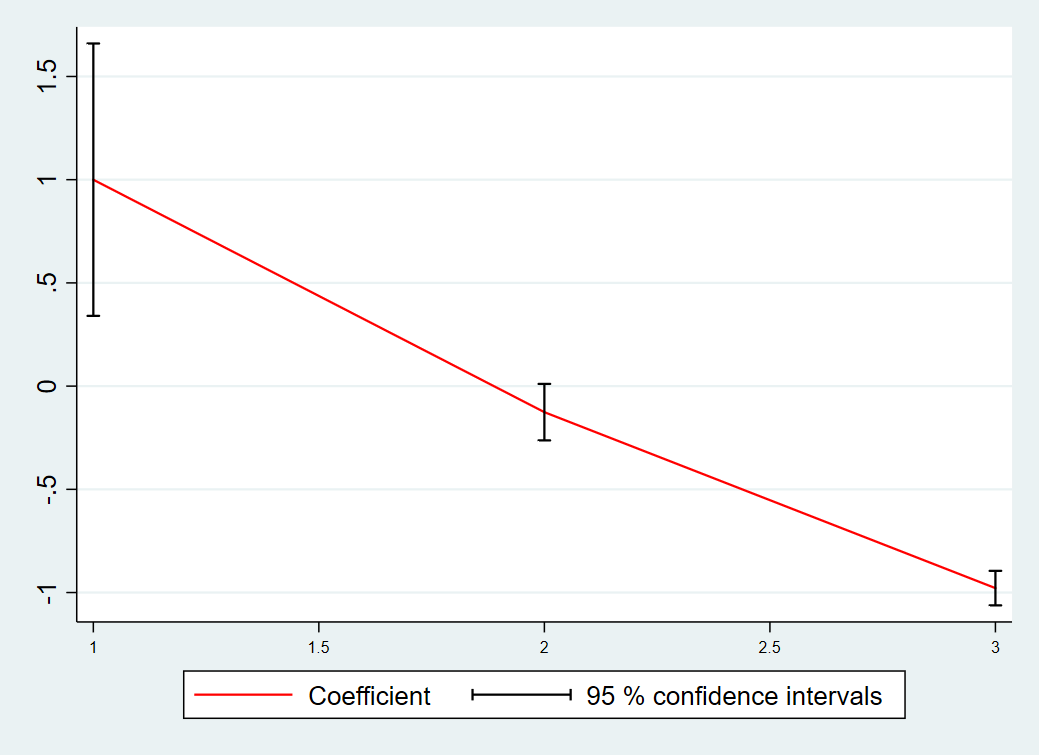
\includegraphics[width=\textwidth]{C:/Users/mariu/Documents/Master_Thesis/Master_thesis/Pics_graphs/IRF_no_controls_prev_cases.png}\\
\end{minipage}\hfill% 
\begin{minipage}[t]{0.5\linewidth}\vspace{0pt} 
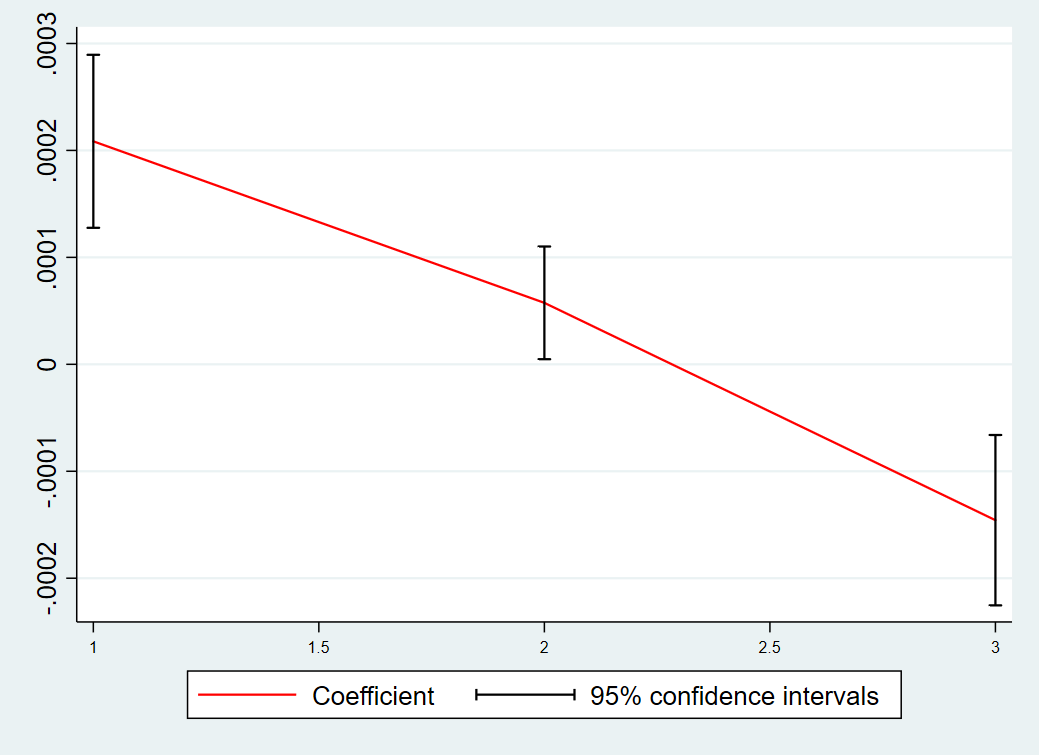
\includegraphics[width=\textwidth]{C:/Users/mariu/Documents/Master_Thesis/Master_thesis/Pics_graphs/IRF_no_controls_ebola_articles.png}\\
\end{minipage}\hfill% 
\caption{This figure shows the collection of local projections impulse response functions following \cite{jorda2005estimation} without including any control variables. The left half has the prevalence of Ebola cases as the measure for Ebola. On the right side, the measure for Ebola is the number of Ebola-related articles in the NYT. The maroon line marks the estimated coefficients while the shaded areas indicates the 95\% confidence intervals.}
\label{First Stage IRF - no controls}
\end{figure}

Unsurprisingly, both graphs draw a similar picture. The effect of the Ebola outbreak fades out with becoming economically close to zero already in 2015, the first year after the outbreak in the prevalence specification\footnote{Time $2$ in the graph}. The decreasing statistical significance in the same period supports the picture of a vanishing effect over time, with that effect being stronger in the case of prevalence specification. When using articles, the results suggests at in the first past the outbreak there might be some ongoing health-damaging effects since its coefficient is positive and statistically significant at the 95\% level. The unclarity regarding the follow-up year can be founded in intuition since there are several effects occuring simultaneously. First, the Ebola crisis is still impacting the countries heavily, even though at declining infection and fatality rates (CITATION NEEDED). At the same time, international efforts to contain the outbreak show signs of success (CITATION NEEDED). \\
In either specification, it becomes evident that in 2016 the impact is life-enhancing. Mortality rates in the treatment group drop significantly, in the economic and statistical sense. This result is very intuitive. In 2016, the WHO declared that all three countries can be considered Ebola-free (\cite{world2016latest}). Significant, positive results for continuing effects in 2016 would capture long-term effects for longer than 2 years. Altough not impossible, most long-term effects of Ebola confirmed by researchers last up to two years but hardly longer (\cite{clark2015long} and \cite{rowe1999clinical}). Contesting theories such that an increased mortality rate of weakend health workers leads to higher overall mortality rate since it lowers quality and quantity of the provided health care, as carefully outlined in \cite{evans2015next} does not appear to be a prevailing force in the direct aftermath. \\
The observed negative  on the other hand can be explained by two potential factors. Firstly, international investments in health infrastructure and increased development aid could lower post-Ebola mortality rates. There is some evidence suggesting that official development aid increases in the aftermath of a natural disaster, though small in size (\cite{becerra2014foreign}). \\
In contrast to this, there may simply be mean reversion as considered a potential problem in the context of health convergence investigated by \cite{jayachandran2009life}. \\
If it was the a reason in the same category as the earlier explanation rather than the latter explanation, we would expect to see a level shift in future health outcomes since it likely provides benefits beyond the mean. Mean reversion does not exhibit the same benefits. Future reasearch could exploit this pattern. Further, undetected in my impulse response function are any sorts of long-term effects that firstly occur in the years after the considered horizons. An example could be long-term effects in the setting of the fetal origins hypothesis (\cite{almond2011killing}). If in-utero malnutrition or stress trigger worse health and education outcomes, children of the effected mothers would still suffer consequences. \\
Adding control variables following the preferred specification of column (III) and (IV) of table \ref{Control results} only confirms the overall picture. As can be seen in figure \ref{First Stage IRF - with controls}, the trend approximately equals the trend in the previous graphs. If anything, we observe some difference in the behaviour of the second post-intervention estimations. The estimates lose some their statistical significance but are similar in economic magnitude. The post-intervention year $\tau + 1$ does not appear to bear any statistical significance anymore.

\begin{figure}[!ht]
\begin{minipage}[t]{0.5\linewidth}\vspace{0pt} 
\includegraphics[width=0.8\textwidth]{C:/Users/mariu/Documents/Master_Thesis/Master_thesis/Pics_graphs/IRF_controls_prev_cases.png}\\
\end{minipage}\hfill% 
\begin{minipage}[t]{0.5\linewidth}\vspace{0pt} 
\includegraphics[width=0.8\textwidth]{C:/Users/mariu/Documents/Master_Thesis/Master_thesis/Pics_graphs/IRF_controls_articles.png}\\
\end{minipage}\hfill% 
\caption{Figure \ref{First Stage IRF - with controls} is the collection of local projections impulse response functions following \cite{jorda2005estimation} with including the set of control variables as specified in column III and IV of table \ref{Control results}. The left half has the prevalence of Ebola cases as the measure for Ebola. On the right side, the measure for Ebola is the number of Ebola-related articles in the NYT. The maroon line marks the estimated coefficients while the shaded areas indicates the 95\% confidence intervals.}
\label{First Stage IRF - with controls}
\end{figure}

Before turning to the second stage results, there is need to examine the standard errors of the DiD. Subsection ??? does that.

\subsubsection{Biased Standard Errors}

In economics, clustered data is commonly used for empirical estimation. As already stated in work such as \cite{moulton1990illustration}, this can cause problematic consequences for inference if there is correlation within a cluster. As a result, many empirical studies use cluster robust variance estimator (CVRE).\\
In the DiD framework, there are three main problems arising when using CVRE. Primarily and widely discussed after the seminal work by \cite{bertrand2004much}, is the issue of few clusters. Secondly, \cite{conley2011inference} note that the standard errors will be severly biased if the DiD estimator lacks sufficient treated clusters. The last condition demands similar amount of datapoints for each cluster. \cite{carter2017asymptotic} and \cite{mackinnon2017wild} show theoretical and practical simulation on this condition. In the following paragraphs, I will expound the relevance of these concerns for my investigation. \\
The first condition can be rephrased as a requirement that the number of clusters goes to infinity in order to ensure consistency of the estimator. If this is condition is only marginally satisfied, the DiD tends to over-reject and t-statistics grow artificially large. The main mechanism at work is serial correlation in the error term. This is in large parts due to the intervention variable itself for it being a dummy variable (\cite{bertrand2004much} or \cite{donald2007inference}). Altough there is no clear rule of what "marginally satisfied" means, results by \cite{cameron2008bootstrap} suggest that 40 clusters are enough to suffice this condition, given a balanced panel. \\
The baseline regression results should not expose severely biased standard errors in this respect since the clsuter number of 40 seems highi enough. However, when dealing with the restults containing the control variables too this could prove an issue. With only 34 clusters, the model might suffer from over-rejection. There are several suggestions when dealing with this problem. For instance, a cluster-by-group approach  as proposed in \cite{bertrand2004much} or the wild cluster bootstrap following \cite{cameron2008bootstrap}. \\
According to \cite{conley2011inference} the same difficulty arises when the overall number of clusters is sufficiently large, but the number of treated units small. They show that the noise biasing the estimated fixed-effects regression yields consistent estimates only decreases with number of treated units but not with the overall number of clusters. While the former solution proposals are still valid, they propose a special form of randomization inference. While they do state a clear cut-off when the number of treated units is too small, they show that under some circumstances even as much as ten treated clusters are not sufficient to have unbiased standard errors with the standard procedure. Subsequently, having three treated clusters, as this study does, seems particularly vulnerable to this reasoning. \\
In the light of recent research most of these solution attempts have been shown to yield biased results themselves, at least in a practicioner's world. \cite{mackinnon2017wild} show that standard procedures such as \cite{bertrand2004much} or \cite{cameron2008bootstrap} fail when presented with unequally sized clusters or clusters are too few in numbers. They further prove that restricted wild cluster bootstrap underrejects for samples smaller than 4 but the unrestricted wild cluster bootstrap overrejects. They conclude that the true standard errors should fall within that interval. In a follow-up study, \cite{mackinnon2018wild} propose sub-clustering to narrow down the margin of the interval. \\
This is, as the previous point, relevant for this study. Since clustering is assumed to happen at the state level but trade is measured with country pairs each cluster has a different number of observations. For example, the Chad has an amount of 5899 country pair observations making up 4.63\% of the total sample. The South Sudan on the other hand, has a total of 1241 observations with accumulates to 0.97 \% (both, however, are part of the control group). That means, the size of the Chad is almost five times the size of South Sudan's. On average, treated cluster in this study incorporate 3042 observations in contrast to 3358 for the untreated. The ratio of treated to untreated is 1.1 which should introduce, if any, a small amplifying bias on wildly bootstrapped standard errors. \\
Out of the three potential causes for biased standard errors, at least one - few treated clusters - is highly likely to affect the estimated results. While the procedure by \cite{conley2011inference} sufficies for few treated clusters, it fails if the slightly unequal cluster sizes turn out to be relevant. Therefore, I stick to the procedure suggested by \cite{cameron2008bootstrap} and improved by \cite{mackinnon2018wild} which can account for this.
But before turning to the results, I believe the terms of unrestricted and restricted cluster bootstrap deserve some explanation. \\
Generally, the bootstrap is a resampling method to evaluate the likelihood of reaching the same result as in the original estimation with a subset of data. In more detail, the researcher draws, with replacement, a set of random number from the originial dataset until she reaches the desired number of \textit{G} bootstrap samples. Next, one has to regress for each bootstrap sample and find the corresponding t-statistic. Lastly, the original estimation can be evaluated against the distribution of bootstrapped results. While cluster bootstrapping, as described in this paragraph, is a powerful tool \cite{mackinnon2017wild} show that in the presences of few treated clusters it yields misleading results. That is because with very few treatment observations many bootstrap samples will have zero for every treatment observation.\\
Wild cluster bootstrap is similar to this but solves this problem. Hereby, the original regression is calculated, yielding the standard cluster-robust t-statistic $ t_j $ for $\beta_j = 0$. In \cite{cameron2008bootstrap}, the restricted wild cluster approach, the next step is to regress again given that $\beta_j = 0$. This gives the new estimates $\tilde{\beta}$ and $\tilde{u}$. Now, for each bootstrap sample one regresses
\begin{align}
\textbf{y}^{b} = \textbf{X} \tilde{\beta} + \textbf{\textit{v}} \tilde{\textbf{u}}
\end{align}

where $\textbf{\textit{v}}$ represents an augmented weight vector with the length of the number of clusters. The weights are drawn from a Rademacher distribution. We obtain the estimates $\hat{\beta}^{b}$ and $\hat{\textbf{u}}^{b}$. For each bootstrap sample the t-statistic $t_j^{b} $ for the hypothesis $\hat{\beta}^{b} = \tilde{\beta}$ can be computed. Lastly, \cite{cameron2008bootstrap} recommend calculating new p-values to by comparing the original t-statistic to the distribution of $t_j^{b} $. \\
\cite{mackinnon2017wild} explain that the unrestricted wild cluster bootstraps is essentially equal to the above procedure with the only difference being that $\tilde{\beta}$ is simply being the set to equal $\hat{\beta}$. $\hat{\beta}$ is the originally estimated coefficient.\\
And yet, with very few treated clusters even a wild bootstrap can fail. In short, if the original error term produces large t-statistics, the Rademacher weights with its bimodal properties will create even bigger bootstrap t-statistcs. \footnote{see \cite{mackinnon2017wild} for the full proof} As a rule of thumb, they suggest that studies with fewer than four treated clusters will show misleading wild cluster bootstrap standard errors. \\
To solve this, \cite{mackinnon2018wild} suggest to use sub-cluster to reduce the proportions of the error. \cite{djogbenou2018asymptotic} ground the wild bootstrap theoretically when discovering that the results of sub-clustering is asymptotically valid even when there is intra-cluster correlation. Thereby, I follow the implementation as in \cite{roodman2019fast} by using their Stata package \textbf{bootstrap}.\\
Every estimation employs 1499 bootstrap replication and is based on the baseline estimation as in Table \ref{Baseline results}. Table \ref{Wild cluster bootstrap} and \ref{Wild cluster bootstrap with controls} report the confidence intervals at the 95\% of significance. Table \ref{Wild cluster bootstrap} does not include any control variables. \\
Table \ref{Wild cluster bootstrap} confirms most of the findings explored earlier. Firstly, we do observe major changes across different wild cluster bootstraps and cluster specification. For instance in column (II) where we observe the expected behaviour. On the one side, the hypothesis of no effects of the Ebola variable on health outcomes can not be rejected at any common level of significance, however by a close margin. On the other side, the unrestricted wild cluster bootstrap shows, basically, the same confidence intervals and p-value as the original estimation. When using sub-clusters the values converge strongly. Now, both estimates are significant on the 1\% level and show very similar confidence intervals to each other but also to the original estimates. \\
Column I is behaving differently. Unexpectedly, the restricted wild cluster bootstrap exhibits a long left-side tail for the confidence interval such that the estimated sign now turns negative. \\
?? WHY ??? \\
When clustering the bootstrap results on a country-pair level, the restricted bootstrap takes on the expected form and converges to the unrestricted bootstrap. The level of significance can now be of the estimate around the 10\% level.

\begin{table}[htbp] \centering
\caption{Wild cluster bootstrap \label{Wild cluster bootstrap}}
\resizebox{\textwidth}{!}{
\begin{tabular}{lcccc} \hline
 & \multicolumn{2}{c}{(I)} & \multicolumn{2}{c}{(II)}  \\ \vspace{3pt}
Treatment group & \multicolumn{2}{c}{Three countries} & \multicolumn{2}{c}{Three countries}  \\ \vspace{3pt}
Treatment variable & \multicolumn{2}{c}{Case prevalence} & \multicolumn{2}{c}{Ebola articles} \\ \vspace{3pt}
Estimate & \multicolumn{2}{c}{0.9716} & \multicolumn{2}{c}{0.02} \\ \vspace{3pt}
Cluster robust s.e. & \multicolumn{2}{c}{0.3169} & \multicolumn{2}{c}{0.004} \\ \vspace{3pt}
t-statistic & \multicolumn{2}{c}{3.07} & \multicolumn{2}{c}{5.21} \\ \hline \vspace{3pt}
\vspace{3pt} P-values \& CI & P value & CI & P value & CI \\ \vspace{3pt}
Initial results & 0.004  & [0.331, 1.613] & 0.000  & [0.012, 0.028]\\ \vspace{3pt}
Bootstrap by country, restricted & 0.105 & [-631.6, 24.2] & 0.1054 &  [-.1698, .2974] \\ \vspace{3pt}
Bootstrap by country, unrestricted & 0.28& [-.461, 2.404] & 0.0000 & [.01224, .02828]  \\ \vspace{3pt}
Bootstrap by country-pair, restricted & 0.0856 & [-1.649, 5.502] & 0.009 & [.009949, .03193] \\ \vspace{3pt}
Bootstrap by country-pair, unrestricted & 0.1381 & [-.5862, 2.529] & 0.000 & [0.012, 0.028] \\ \hline \vspace{3pt}
\end{tabular}
}
\end{table}

The results for the article measurement of Ebola appear to confirm the initial results strengthening the confidence in these. The results for the case prevalence rate are not as convincing but nevertheless point into the same direction. \\
The missing step now is to find out if the results with control variables offer the same robustness. As already shown earlier, the estimation including control variable has moderately fewer clusters. In fact, there are 6 fewer control clusters now. Theoretically, this should amplify errors in both bootstrap methods. We would therefore expect higher p-values (restricted) and lower p-values (unrestricted) than in Table \ref{Wild cluster bootstrap}, although it might not be of relevant magnitude. \\
\ref{Wild cluster bootstrap with controls} shows the predicted behaviour. The restricted bootstrap underrejects while the unrestricted bootstrap overrejects. Column (I) shows the restricted bootstrap indicating statistically insignificant results while the unrestricted claims both to be statistically significant on the 1\% level. Sub-clusters tend to the same coonvergence as in Table \ref{Wild cluster bootstrap}. Especially the restricted wild cluster bootstrap converges towards statistical significance. The unrestricted estimate remains very constant and is still highly significant. Here as above, the article estimation seem to be very robust and unaffected by the few treated clusters.\\

\begin{table}[htbp] \centering
\caption{Wild cluster bootstrap with controls \label{Wild cluster bootstrap with controls}}
\resizebox{\textwidth}{!}{
\begin{tabular}{lcccc} \hline
 & \multicolumn{2}{c}{(I)} & \multicolumn{2}{c}{(II)}  \\ \vspace{3pt}
Treatment group & \multicolumn{2}{c}{Three countries} & \multicolumn{2}{c}{Three countries}  \\ \vspace{3pt}
Treatment variable & \multicolumn{2}{c}{Case prevalence} & \multicolumn{2}{c}{Ebola articles} \\ \vspace{3pt}
Estimate & \multicolumn{2}{c}{1.15} & \multicolumn{2}{c}{0.015} \\ \vspace{3pt}
Cluster robust s.e. & \multicolumn{2}{c}{0.301} & \multicolumn{2}{c}{0.005} \\ \vspace{3pt}
t-statistic & \multicolumn{2}{c}{3.82} & \multicolumn{2}{c}{2.98} \\ \hline \vspace{3pt}
\vspace{3pt} P-values \& CI & P value & CI & P value & CI \\ \vspace{3pt}
Initial results & 0.001 & [0.537, 1.763] & 0.005 &  [0.005, 0.025]\\ \vspace{3pt}
Bootstrap by country, restricted & 0.165 & [-23.98, 16.41] & 0.121 &  [-0.073, 0.089]  \\ \vspace{3pt}
Bootstrap by country, unrestricted & 0.001 & [0.538, 1.761] & 0.003  & [0.005, 0.024]  \\ \vspace{3pt}
Bootstrap by country-pair, restricted & 0.148 & [-1.619, 4.399] & 0.065 & [-0.003, 0.029]\\ \vspace{3pt}
Bootstrap by country-pair, unrestricted & 0.003 & [0.442, 1.857] & 0.003 & [0.005, 0.024] \\ \hline \vspace{3pt}
\end{tabular}
}
\end{table}

Overall, the bootstrap results seem to confirm the results of the cluster-robust variance matrix estimator. Therefore, we can now turn towards the second stage of the estimation.

\subsection{Second Stage}

After having established, a valid difference-in-difference set-up and relevance for the coefficient of interest beyond a reasonable scepticism, we can see how the estimated health coefficients influence trade outcomes. Namely, I will focus on exports, imports as well as trade balance.\\
According to the theoretical simulation drawn out in section ???, we have clear expectations about the coefficient signs and an indication about economic as well as statistical relevance. For exports, we expect a negative sign and likely statistical significance. The same pattern is supposed to hold for the trade balance. Imports should follow a different pattern. While a negative sign on impact is expected, this should turn positive in the second post-shock period. In the first year after the shock, we expect still a negative sign but a smaller coefficient. Since the real data only cover the first three periods of the shock, we expect a negative sign. Studies including a larger time horizon are expected to find a positive sign for a contemporaneous regression. Given the generally smaller deviation from zero in the simulation, the effect might be undistinguishable from zero. Therefore, doubt about statistical significance are reasonable.

\subsubsection{Baseline}

I start to draw out the second stage by presenting the regression equation following an instrumental variable design.
\begin{align}
Y_{ijt} =  \beta \mathbf{H_{it}} +  X_{it}'\eta + \alpha_{ij} + \zeta_t + \epsilon_{it}
\end{align}
with 
\begin{align}
\mathbf{H_{it}} =  \beta Z_{it} +  Q_{it}'\nu + X_{it}'\eta + \pi_{it} + \alpha_i + \zeta_t + \epsilon_{it}
\end{align}
being equal to equation (22) of the previous section. $i$ indexes the country of origin and $j$ the corresponding trading partner. To fix ideas, $i$ can be any of the 40 countries of control or treatment group while $j$ is any country trading with $i$. $t$ indexes years. $Q_{it}'\nu$ represents the control variables of the first stage while $X_{it}'\eta$  represents those of the second stage. As in the previous regression, $\pi_{it}$ represents a country-pair-specific linear trend across time. $\alpha_{ij}$ accounts for country-pair specific fixed effects with $\zeta_t$ controlling for time fixed effects. \\
An intuitive second stage result without any control variables, can be found in Table \ref{Second Stage Baseline}. While the first two columns use exports as the dependent variable, the middle columns use imports. The two columns on the right regress on the trade balance. All three variable are measured in constant 2010 Dollars. A natural logarithmic transformation to exports and imports has been applied in order to ease interpretation.

\begin{table}[htbp] \centering
\caption{Second Stage Baseline \label{Second Stage Baseline}}
\resizebox{\textwidth}{!}{
\begin{tabular}{lcccccc} \hline
 & (1) & (2) & (3) & (4) & (5) & (6) \\
Dependent Variable & \multicolumn{2}{c}{Exports} & \multicolumn{2}{c}{Imports}  & \multicolumn{2}{c}{Trade Balance}  \\ \hline
\vspace{4pt} & \begin{footnotesize}\end{footnotesize} & \begin{footnotesize}\end{footnotesize} & \begin{footnotesize}\end{footnotesize} & \begin{footnotesize}\end{footnotesize} & \begin{footnotesize}\end{footnotesize} & \begin{footnotesize}\end{footnotesize} \\
Log Mortality Rate & -3.203*** & -3.179*** & 0.0591 & 0.0649 & 11.37 & 11.28 \\
 & \begin{footnotesize}(0.677)\end{footnotesize} & \begin{footnotesize}(0.675)\end{footnotesize} & \begin{footnotesize}(0.0499)\end{footnotesize} & \begin{footnotesize}(0.0494)\end{footnotesize} & \begin{footnotesize}(28.53)\end{footnotesize} & \begin{footnotesize}(28.68)\end{footnotesize} \\
\vspace{4pt} & \begin{footnotesize}\end{footnotesize} & \begin{footnotesize}\end{footnotesize} & \begin{footnotesize}\end{footnotesize} & \begin{footnotesize}\end{footnotesize} & \begin{footnotesize}\end{footnotesize} & \begin{footnotesize}\end{footnotesize} \\
Instrument & Prevalence & Articles & Prevalence & Articles & Prevalence & Articles \\
\vspace{4pt} & \begin{footnotesize}\end{footnotesize} & \begin{footnotesize}\end{footnotesize} & \begin{footnotesize}\end{footnotesize} & \begin{footnotesize}\end{footnotesize} & \begin{footnotesize}\end{footnotesize} & \begin{footnotesize}\end{footnotesize} \\
Observations & 57,794 & 57,794 & 64,203 & 64,203 & 84,288 & 84,288 \\
Country-pairs & 6,365 & 6,365 & 6,076 & 6,076 & 7,232 & 7,232 \\
Two-way FE & Yes & Yes & Yes & Yes & Yes & Yes \\
F-statistic first stage & 34.64 & 47.49 & 41.77 & 58.36 & 39.81 & 52.08 \\
No. of clusters & 40 & 40 & 40 & 40 & 40 & 40 \\
Cluster & &\multicolumn{2}{c}{Country pair} \\ \hline
\multicolumn{7}{c}{\begin{footnotesize} Clustered standard errors in parentheses. \end{footnotesize} }\\
\multicolumn{7}{c}{\begin{footnotesize} *** p$<$0.01, ** p$<$0.05, * p$<$0.1\end{footnotesize}} \\\end{tabular}
}
\end{table}

When taking a look at exports, we find strong economic and statistical relevance of health as a determinant. We associate an increase in the mortality rate by one percent with an decrease in exports by about three percent. This is independent of the instrument used. Having three treated clusters is subject to them same concern voice in section ?????. The unrestricted as well as the restricted wild clustered bootstrap errors show highly significant results with 95\% confidence intervals between approximately -4.3 and -1.9 for both cases. That leaves us with good confidence in the economic and statistical relevance of health in determining exports.\footnote{More results can be obtained from the author}\\
When we turn to imports, we find the unexpected, posititve sign.  Economically, an increase in mortality rates by one percent would be expected to yield an increase in imports by about 0.06\%. A t-statistic of about 1 in both specifications confirms our initial concerns regarding the relevance of health outcomes for import behaviour. \\
With respect to incomes, the simple model prognosted a reduction in income due to the overall loss in output allowing less consumption and investment with in return implies less imports. These mechanism does not seem to be dominant. \\
Agnostically surprising, the trade balance does not follow the trend of exports at all. On the contrary, the estimated sign is positive and the esimation fails reject to null of no statistical significance. The effect seems to be similar to the effect on imports, instead. The most intuitive answer to this would be that imports are greater in value terms than exports. The theoretical simulation is an exchange economy in contrast to the real economy where real prices matter. And indeed, the data exhibits an inequality as can be seen in Figure \ref{Export-Imports Scatter}.

\begin{figure}[!ht]
\begin{center}\caption{Export-Imports Scatter \label{Export-Imports Scatter}}
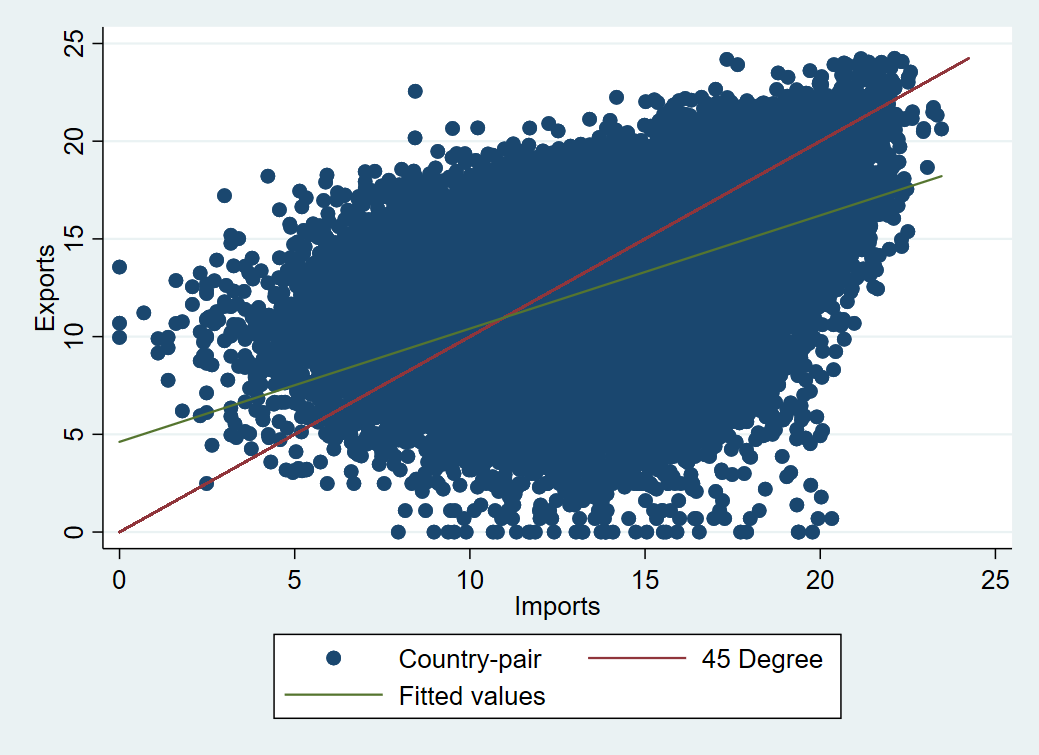
\includegraphics[width=0.8\textwidth]{C:/Users/mariu/Documents/Master_Thesis/Master_thesis/Pics_graphs/Exports_imports_scatter.png}\\
\end{center}
\end{figure}

Here, every blue dot represents a country-pair's value of exports and imports. The red line marks the 45 degree. If imports and exports were equal we would expect the cloud to be symmetric above and below the red line. However, the part below the red line seems swollen indicating imports being larger than exports for the employed sample. The green line shows a more thorough approach to answer the same question. It is a simple regression of imports on exports. Since the slope of the green line is smaller than of the red line, we can conclude that exports are less in size than imports for our sample. 
Another potential reason are prices. In the simple set-up above, \\

\subsubsection{Exclusion Restricition}
The validity of any instrumental variable approach depends crucially on the exclusion restriction and relevance assumption to hold. Relevance can be easily tested. In any of the above specification and any of the following specification, we observe f-statistics considerably larger than 10. A value of 10 is commonly deemend suffiencient to avoid a weak instrument (\cite{stock2002testing}). \\
The exclusion restriction is not easily testable and needs careful discussion. The essence of the restriction is that the instrument only works through the instrument and nothing else. Here, that any consequences of the Ebola Virus Disease only work via mortality rates.\\
There are some concerns regarding this. Firstly, one could imagine a scenario where Ebola does not cause fatalities but still forces people to stop working or shift their consumption behaviour. Another concern is trust. If the mere knowledge of being exposed to Ebold before having experienced any outbreak the exclusion restriction likely is violated. A consciousness of the diseases in combination with enough economic and cultural flexibility allows consumers to change their consumption bundle accordingly just by evaluating the risk factors ona regular basis. In the same way firms could adjust their capital investment strategies to prevent a shock to productivity to affect them.\\
The first concern is rebuttable. As already outlined, EVD is a highly fatal disease with fatality rates ranging between 41 and 89\% (\cite{chowell2014transmission}). In addition, the authors outline that these estimates are likely to be the lower ends due to a sampling bias. Not everyone experiencing the symptoms might have reported them due to, for instance, a lack of awareness. Higher mortality rates caused only indirectly by weakening the immune system and subsequently increasing fatality rates of other diseases are also not included. This has been shown for some other fatal diseases such as Tuberculosis (\cite{parpia2016effects}).\\
The other concern is harder to refute. To fix thoughts, assume there is a single case of EVD and quarantined immediately. Assume further, that there is general, perfect information about EVD and about the case. This would in all likelihood not change the mortality rate of the country, in the best circumstances not even of any individual. If there is high trust in medical institutions and government's ability to deal with these sort of situations, consumers and firms would not change their economic choices. However, if the occurence of such a case reduces trust actors are prone to change their behaviour. In short, if trust is affected by a limited outbreak it could change economic decisions without seeing any change in mortality rates. In a permanent setting, agents would adjust their behaviour according to risk factors that usually don't affect choices. Meteorological factors can be stated as such (\cite{alexander2015factors}). The exclusion restriction would be violated. \\
However, there are some indicators pointing towards incompleteness of the premisses to match the above chain of reasoning. \cite{gonzalez2017epidemics} finds, trust is affected more with increased severity of the EVD. If the pattern is truly like described above, we would expect to see an equally dramatic shift independent of the intensity. Instead, it appears that trust is only affected after a fatal outbreak indicating that the exclusion restriction holds. Further, the assumption of perfect information is questionable. As I argued in section ????, EVD hit experts, health officials and consumers by surprise. Without knowing about the possibility of an outbreak it is hard to argue that agents changed their choices independent of the outbreak.\\
All in all, the exclusion restriction seems to hold.

\subsubsection{Control variables}

As already suggested by the semi-structural equation derived in section ???, control variables should be taken into account. Before including the variables as proposed by that equation, I consider only to include output. Since, as derived in section ???, the effect should work via production, we would expect any health effects on trade to diminish economically and statistically once output itself is included. \\ 

\begin{table}[htbp] \centering
\caption{Second Stage Output \label{Second Stage Output}}
\resizebox{\textwidth}{!}{
\begin{tabular}{lcccc} \hline
 & (1) & (2) & (3) & (4) \\
Dependent Variable & Exports & Imports & Trade Balance & GDP \\ \hline
\vspace{4pt} & \begin{footnotesize}\end{footnotesize} & \begin{footnotesize}\end{footnotesize} & \begin{footnotesize}\end{footnotesize} & \begin{footnotesize}\end{footnotesize} \\
Log Adult Mortality Rate & -2.443** & 0.00545 & 47.64** & -0.893*** \\
\vspace{4pt} & \begin{footnotesize}(1.210)\end{footnotesize} & \begin{footnotesize}(0.0675)\end{footnotesize} & \begin{footnotesize}(22.70)\end{footnotesize} & \begin{footnotesize}(0.140)\end{footnotesize} \\
Log GDP p.c. & 0.849 & -0.0541 & 37.61 &  \\
 & \begin{footnotesize}(0.836)\end{footnotesize} & \begin{footnotesize}(0.0650)\end{footnotesize} & \begin{footnotesize}(44.07)\end{footnotesize} & \begin{footnotesize}\end{footnotesize} \\
\vspace{4pt} & \begin{footnotesize}\end{footnotesize} & \begin{footnotesize}\end{footnotesize} & \begin{footnotesize}\end{footnotesize} & \begin{footnotesize}\end{footnotesize} \\
Instrument & Prevalence & Prevalence & Prevalence & Prevalence \\
\vspace{4pt} & \begin{footnotesize}\end{footnotesize} & \begin{footnotesize}\end{footnotesize} & \begin{footnotesize}\end{footnotesize} & \begin{footnotesize}\end{footnotesize} \\
Observations & 56,188 & 62,350 & 81,872 & 119,421 \\
Number of country-pairs & 6,184 & 5,893 & 7,022 & 7,085 \\
Two-way FE & Yes & Yes & Yes & Yes \\
F-statistic first stage & 493.4 & 493.4 & 493.4 & 493.4 \\
No. of clusters & 38 & 38 & 38 & 38 \\ 
Cluster & \multicolumn{2}{c}{Country pair} \\ \hline
\multicolumn{5}{c}{\begin{footnotesize} Clustered standard errors in parentheses\end{footnotesize}} \\
\multicolumn{5}{c}{\begin{footnotesize} *** p$<$0.01, ** p$<$0.05, * p$<$0.1\end{footnotesize}} \\
\end{tabular}
}
\end{table}
Table \ref{Second Stage Output} shows these predictions are only partially correct. Indeed, coefficients as well as t-statistics are closer to zero in comparison to Table \ref{Second Stage Baseline}. That indicates that a significant share of the overall works via the production. For exports, the estimated share of production of the overall effect is approximately 24\%. With regards to imports, 90\% of the estimated coefficient in Table \ref{Second Stage Baseline} are dropped. Given that the original estimate was already statistically not significant, a cautious interpretation is needed. Albeit, it poses a intruiging argument for the relevance of production on importing behaviour. \\
Yet, about three quarters of the effect on exports is uncovered by either model mechanism proposed in the theoretical part. The implication is that both models, simple and expanded, are lacking important features that explain health impacts on export patterns. This poses an interesting question for future research. Including direct quaratines or investment restriction in a general fashion might be interesting for such. \\
Further interesting is the fact that we associate any increase in mortality with an increase in the trade balance despite reduced exports and seemingly unimpacted imports. Since all terms are measured in 2010 dollar, any price adjustment should be accounted for. \\
However, in more detail, we modelled the precise channel of any health shock via labour supply and productivity. Therefore, it makes sense to split output into it's parts and see whether both parts are relevant. In Table \ref{Second Stage Control Variables}, I included capital, population and tariffs. Capital and Labour are main production inputs. So if there is no reduction by including these two control variables we would expect productivity to be the main driver. Further, tariffs are included to correct for the most obvious obstacles to trade that have been omitted in the models but might have an influence in the data.

\begin{table}[htbp] \centering
\caption{Second Stage Control Variables \label{Second Stage Control Variables}}
\resizebox{\textwidth}{!}{
\begin{tabular}{lcccccc} \hline
 & (1) & (2) & (3) & (4) & (5) & (6) \\
Dependent Variable & \multicolumn{2}{c}{Exports} & \multicolumn{2}{c}{Imports}  & \multicolumn{2}{c}{Trade Balance}  \\ \hline
\vspace{4pt} & \begin{footnotesize}\end{footnotesize} & \begin{footnotesize}\end{footnotesize} & \begin{footnotesize}\end{footnotesize} & \begin{footnotesize}\end{footnotesize} & \begin{footnotesize}\end{footnotesize} & \begin{footnotesize}\end{footnotesize} \\
Log Adult Mortality Rate & -3.205*** & -3.205*** & 0.274 & 0.274 & 56.21 & 56.21 \\
\vspace{4pt} & \begin{footnotesize}(0.886)\end{footnotesize} & \begin{footnotesize}(0.886)\end{footnotesize} & \begin{footnotesize}(0.240)\end{footnotesize} & \begin{footnotesize}(0.240)\end{footnotesize} & \begin{footnotesize}(55.85)\end{footnotesize} & \begin{footnotesize}(55.85)\end{footnotesize} \\
Log Population & -0.511 & -0.511 & 0.0692 & 0.0692 & -2.092 & -2.092 \\
\vspace{4pt} & \begin{footnotesize}(0.442)\end{footnotesize} & \begin{footnotesize}(0.442)\end{footnotesize} & \begin{footnotesize}(0.160)\end{footnotesize} & \begin{footnotesize}(0.160)\end{footnotesize} & \begin{footnotesize}(64.10)\end{footnotesize} & \begin{footnotesize}(64.10)\end{footnotesize} \\
Log Capital (t-1) & 0.277* & 0.277* & 0.0312 & 0.0312 & 6.842 & 6.842 \\
\vspace{4pt} & \begin{footnotesize}(0.160)\end{footnotesize} & \begin{footnotesize}(0.160)\end{footnotesize} & \begin{footnotesize}(0.0400)\end{footnotesize} & \begin{footnotesize}(0.0400)\end{footnotesize} & \begin{footnotesize}(9.471)\end{footnotesize} & \begin{footnotesize}(9.471)\end{footnotesize} \\
Tariff size (\%) & 0.0225 & 0.0225 & -0.000835 & -0.000835 & -4.494 & -4.494 \\
 & \begin{footnotesize}(0.0235)\end{footnotesize} & \begin{footnotesize}(0.0235)\end{footnotesize} & \begin{footnotesize}(0.00212)\end{footnotesize} & \begin{footnotesize}(0.00212)\end{footnotesize} & \begin{footnotesize}(2.939)\end{footnotesize} & \begin{footnotesize}(2.939)\end{footnotesize} \\
\vspace{4pt} & \begin{footnotesize}\end{footnotesize} & \begin{footnotesize}\end{footnotesize} & \begin{footnotesize}\end{footnotesize} & \begin{footnotesize}\end{footnotesize} & \begin{footnotesize}\end{footnotesize} & \begin{footnotesize}\end{footnotesize} \\ 
\vspace{4pt} Instrument & Prevalence & Articles & Prevalence & Articles & Prevalence & Articles \\ 
\vspace{4pt} & \begin{footnotesize}\end{footnotesize} & \begin{footnotesize}\end{footnotesize} & \begin{footnotesize}\end{footnotesize} & \begin{footnotesize}\end{footnotesize} \\ 
Observations & 34,146 & 34,146 & 37,318 & 37,318 & 49,332 & 49,332 \\
Number of country-pairs & 5,168 & 5,168 & 5,062 & 5,062 & 6,136 & 6,136 \\
Two-way FE & Yes & Yes & Yes & Yes & Yes & Yes \\
F-statistic first stage & 5455 & 5455 & 4708 & 4708 & 4155 & 4155 \\
No. clusters & 35 & 35 & 35 & 35 & 35 & 35 \\ 
Cluster & &\multicolumn{2}{c}{Country pair} \\ \hline
\multicolumn{7}{c}{\begin{footnotesize} Clustered standard errors in parentheses\end{footnotesize}} \\
\multicolumn{7}{c}{\begin{footnotesize} *** p$<$0.01, ** p$<$0.05, * p$<$0.1\end{footnotesize}} \\
\end{tabular}
}
\end{table}
It becomes evident by looking at Table \ref{Second Stage Control Variables} that population, regardless of dependent variable and instrument, does not appear to be the main driver. Rather, we are hinted towards productivity as the prevalent force for the effects inside the productivity function.\\
Next, I consider a different specification of control variables. Hereby, the preferred regression design in Table \ref{Control results} is combined with the theoretical controls from Table \ref{Second Stage Control Variables}. The combination is shown in Table \ref{Second Stage Control Variables II}. It is important to state that I report only the results for the case prevalence as instrument since results differ on the thrid to fourth digit only.\footnote{The other results can be shared upon request.}

\begin{table}[htbp] \centering
\caption{Second Stage Control Variables II \label{Second Stage Control Variables II}}
\resizebox{\textwidth}{!}{
\begin{tabular}{lccc} \hline
 & (1) & (2) & (3) \\
Dependent Variable & Exports & Imports & Trade Balance \\ \hline
\vspace{4pt} & \begin{footnotesize}\end{footnotesize} & \begin{footnotesize}\end{footnotesize} & \begin{footnotesize}\end{footnotesize} \\
Log Adult Mortality Rate & -1.887* & -0.0075 & 85.53 \\
\vspace{4pt} & \begin{footnotesize}(1.078)\end{footnotesize} & \begin{footnotesize}(0.185)\end{footnotesize} & \begin{footnotesize}(63.04)\end{footnotesize} \\
Log Population & -0.224 & 0.307 & -125.1 \\
\vspace{4pt} & \begin{footnotesize}(1.464)\end{footnotesize} & \begin{footnotesize}(0.326)\end{footnotesize} & \begin{footnotesize}(127.2)\end{footnotesize} \\
Log Capital (t-1) & 0.246 & -0.0327 & -4.300 \\
\vspace{4pt} & \begin{footnotesize}(0.180)\end{footnotesize} & \begin{footnotesize}(0.0481)\end{footnotesize} & \begin{footnotesize}(11.66)\end{footnotesize} \\
Tariff size (\%) & -0.0014 & -0.0029 & -4.057** \\
\vspace{4pt} & \begin{footnotesize}(0.013)\end{footnotesize} & \begin{footnotesize}(0.0022)\end{footnotesize} & \begin{footnotesize}(1.885)\end{footnotesize} \\
Log GDP p.c. & 0.0008 & 0.131 & 178.7*** \\
\vspace{4pt} & \begin{footnotesize}(0.597)\end{footnotesize} & \begin{footnotesize}(0.139)\end{footnotesize} & \begin{footnotesize}(63.24)\end{footnotesize} \\
GDP Growth & 0.0083 & -0.0011 & -1.309*** \\
\vspace{4pt} & \begin{footnotesize}(0.0068)\end{footnotesize} & \begin{footnotesize}(0.0023)\end{footnotesize} & \begin{footnotesize}(0.452)\end{footnotesize} \\
Log Fatalities & -0.0123 & 0.0085 & -0.362 \\
\vspace{4pt} & \begin{footnotesize}(0.0218)\end{footnotesize} & \begin{footnotesize}(0.0066)\end{footnotesize} & \begin{footnotesize}(1.468)\end{footnotesize} \\
Internet Access (\% of pop) & -0.0352** & -0.0027 & -2.491* \\
\vspace{4pt} & \begin{footnotesize}(0.0165)\end{footnotesize} & \begin{footnotesize}(0.0038)\end{footnotesize} & \begin{footnotesize}(1.328)\end{footnotesize} \\
Living Urban (\% of pop) & 0.119*** & -0.0170 & 7.868 \\
 & \begin{footnotesize}(0.0381)\end{footnotesize} & \begin{footnotesize}(0.0106)\end{footnotesize} & \begin{footnotesize}(5.630)\end{footnotesize} \\
\vspace{4pt} & \begin{footnotesize}\end{footnotesize} & \begin{footnotesize}\end{footnotesize} & \begin{footnotesize}\end{footnotesize} \\
Instrument & Prevalence & Prevalence & Prevalence \\
\vspace{4pt} & \begin{footnotesize}\end{footnotesize} & \begin{footnotesize}\end{footnotesize} & \begin{footnotesize}\end{footnotesize} \\
Observations & 24,944 & 27,333 & 35,763 \\
Number of country-pairs & 4,446 & 4,395 & 5,318 \\
Two-way FE & Yes & Yes & Yes \\
F-statistic first stage & 13.28 & 13.28 & 13.28 \\
No. clusters & 36 & 36 & 36 \\ 
Cluster & \multicolumn{1}{c}{Country pair} \\ \hline
\multicolumn{4}{c}{\begin{footnotesize} Clustered standard errors in parentheses\end{footnotesize}} \\
\multicolumn{4}{c}{\begin{footnotesize} *** p$<$0.01, ** p$<$0.05, * p$<$0.1\end{footnotesize}} \\
\end{tabular}
}
\end{table}
We observe that, even after controlling for any theoretical impact and some other, relevant empirical factors, the results still suggests an statistical and economic relevant impact of health on exports. The economic margin is now roughly half the size of the initial estimates and the statistical relevance is estimated at the 10\% level.\\
Imports do not change considerably compared to Table \ref{Second Stage Output} hinting towards the importance of output in the change of imports. \\
The trade balance remains about where it was before in terms of statistical significance while the coefficient increased slightly.\\
Lastly, I ran regression to see for robustness with respect to different control group specifications. Results do not change when excluding countries that are neighbours or have had at least one incident. \\
Other research suggests, that even the results estimated here might be underestimating the true impact. \cite{thomas2015economic} find small impacts for officially unimpacted, sub-saharan countries. Therefore our results tend to underestimate the difference between treatment and control.

\subsubsection{Impulse response function}

The last step is to compare the impulse response functions (IRF) estimated empirically to the theoretical. Figure \ref{Second Stage IRF - no controls} shows the IRF of exports and imports the baseline estimation as reported in Table \ref{Second Stage Baseline}. We observe that the on-impact-drop in exports is followed by a convergence towards the pre-shock level of exports, as the left part of Figure \ref{Second Stage IRF - controls} demonstrates. The steeper slope of the empirical IRF suggests that the applied parameters of sluggishness are too strong. \\
The comparison is different for imports, as can be seen on the right side of the same graph. While the impact is not negative - in opposite to the theoretical simulation - it turns positive and statistically significant. This pattern is similar to the simple simulation but not observed in price-adjusted value. \\
The trade balance should, in theory, increase and later go below zero, according to the expanded model. Instead, we observe a real movement in the estimated coefficients around the value of zero. Overall, neither simple nor expanded model seems to predict the unaffectedness of the trade balance as demonstrated in Figure \ref{IRF - Trade Balance} on the left side.

\begin{figure}[!ht] 
\begin{minipage}[t]{0.5\linewidth}\vspace{0pt} 
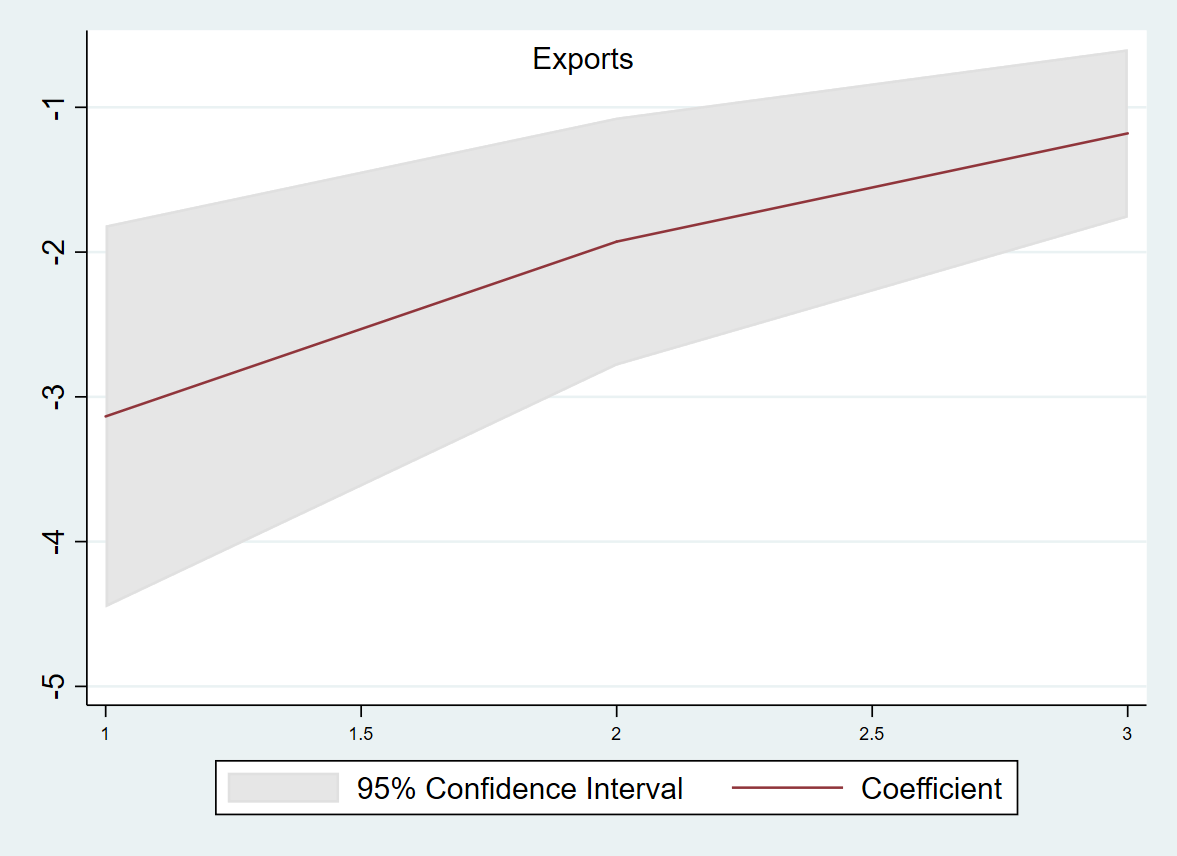
\includegraphics[width=\textwidth]{C:/Users/mariu/Documents/Master_Thesis/Master_thesis/Pics_graphs/IRF_second_exp_prev.png}\\
\end{minipage}\hfill% 
\begin{minipage}[t]{0.5\linewidth}\vspace{0pt} 
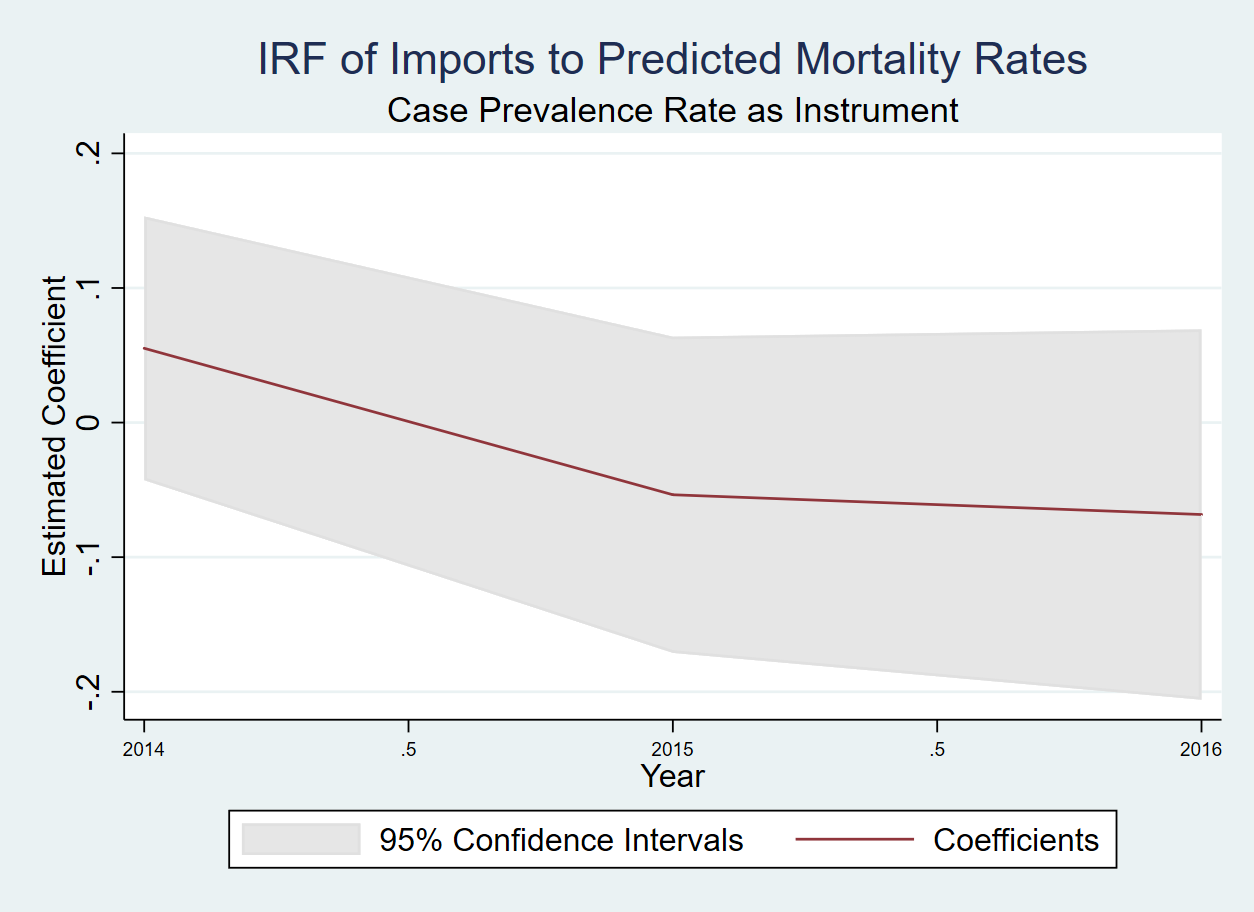
\includegraphics[width=\textwidth]{C:/Users/mariu/Documents/Master_Thesis/Master_thesis/Pics_graphs/IRF_second_imp_prev.png}\\
\end{minipage}\hfill% 
\caption{This figure shows the collection of local projections impulse response functions following \cite{jorda2005estimation} without including any control variables. The left half has the prevalence of Ebola cases as the measure for Ebola. On the right side, the measure for Ebola is the number of Ebola-related articles in the NYT. The maroon line marks the estimated coefficients while the shaded areas indicates the 95\% confidence intervals.}
\label{Second Stage IRF - no controls}
\end{figure}

The inclusion of control variables does not change the core message of the empirical estimation. Figure \ref{Second Stage IRF - controls} shows a similar trend for exports and imports to before with downward-corrected estiamtes for the second period. \\
Results do not really change for the trade balance, either. The right part of Figure \ref{IRF - Trade Balance} shows this. Most notably, the confidence intervals are way larger than they were before adding further doubt to the relevance of health.

\begin{figure}[!ht] 
\begin{minipage}[t]{0.5\linewidth}\vspace{0pt} 
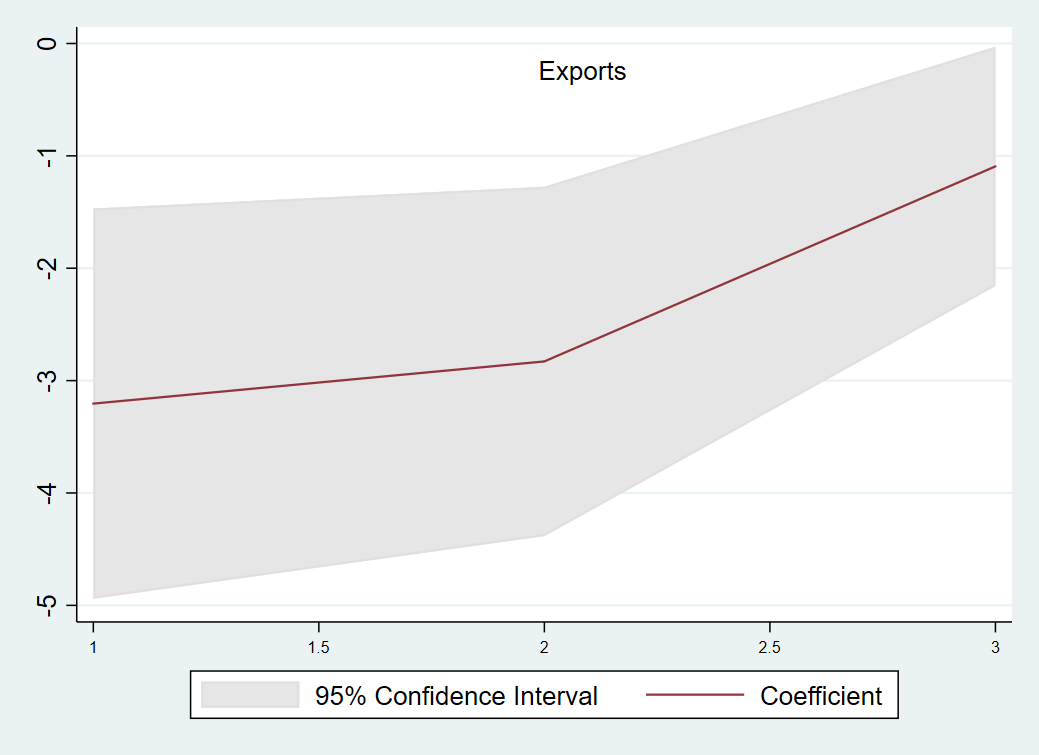
\includegraphics[width=\textwidth]{C:/Users/mariu/Documents/Master_Thesis/Master_thesis/Pics_graphs/IRF_second_control_exp.png}\\
\end{minipage}\hfill% 
\begin{minipage}[t]{0.5\linewidth}\vspace{0pt} 
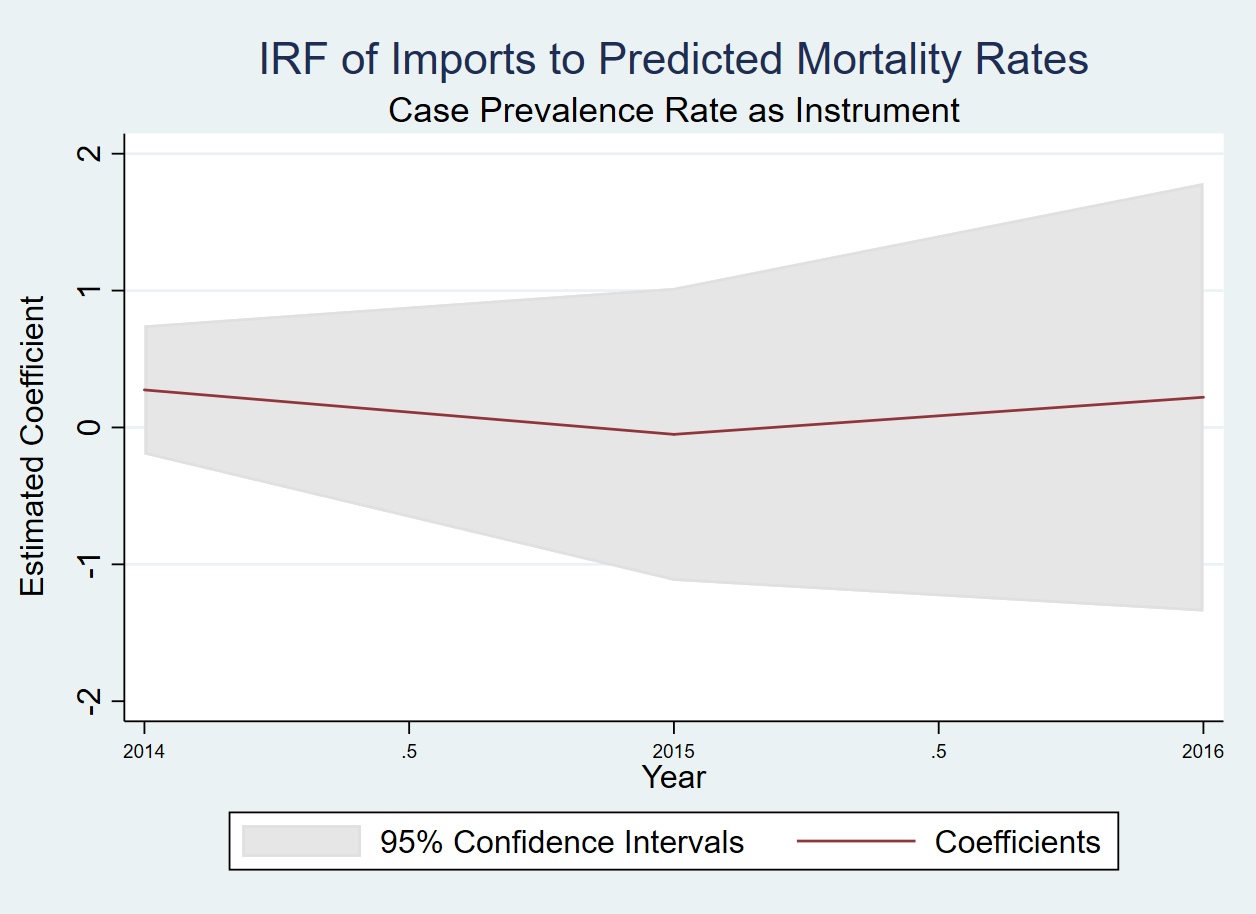
\includegraphics[width=\textwidth]{C:/Users/mariu/Documents/Master_Thesis/Master_thesis/Pics_graphs/IRF_second_control_imp.png}\\
\end{minipage}\hfill% 
\caption{This figure shows the collection of local projections impulse response functions following \cite{jorda2005estimation} without including any control variables. The left half has the prevalence of Ebola cases as the measure for Ebola. On the right side, the measure for Ebola is the number of Ebola-related articles in the NYT. The maroon line marks the estimated coefficients while the shaded areas indicates the 95\% confidence intervals.}
\label{Second Stage IRF - controls}
\end{figure}

\begin{figure}[!ht] 
\begin{minipage}[t]{0.5\linewidth}\vspace{0pt} 
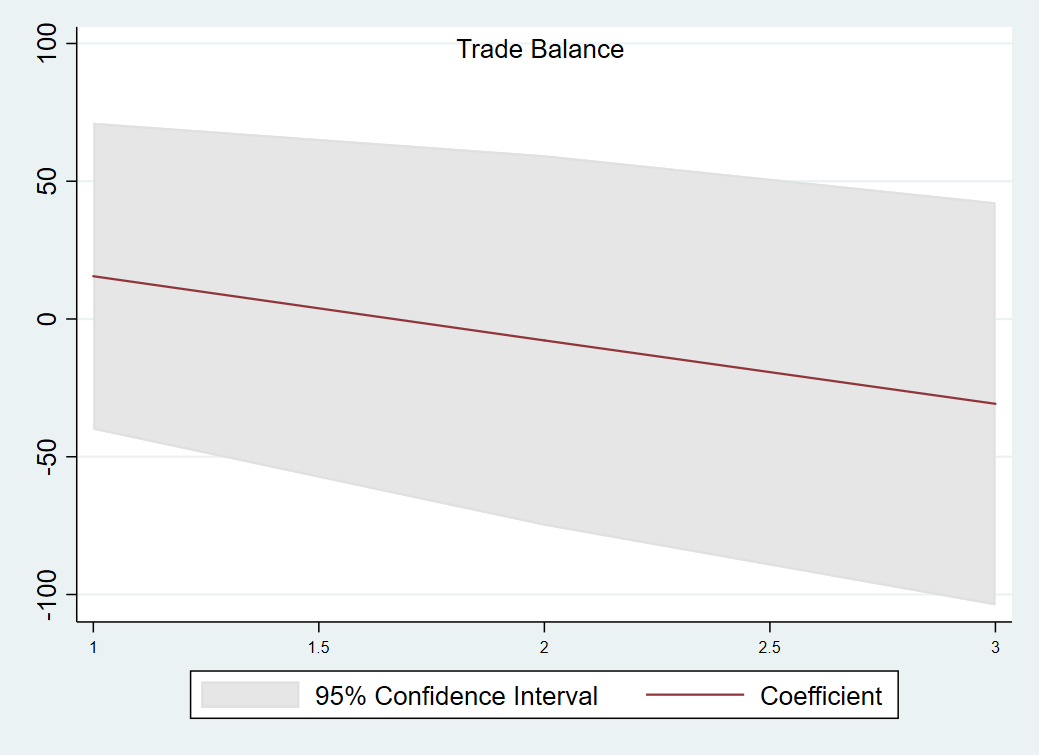
\includegraphics[width=\textwidth]{C:/Users/mariu/Documents/Master_Thesis/Master_thesis/Pics_graphs/IRF_second_tb_prev.png}\\
\end{minipage}\hfill% 
\begin{minipage}[t]{0.5\linewidth}\vspace{0pt} 
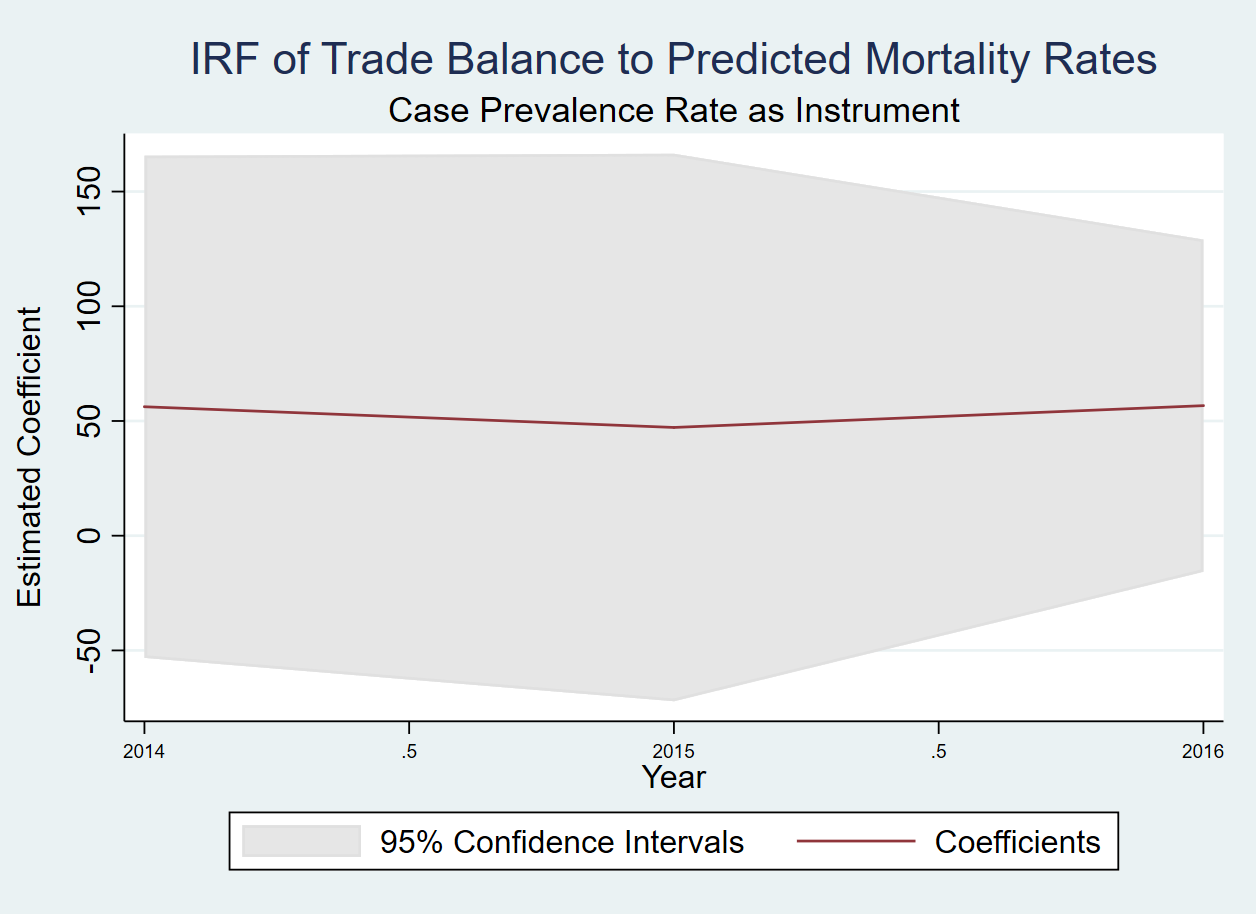
\includegraphics[width=\textwidth]{C:/Users/mariu/Documents/Master_Thesis/Master_thesis/Pics_graphs/IRF_second_control_tb.png}\\
\end{minipage}\hfill% 
\caption{This figure shows the collection of local projections impulse response functions following \cite{jorda2005estimation} without including any control variables. The left half has the prevalence of Ebola cases as the measure for Ebola. On the right side, the measure for Ebola is the number of Ebola-related articles in the NYT. The maroon line marks the estimated coefficients while the shaded areas indicates the 95\% confidence intervals.}
\label{IRF - Trade Balance}
\end{figure}

\section{Conclusion}


\pagebreak

\bibliography{job}
\bibliographystyle{ecta}

\pagebreak
\section{Appendix}


\subsection*{Figures}
\begin{figure}[!ht]
\begin{center}\caption{Baseline Simulation Extended \label{Baseline Simulation Extended}}
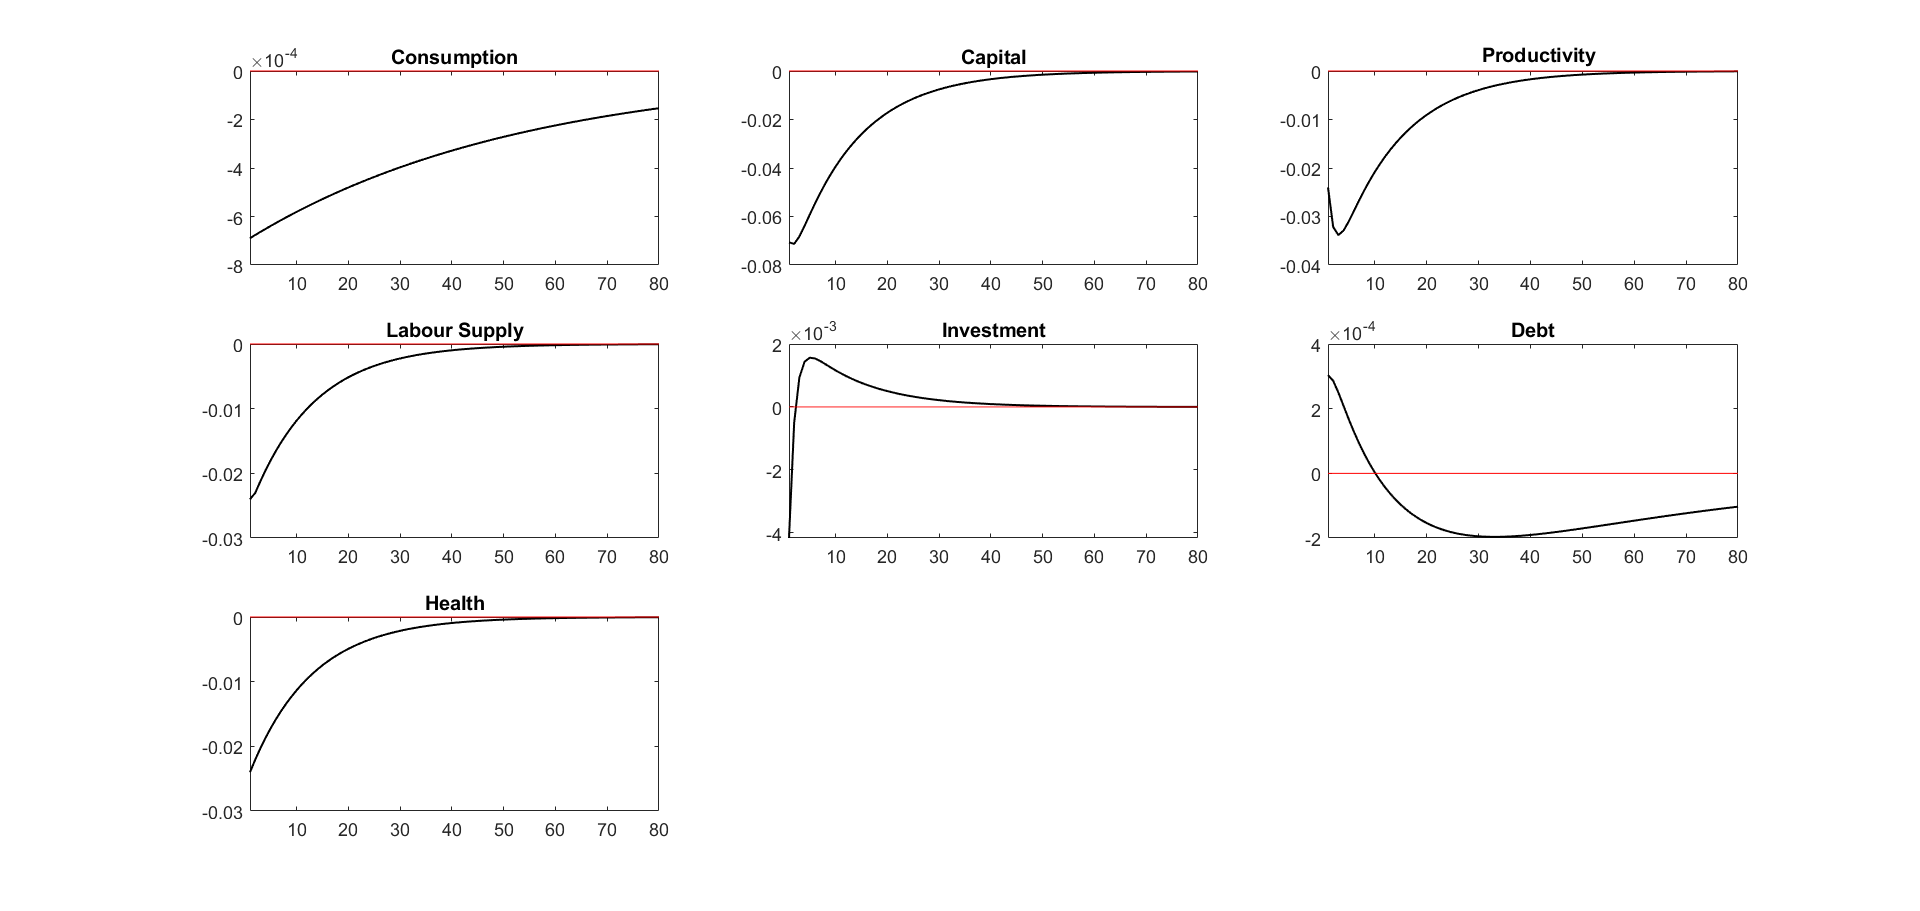
\includegraphics[width=1\textwidth]{C:/Users/mariu/Documents/Master_Thesis/Master_thesis/Pics_graphs/Simple_simulation_home_extended.png}\\
\end{center}
\end{figure}

\begin{figure}[!ht]
\begin{center}\caption{Baseline Simulation Foreign \label{Baseline Simulation Foreign}}
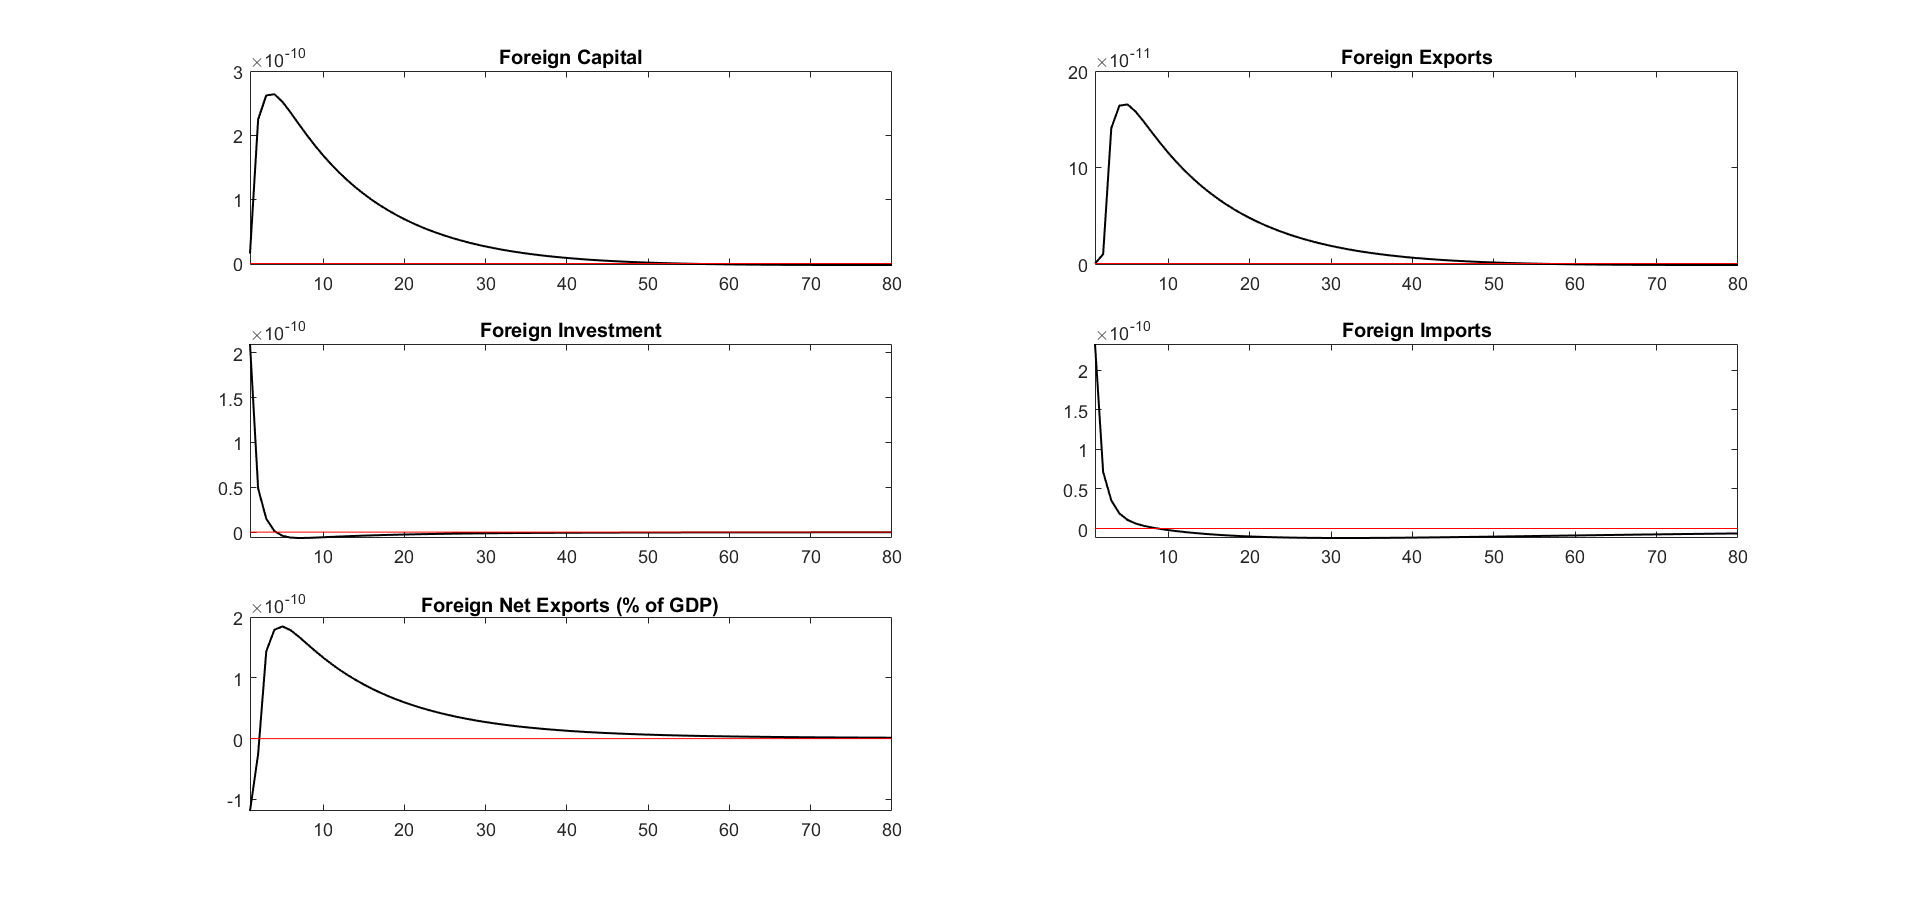
\includegraphics[width=1\textwidth]{C:/Users/mariu/Documents/Master_Thesis/Master_thesis/Pics_graphs/Simple_simulation_foreign_responses.png}\\
\end{center}
\end{figure}


\subsection*{Codes}

\newsavebox\myv
\begin{lrbox}{\myv}\begin{minipage}{\textwidth}
\begin{verbatim}
apikey <- '5801c0ee00824b7db6ca5a954495d112'

base_url <- "http://api.nytimes.com/svc/search/v2/articlesearch.json"
# install.packages("httr")
library(httr)

r <- GET(base_url, query=list(q="Ebola","api-key"=apikey))
r




nyt_count <- function(q, date1, date2){
  r <- GET(base_url, query=list(q=q,
                                "api-key"=apikey,
                                "begin_date"=date1,
                                "end_date"=date2))
  json <- content(r, "parsed")
  ## if there is no response
  while (r$status_code!=200){
    Sys.sleep(2) # wait a couple of seconds
    # try again:
    r <- GET(base_url, query=list(q=q,
                                  "api-key"=apikey,
                                  "begin_date"=date1,
                                  "end_date"=date2))
    json <- content(r, "parsed")
  }
  return(json$response$meta$hits)
}

nyt_dates_count <- function(q, init, end, by){
  # sequence of dates to loop over
  dates <- seq(from=init, to=end, by=by)
  dates <- format(dates, "%Y%m%d") # changing format to match NYT API format
  counts <- rep(NA, length(dates)-1)
  # loop over periods
  for (i in 1:(length(dates)-1)){ ## note the -1 here
    # information message to track progress
    message(dates[i])
    # retrieve count
    counts[i] <- nyt_count(q=q, date1=dates[i],
                           date2=dates[i+1])
  }
  # improving this as well so that it returns a data frame
  df <- data.frame(date = as.Date(dates[-length(dates)], format="%Y%m%d"), count = counts)
  return(df)
}

counts <- nyt_dates_count(q="Ebola Liberia", init = as.Date("2005/01/01"), end = as.Date("2018/10/30"), by="month")


plot(counts$date, counts$count, type="l", main="Mentions of 'Ebola in Liberia' in the NYT, by month",
     xlab="Month", ylab="Article count")

library(foreign)
write.dta(counts, "Articles_Ebola_Liberia.dta")
\end{verbatim}
\end{minipage}\end{lrbox}
\resizebox{0.75\textwidth}{!}{\usebox\myv}



\subsection*{Tables}

\begin{table}[htbp]\centering \caption{Estimated Second Order Moments \label{Estimated Second Order Moments}}
\begin{tabular}{l c c}\hline\hline
Variable & Estimated Variance & Variance in Data\\ \hline
Exports & 0.04 & 2.05 \\
Imports & 0.001 & 1.9 \\
Net Exports (\% of GDP) & 0.04 & 0.000 \\ \hline
\end{tabular}
\end{table}

\begin{center}
\begin{table}[htbp]\centering \caption{Summary Statistics\label{Appendix - Data}}
\resizebox{\textwidth}{!}{
\begin{tabular}{l c c c c c} \hline \hline
\multicolumn{1}{c} {\textbf{Variable}} & \textbf{Mean}
 & \textbf{Std. Dev.}& \textbf{Min.} &  \textbf{Max.} & \textbf{N}\\
\hline\hline
\multicolumn{6}{c} {Panel A - Health measures} \\ \hline
Adult mortality rate & 331.29 & 88.83 & 185 & 637 & 110296\\
Adult mortality (male) & 354.65 & 87.32 & 221 & 714 & 110296\\
Adult mortality (female) & 308.73 & 91.60 & 153 & 631 & 110296\\
Life expectancy & 56.50 & 5.39 & 39.8 & 68.7 & 107368\\
Life expectancy male & 55.24 & 5.18 & 38.5 & 66.7 & 107368\\
Life expectancy female & 57.79 & 5.65 & 40.7 & 70.7 & 107368\\
Infant mortality rate & 69.07 & 22.25 & 26.1 & 142 & 110296\\
Neonatal mortality rate & 33.55 & 8.31 & 14.9 & 57.2 & 110296\\
Under 5 mortality rate & 109.42 & 39.49 & 33.7 & 233.1 & 110296\\
Crude death rate & 11.7 & 3.33 & 5.732 & 23.99 & 110296\\
Anemia children & 67.11 & 11.16 & 36.2 & 89.90 & 110296\\
Anemia Women & 44.18 & 10.27 & 19 & 65.3 & 110296\\
\hline \hline
\multicolumn{6}{c}{Panel B - Output Statistics}\\ \hline
Imports (in Mil) & 40.73 & 238.02 & 0.00 & 15449.27 & 66922\\
Exports (in Mil.) & 51.81 & 583.82 & 0 & 33710.03 & 57794\\
Trade balance (in Mil.) & 5.87 & 446.14 & -6351.76 & 30252.98 & 79052\\
Current account (\% of GDP) & -7.34 & 10.67 & -86.09 & 21.75 & 87541\\
Real exchange rate & 103.46 & 37.41 & 53.71 & 516.28 & 40460\\
GDP p. c. & 925.49 & 710.13 & 193.87 & 3846.24 & 108441\\
\hline \hline
\multicolumn{6}{c}{Panel C - Control Variables}\\  \hline
Internet access & 4.87 & 6.52 & 0.01 & 41.21 & 108999\\
Percent migrants & 2.54 & 2.68 & 0.13 & 14.85 & 25806\\
Population density ($km^2$) & 79.26 & 90.60 & 2.63 & 483.08 & 109559\\
Living Rural (of Pop. & 64.36 & 13.66 & 28.91 & 91.75 & 109576\\
Living Urban (of Pop.) & 35.64 & 13.66 & 8.25 & 71.09 & 109576\\
Health expenditure (of GDP) & 5.54 & 2.22 & 1.44 & 19.73 & 98580\\
Net FDI (in million) & -569.45 & 1597.32 & -8235.47 & 13164.18 & 86502\\
Price Index & 93.79 & 39.51 & 2.91 & 1592.39 & 99330\\
Tariff rate & 13.66 & 3.78 & 0.78 & 25.17 & 80107\\
Education expenditure & 3.86 & 1.8 & 0.83 & 13.22 & 67861\\
Primary education & 38.70 & 21.18 & 5.17 & 88.02 & 7217\\
Savings & 10.851 & 16.25 & -141.97 & 64.93 & 100298\\
Fatalitites & 360.62 & 1100.26 & 0 & 11546 & 109835 \\
\hline \hline
\multicolumn{6}{c}{Panel D -Other Diseases}\\ \hline

Prevalence of HIV & 51.09 & 43.92 & 1 & 145 & 118716\\
Incidence Tuberculosis per 100,000 & 178.88 & 103.86 & 1 & 367 & 120940\\
Incidence of malaria per 1000 & 176.39 & 100.66 & 1 & 347 & 56231\\
Malaria cases reported & 154.13 & 85.15 & 1 & 301 & 46889\\
CVD, cancer, diabetes or CRD & 49.63 & 26.51 & 1 & 105 & 35795\\
Diabetes prevalence & 10.28 & 4.95 & 1 & 20 & 40\\

\hline
\end{tabular}
}
\end{table}
\end{center}


\begin{table}[htbp] \centering \caption{Event Study Estimates\label{Appendix - Event Study}}
\centering
\resizebox{0.7 \textwidth}{!}{
\begin{tabular}{lc} \hline
 & (1) \\
Variables & Event Study \\ \hline
\vspace{4pt} & \begin{footnotesize}\end{footnotesize} \\
new\_pre\_avg\_g10 & 24.38 \\
\vspace{4pt} & \begin{footnotesize}(33.34)\end{footnotesize} \\
new\_pre\_avg\_9 & 23.10 \\
\vspace{4pt} & \begin{footnotesize}(21.11)\end{footnotesize} \\
new\_pre\_avg\_8 & 20.78 \\
\vspace{4pt} & \begin{footnotesize}(20.39)\end{footnotesize} \\
new\_pre\_avg\_7 & 13.33 \\
\vspace{4pt} & \begin{footnotesize}(19.32)\end{footnotesize} \\
new\_pre\_avg\_6 & 12.37 \\
\vspace{4pt} & \begin{footnotesize}(16.47)\end{footnotesize} \\
new\_pre\_avg\_5 & 7.617 \\
\vspace{4pt} & \begin{footnotesize}(14.62)\end{footnotesize} \\
new\_pre\_avg\_4 & -3.642 \\
\vspace{4pt} & \begin{footnotesize}(14.13)\end{footnotesize} \\
new\_pre\_avg\_3 & -11.57 \\
\vspace{4pt} & \begin{footnotesize}(10.91)\end{footnotesize} \\
new\_pre\_avg\_2 & -11.54* \\
\vspace{4pt} & \begin{footnotesize}(6.158)\end{footnotesize} \\
new\_avg & 178.9*** \\
\vspace{4pt} & \begin{footnotesize}(17.81)\end{footnotesize} \\
new\_post\_avg\_1 & 57.45*** \\
\vspace{4pt} & \begin{footnotesize}(21.00)\end{footnotesize} \\
new\_post\_avg\_2 & 41.21** \\
\vspace{4pt} & \begin{footnotesize}(18.48)\end{footnotesize} \\
time & -0.0237*** \\
 & \begin{footnotesize}(0.00278)\end{footnotesize} \\
\vspace{4pt} & \begin{footnotesize}\end{footnotesize} \\
Observations & 124,106 \\
Number of id & 7,301 \\
 $R^2$ & 0.635 \\ \hline
\multicolumn{2}{c}{\begin{footnotesize} Clustered standard errors in parentheses\end{footnotesize}} \\
\multicolumn{2}{c}{\begin{footnotesize} *** p$<$0.01, ** p$<$0.05, * p$<$0.1\end{footnotesize}} \\
\multicolumn{2}{c}{\begin{footnotesize} The baseline year is set at $\tau - 1$, the year before the intervention. \end{footnotesize}} \\ 
\multicolumn{2}{c}{\begin{footnotesize} $trend$ represents a country-specific, linear trend.  \end{footnotesize}} \\
\end{tabular}
}
\end{table}


\begin{figure}[!ht]
\begin{center}\caption{Event Study Robustness \label{Event Study Robustness}}
\includegraphics[width=0.8\textwidth]{C:/Users/mariu/Documents/Master_Thesis/Master_thesis/Pics_graphs/Event_study_robustness.png}\\
\end{center}
\end{figure}


\begin{table}[htbp] \caption{IRF unstandardized results \label{Appendix - IRF unstandardized}}
\begin{tabular}{lcccc} \hline
 & (1) & (2) & (3) & (4)\\
Time & Case prevalence & Articles & Case prevalence & Articles\\ \hline
\vspace{4pt} & \begin{footnotesize}\end{footnotesize} & \begin{footnotesize}\end{footnotesize} & \begin{footnotesize}\end{footnotesize} \\
$\tau$ & 0.972*** & 0.0203***  & 1.15*** & 0.0147***\\
\vspace{4pt} & \begin{footnotesize}(0.317)\end{footnotesize} & \begin{footnotesize}(0.0039)\end{footnotesize} & \begin{footnotesize}(0.3013)\end{footnotesize} & \begin{footnotesize}(0.0049)\end{footnotesize}\\
$\tau + 1$ &  -0.123* & 0.0056** & -0.7025*  & 0.0037\\
 & \begin{footnotesize}(0.0657)\end{footnotesize} & \begin{footnotesize}(0.0025)\end{footnotesize} & \begin{footnotesize}(0.3975)\end{footnotesize} & \begin{footnotesize}(.0063)\end{footnotesize} \\
 $\tau + 2$ &  -0.951*** & -0.0142*** & -1.0209** & -0.0078\\
 & \begin{footnotesize}(0.0401)\end{footnotesize} & \begin{footnotesize}(.0038)\end{footnotesize} & \begin{footnotesize}(0.3909)\end{footnotesize} & \begin{footnotesize}(.0081)\end{footnotesize}\\
\vspace{4pt} & \begin{footnotesize}\end{footnotesize} & \begin{footnotesize}\end{footnotesize} & \begin{footnotesize}\end{footnotesize} & \begin{footnotesize}\end{footnotesize}\\
Control Var. & No & No & Yes & Yes \\ \hline
\multicolumn{4}{c}{\begin{footnotesize} Robust standard errors in parentheses\end{footnotesize}} \\
\multicolumn{4}{c}{\begin{footnotesize} *** p$<$0.01, ** p$<$0.05, * p$<$0.1\end{footnotesize}} \\
\end{tabular}
\end{table}


\begin{table}[htbp]\centering \caption{Balance of clusters \label{Balance of clusters}}
\begin{tabular}{l c c}\hline\hline
\textbf{Cluster Number} & \textbf{N}
 & \textbf{Percent} \\ \hline
N\_1 & 5287 & 4.15 \\
N\_2 & 3468 & 2.72  \\
N\_3 & 3264 & 2.56 \\
N\_4 & 3026 & 2.38 \\
N\_5 & 3485 & 2.74 \\
N\_6 & 5899 & 4.63 \\
N\_7 & 3128 & 2.46 \\
N\_8 & 2550 & 2   \\
N\_9 & 3315 & 2.6  \\
N\_10 & 3502 & 2.75\\
N\_11 & 2431 & 1.91\\
N\_12 & 2839 & 2.23\\
N\_13 & 3213 & 2.52\\
N\_14 & 3366 & 2.64\\
N\_15 & 3553 & 2.79\\
N\_16 & 3417 & 2.68\\
N\_17 & 2550 & 2  \\
N\_18 & 3485 & 2.74 \\
N\_19 & 2295 & 1.8  \\
N\_20 & 1530 & 1.2  \\
N\_21 & 3417 & 2.68 \\
N\_22 & 3502 & 2.75 \\
N\_23 & 3519 & 2.76 \\
N\_24 & 3502 & 2.75 \\
N\_25 & 3502 & 2.75 \\
N\_26 & 3400 & 2.67 \\
N\_27 & 3468 & 2.72 \\
N\_28 & 3536 & 2.78 \\
N\_29 & 3213 & 2.52 \\
N\_30 & 3349 & 2.63 \\
N\_31 & 2856 & 2.24 \\
N\_32 & 1241 & 0.97 \\
N\_34 & 3026 & 2.38\\
N\_35 & 3502 & 2.75\\
N\_36 & 3400 & 2.67\\
N\_37 & 3247 & 2.55\\
N\_38 & 3417 & 2.68\\
N\_39 & 3417 & 2.68 \\ \hline
\multicolumn{3}{c}{\begin{footnotesize} Cluster 33 has no observation \end{footnotesize}} \\
\multicolumn{3}{c}{\begin{footnotesize}  and is therefore not listed.
\end{footnotesize}}
\end{tabular}
\end{table}

\begin{figure}[!ht] 
\begin{minipage}[t]{0.5\linewidth}\vspace{0pt} 
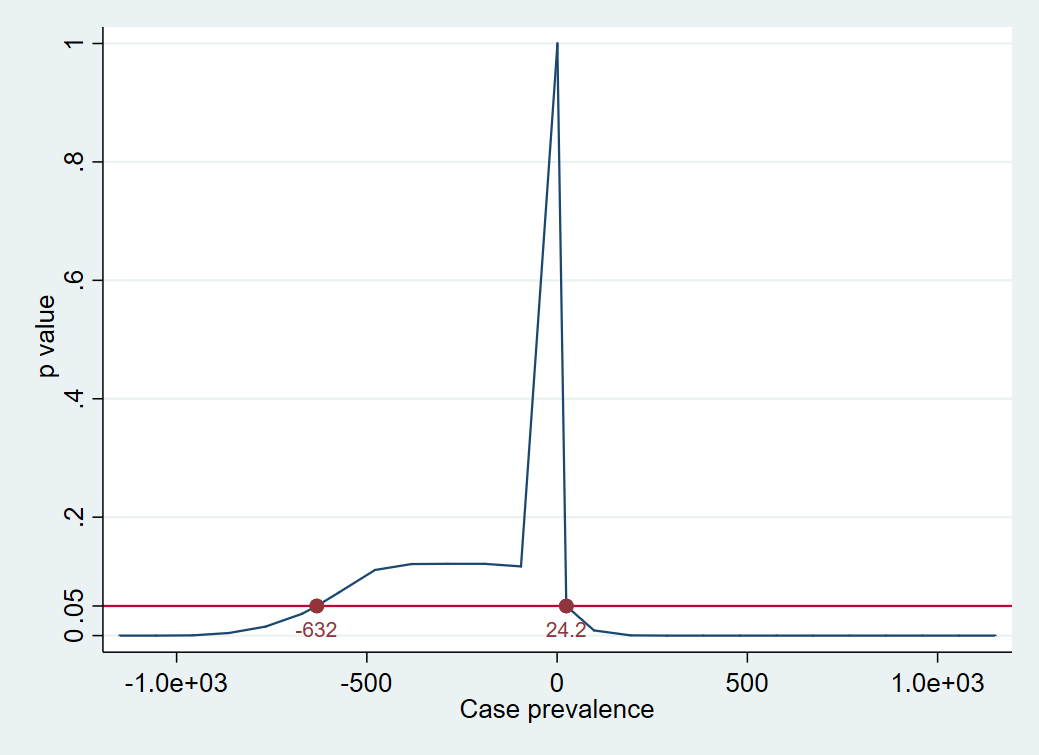
\includegraphics[width=\textwidth]{C:/Users/mariu/Documents/Master_Thesis/Master_thesis/Pics_graphs/Prev_no_controls_restricted_wild_bootstrap.png}\\
\vspace{2ex}
\end{minipage}\hfill% 
\begin{minipage}[t]{0.5\linewidth}\vspace{0pt} 
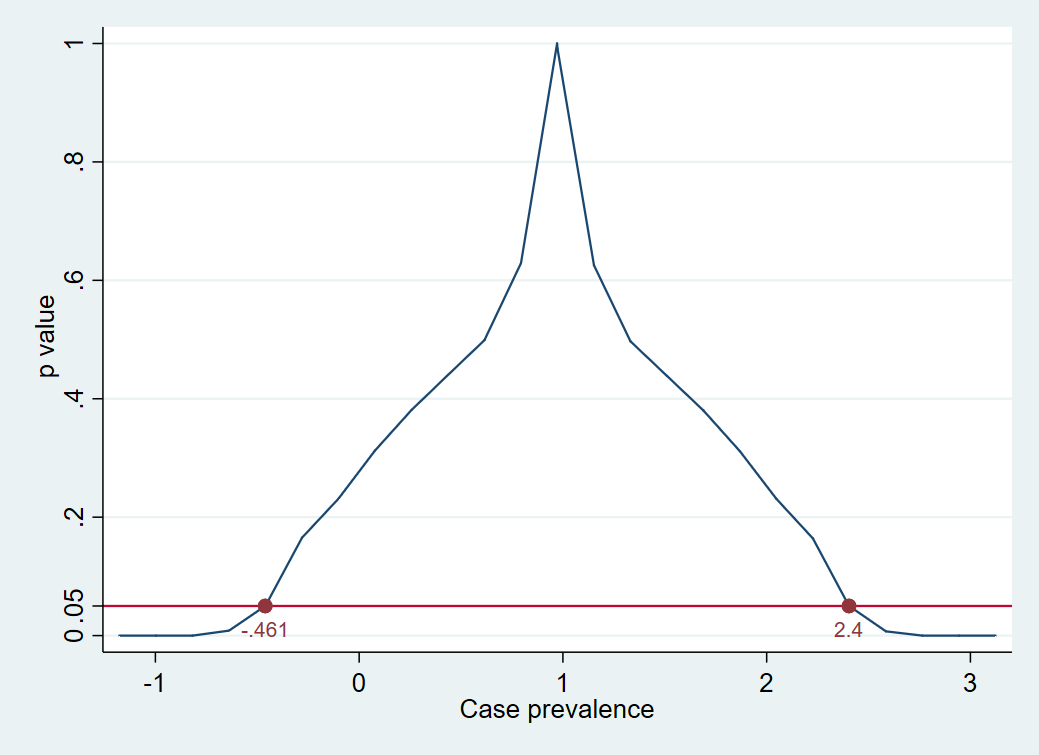
\includegraphics[width=\textwidth]{C:/Users/mariu/Documents/Master_Thesis/Master_thesis/Pics_graphs/Prev_no_controls_unresticted_wild_bootstrap.png}\\
\vspace{2ex}
\end{minipage}\hfill% 
\begin{minipage}[t]{0.5\linewidth}\vspace{0pt} 
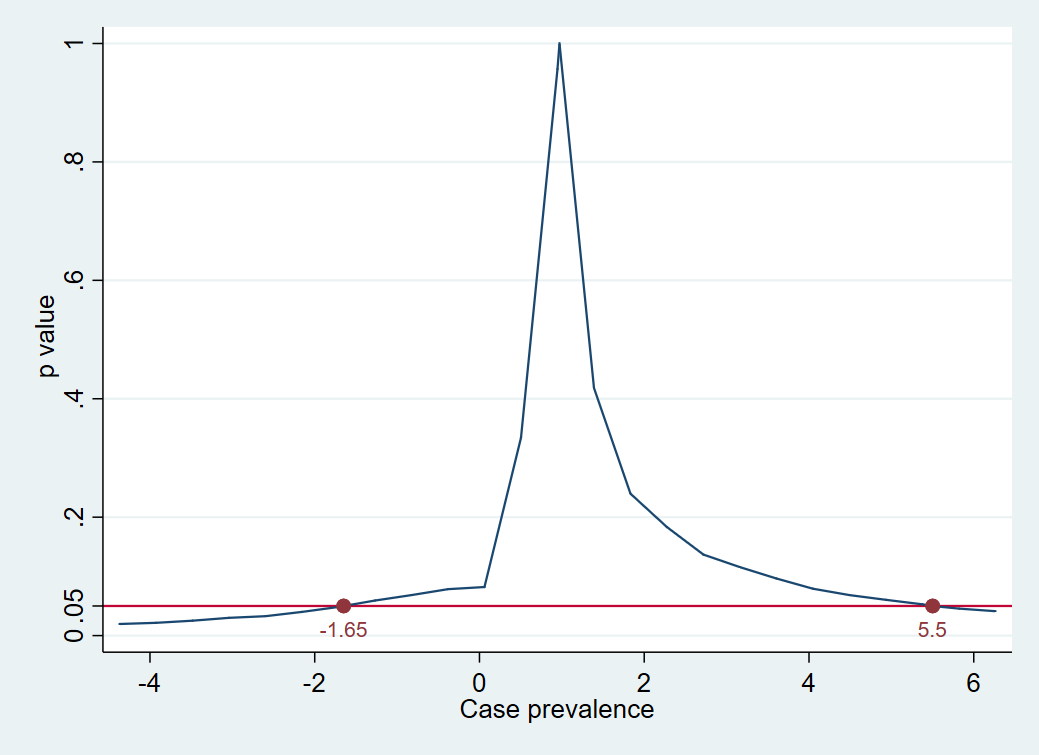
\includegraphics[width=\textwidth]{C:/Users/mariu/Documents/Master_Thesis/Master_thesis/Pics_graphs/Prev_no_controls_restricted_subclusters.png}\\
\vspace{2ex}
\end{minipage}\hfill% 
\begin{minipage}[t]{0.5\linewidth}\vspace{0pt} 
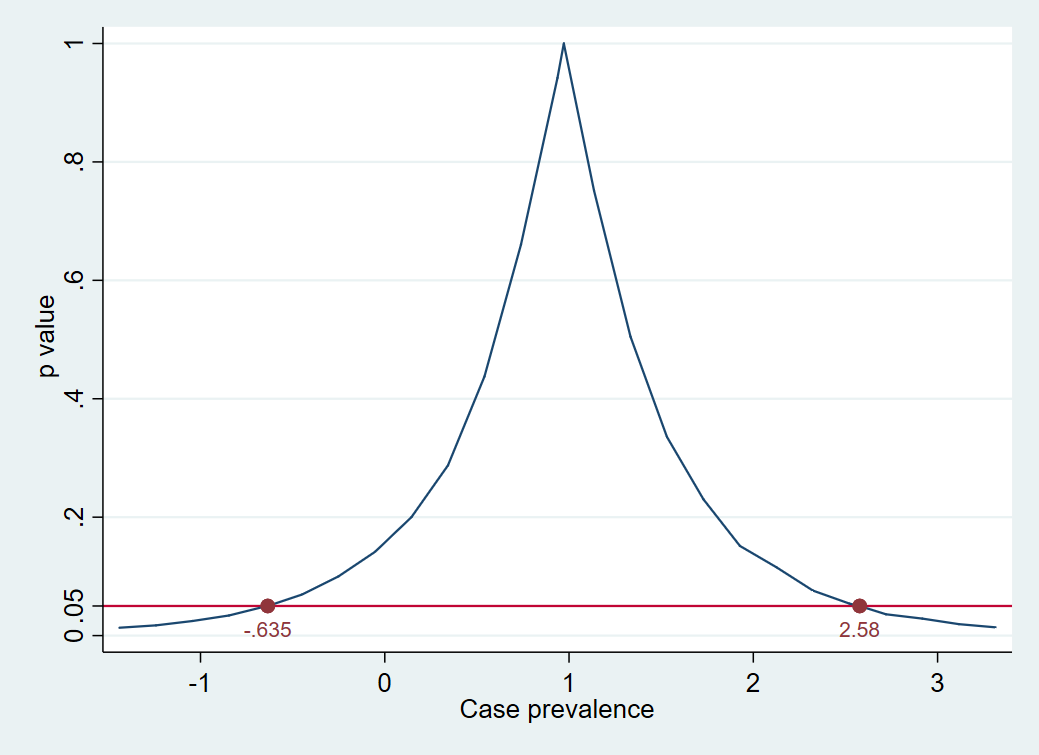
\includegraphics[width=\textwidth]{C:/Users/mariu/Documents/Master_Thesis/Master_thesis/Pics_graphs/Prev_no_controls_unrestricted_subclusters.png}\\
\vspace{2ex}
\end{minipage}\hfill% 
\caption{Shows the estimated confidence intervals. The results follow the baseline estimations in section ?? and include the case prevalence as the relevant measure.
The upper row shows bootstrap clustering at the country level, the lower at the country-pair level. The left side follows the procedure pioneered by \cite{cameron2008bootstrap}. The right column reports the additive procedure as in \cite{mackinnon2018wild}.} 
\label{Wild cluster bootstrap I}
\end{figure}

\begin{figure}[!ht] 
\begin{minipage}[t]{0.5\linewidth}\vspace{0pt} 
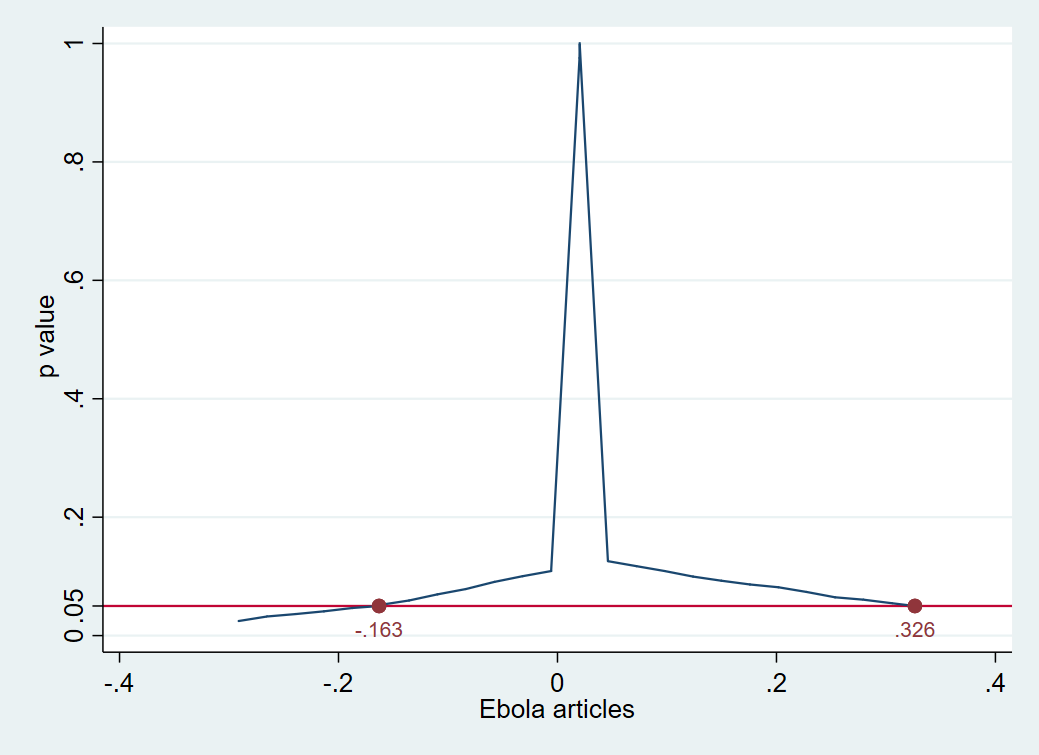
\includegraphics[width=\textwidth]{C:/Users/mariu/Documents/Master_Thesis/Master_thesis/Pics_graphs/Articles_restricted_country.png}\\
\vspace{2ex}
\end{minipage}\hfill% 
\begin{minipage}[t]{0.5\linewidth}\vspace{0pt} 
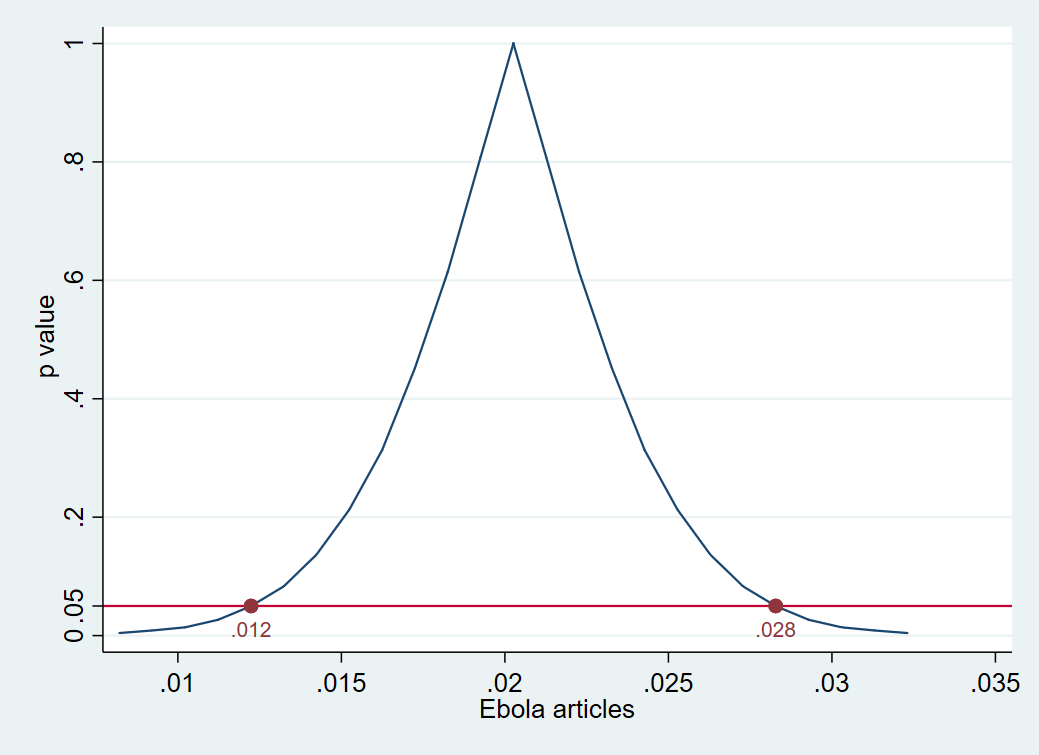
\includegraphics[width=\textwidth]{C:/Users/mariu/Documents/Master_Thesis/Master_thesis/Pics_graphs/Articles_unrestricted_country.png}\\
\vspace{2ex}
\end{minipage}\hfill% 
\begin{minipage}[t]{0.5\linewidth}\vspace{0pt} 
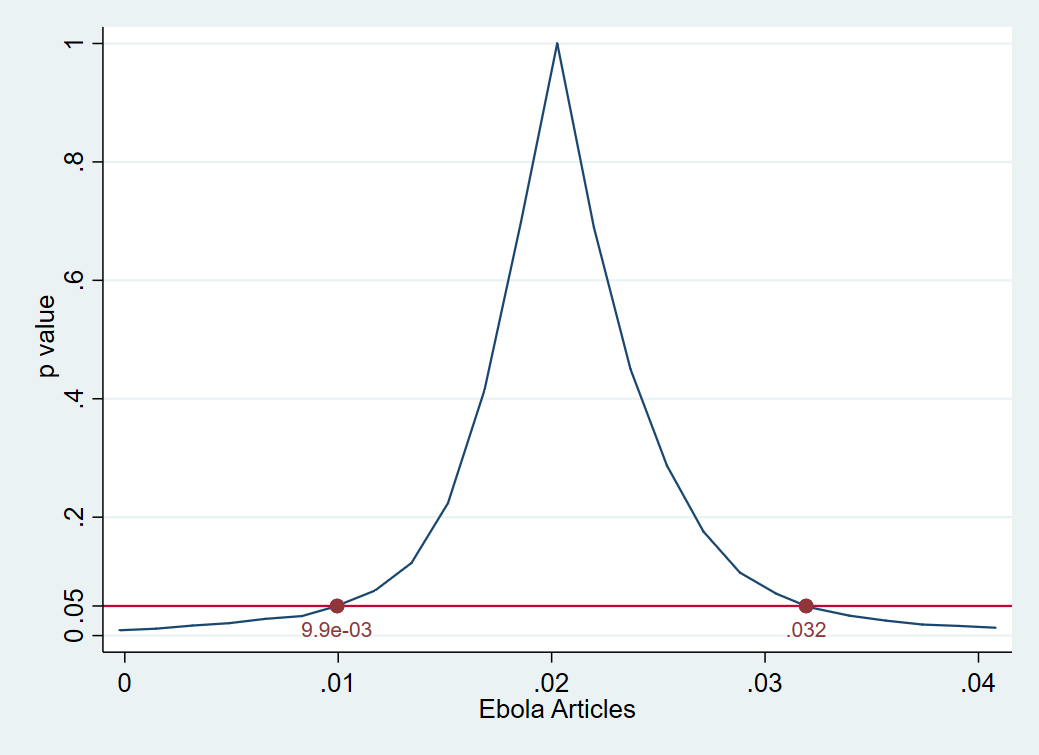
\includegraphics[width=\textwidth]{C:/Users/mariu/Documents/Master_Thesis/Master_thesis/Pics_graphs/Articles_restricted_subcluster.png}\\
\vspace{2ex}
\end{minipage}\hfill% 
\begin{minipage}[t]{0.5\linewidth}\vspace{0pt} 
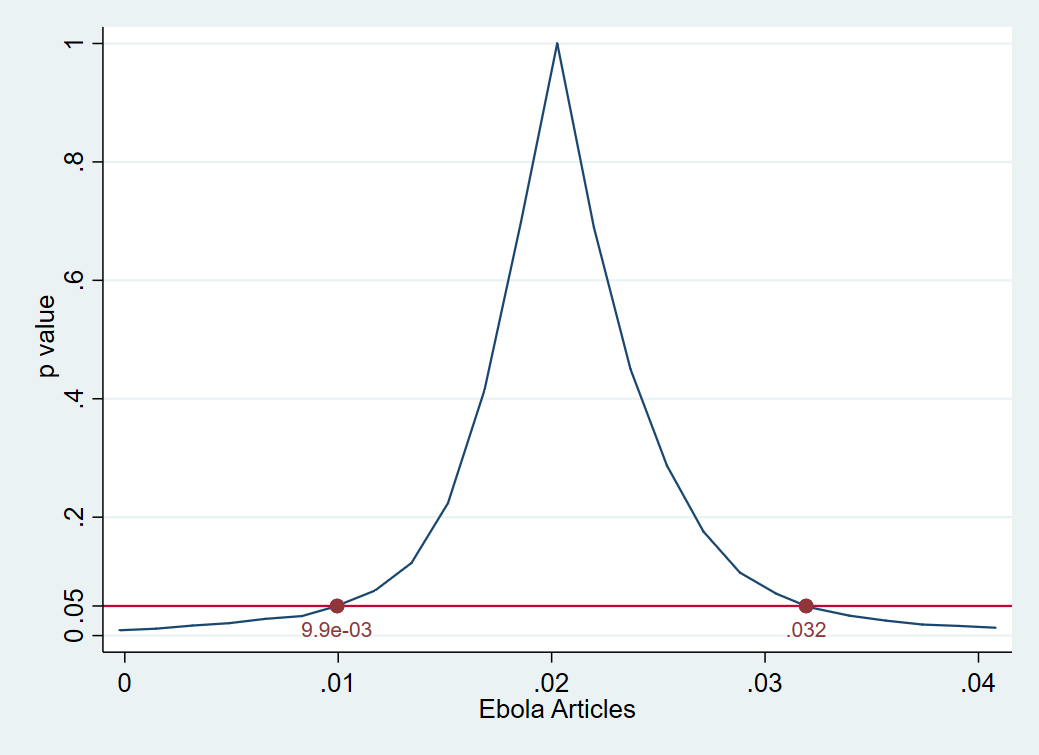
\includegraphics[width=\textwidth]{C:/Users/mariu/Documents/Master_Thesis/Master_thesis/Pics_graphs/Articles_restricted_subcluster.png}\\
\vspace{2ex}
\end{minipage}\hfill% 
\caption{Shows the estimated confidence intervals. The results follow the baseline estimations in section ?? and include the Ebola articles as the relevant measure.
The upper row shows bootstrap clustering at the country level, the lower at the country-pair level. The left side follows the procedure pioneered by \cite{cameron2008bootstrap}. The right column reports the additive procedure as in \cite{mackinnon2018wild}.} 
\label{Wild cluster bootstrap I}
\end{figure}

\end{document}